
%----------------+
%  Ph.D. Thesis  |
%----------------+

%--------------------------+
%  \tiny          5pt      |
%  \scriptsize    7pt      |
%  \footnotesize  8pt      |
%  \small         9pt      |
%  \normalsize    10pt     |
%  \large         12pt     |
%  \Large         14.4pt   |
%  \LARGE         17.28pt  |
%  \huge          20.74pt  |
%  \Huge          24.88pt  |
%--------------------------+

%	(j / js)article, report, book, etc.
\documentclass[11pt, twoside, titlepage]{article}

%	Driver that generates PDF from DVI, Important to insert images
\usepackage[dvipdfmx]{graphicx}

%	Link
\usepackage[dvipdfmx]{hyperref}

%	Important to change the style of each page
\usepackage{fancyhdr}

%	Space
\usepackage[top=25truemm, bottom=20truemm, left=25truemm, right=25truemm]{geometry}

%	Size of section & subsection
\usepackage{titlesec}
\titleformat*{\section}{\huge\bfseries}
\titleformat*{\subsection}{\LARGE\bfseries}
\titleformat*{\subsubsection}{\Large\bfseries}

%	Having to do with the position of image
\usepackage{float}

%	Amssymb & Amsmath & Amsfonts
\usepackage{amssymb, amsmath, amsfonts}

%	Bold italic
\usepackage{bm}

%	Braket
\usepackage{braket}

%	Caption
\usepackage{caption}
\captionsetup[figure]{font=small}
\captionsetup[table]{font=small}

%	Comment
\usepackage{comment}

%	Cite
\usepackage{cite}

%	Color
\usepackage{color}

%	Here
\usepackage{here}

%	Listings
\usepackage{listings}

%	Multirow
\usepackage{multirow}

\lstset{
language={C++}, 
basicstyle      = {\tt\normalsize},
identifierstyle = {\tt\normalsize},
commentstyle    = {\tt\normalsize \color[rgb]{0,0.5,0}},
keywordstyle    = {\tt\normalsize \color[rgb]{0,0,0}},
ndkeywordstyle  = {\tt\normalsize},
stringstyle     = {\tt\normalsize},
frame           = {tblr},
breaklines      = true,
breakindent     = 45.8pt, % 11pt
%breakindent    = 50.6pt, % 12pt
captionpos      = b
columns         = [l]{fullflexible},
morecomment     = [l]{//},
numbers         = none,
numbersep       = 1zw,
numberstyle     = {\scriptsize},
stepnumber      = 1,
}

%	Times new roman
\usepackage{times}

%	URL
\usepackage{url}
\urlstyle{rm}

%	Physics
%	\usepackage{physics}

%	Character corruption
\usepackage{pxjahyper}
\hypersetup{colorlinks=true, linkcolor=black, citecolor=blue}

%	Equation, figure and table number
\makeatletter
\@addtoreset{equation}{section}
\@addtoreset{figure}{section}
\@addtoreset{table}{section}
\def\theequation{\thesection.\arabic{equation}}
\def\thefigure{\thesection.\arabic{figure}}
\def\thetable{\thesection.\arabic{table}}
\makeatother

%	Important formulas
\newcommand{\bd}{{\rm n} \to {\rm p}+{\rm e}^{-}+\bar{\nu}_{\rm e}}
\newcommand{\ibd}{\bar{\nu}_{\rm e}\,+\,{\rm p} \to {\rm e}^{+}\,+\,{\rm n}}
\newcommand{\hs}{\hspace{6mm}}
\newcommand{\vs}{\vspace{3mm}}

%	Space between the lines
\renewcommand{\baselinestretch}{1.1}

%	Set of notes
\renewcommand\thefootnote{\arabic{footnote}}

%	Header and footer
\pagestyle{fancy}
\newcommand{\Headerfooter}[1]{
\lhead[{\bf \thepage}]{}
\rhead[\thesection. #1]{{\bf \thepage}}
\cfoot[]{}
}
\newcommand{\Noheaderfooter}{
\lhead[{\bf \thepage}]{}
\rhead[]{{\bf \thepage}}
\cfoot[]{}
}

%	Title page
\title{
\fontsize{17.28pt}{34.56pt}
\textbf{Measurement of the neutrino-oxygen}\\
\textbf{neutral-current quasielastic cross section}\\
\textbf{and study of nucleon-nucleus interaction model}\\
\textbf{using atmospheric neutrino data in the SK-Gd experiment}
\vspace{10mm}
}
\author{
{\LARGE March 15, 2024}                \vspace{3mm}\\
{\LARGE Seiya Sakai}                   \vspace{20mm}\\
{\LARGE Graduate School of}            \vspace{3mm}\\
{\LARGE Natural Science and Technology}\vspace{3mm}\\
{\LARGE (Doctor's Course)}             \vspace{3mm}\\
{\LARGE OKAYAMA UNIVERSITY}
}
\date{}

%	Title page
%\title{\fontsize{20pt}{40pt}\textbf{Measurement of the neutrino-oxygen}\\\textbf{neutral-current quasielastic cross section using}\\\textbf{atmospheric neutrinos in the SK-Gd experiment}}
%\author{{\Large Graduate School of Natural Science and Technology}\vspace{2mm}\\{\Large Okayama University}\vspace{10mm}\\ \fontsize{20pt}{40pt}\selectfont Seiya Sakai}
%\date{\vspace{3mm}{\Large March 1, 2024}}

%------------+
%  Document  |
%------------+

\begin{document}
\parindent=0pt

%	Title
\maketitle

%	Abstract

%
%	Abstract
%

\begin{center}
	{\LARGE\bfseries \textcolor{white}{White}}
\end{center}
\thispagestyle{empty}
\clearpage
\newpage


%
%	Abstract
%

\begin{center}
	{\LARGE\bfseries ABSTRACT}
\end{center}
\vs\hs Neutrino is neutrino.\\
Do you know neutrino?
\thispagestyle{empty}
\clearpage


%	Acknowledgments

%
%	Acknowledgments
%

\thispagestyle{empty}

\begin{center}
	{\LARGE\bfseries ACKNOWLEDGMENTS}
\end{center}
\vs\hs Thank you so much!
\thispagestyle{empty}


%	Table of contents & List of figures & List of tables
\pagenumbering{roman}
\setcounter{tocdepth}{3}
\Noheaderfooter
\tableofcontents
\newpage
\listoffigures
\newpage
\listoftables
\cleardoublepage

%	Main
\pagenumbering{arabic}

%
%	Section 1
%

\section{Introduction}\label{Section_Introd}
\Headerfooter{Introduction}

\subsection{Neutrino}
\vs\hs Neutrinos, which are Fermions with spin of 1$/$2, are classified as leptons that do not participate in the strong interaction in the Standard Model (SM) of the particle physics.
Moreover, neutrinos do not have charge, and the neutrino mass is so tiny that the gravitational interaction can be ignored.
Therefore, neutrinos interact with other particles only via the weak interaction, and are difficult to observe.
The name "neutrino" was named by E. Fermi in 1933~\cite{HistoryOfNeutrino}.
The name comes from the "neutral" that means the zero charge, and "ino" that means small in Italian.
Currently, we know that there are three flavors of neutrinos: electron neutrino, muon neutrino, and tau neutrino.\\
\hs The existence of neutrinos was suggested by W. Pauli in 1930~\cite{HistoryOfNeutrino}.
Once, the energy spectrum of the electron emitted by the beta decay was expected to be the line spectrum.
However, in 1914, J. Chadwick found that the energy spectrum was not the line spectrum but the continuous spectrum~\cite{1914Chadwick}.
To explain the continuous spectrum of the electron reported by Chadwick, Pauli claimed that an unknown particle with spin of 1$/$2 and zero charge is emitted in the beta decay in addition to the electron.
In 1956, more than 20 years after Pauli proposed the existence of neutrinos, (electron anti)neutrinos produced in nuclear reactors were discovered by F. Reines and C. Cowan~\cite{1956Reines}.
In 1962, muon neutrinos were discovered in the accelerator experiment by L. Lederman, M. Schwartz, and J. Steinberger~\cite{1962Danby}.
In 2001, tau neutrinos were discovered in the DONUT (Direct Observation of NU Tau) experiment~\cite{2001Kodama}.

\subsection{Neutrino oscillation}
\vs\hs In the SM, the neutrino mass is zero~\cite{2022Workman}.
However, in 1998, the evidence for the neutrino oscillation was discovered in the Super-Kamiokande and it was proved that the neutrino mass is not zero~\cite{1998Fukuda}.
Neutrino oscillation is a phenomenon that the flavor of neutrino changes while the neutrino passes through a space.\\
\hs Here the neutrino oscillation in vacuum is considered.
The flavor eigenstate $\ket{\nu_{\alpha}}$ is represented by the superposition of the mass eigenstate $\ket{\nu_{i}}$,
\begin{eqnarray}
	\ket{\nu_{\alpha}}=\sum_{i=1}^{n} U_{\alpha i}^{*}\ket{\nu_{i}},
\end{eqnarray}
where $n$ ($=3$) is the number of neutrino species and $U$ is a 3$\,\times\,$3 unitary matrix, called the Pontecorvo-Maki-Nakagawa-Sakata (PMNS) mixing matrix.
This matrix consists of four independent parameters (three mixing angles, $\theta_{12}$, $\theta_{23}$, and $\theta_{13}$, and one phase angle $\delta_{{\rm CP}}$),
\begin{eqnarray}
	U&=&\left(
	\begin{array}{ccc}
		1&0&0\\
		0&c_{23}&s_{23}\\
		0&-s_{23}&c_{23}
	\end{array}
	\right)
	\left(
	\begin{array}{ccc}
		c_{13}&0&s_{13}e^{-i\delta_{{\rm CP}}}\\
		0&1&0\\
		-s_{13}e^{i\delta_{{\rm CP}}}&0&c_{13}
	\end{array}
	\right)
	\left(
	\begin{array}{ccc}
		c_{12}&s_{12}&0\\
		-s_{12}&c_{12}&0\\
		0&0&1
	\end{array}
	\right) \nonumber \\
	&=&\left(
	\begin{array}{ccc}
		c_{12}c_{13}&s_{12}c_{13}&s_{13}e^{-i\delta_{{\rm CP}}}\\
		-s_{12}c_{23}-c_{12}s_{23}s_{13}e^{i\delta_{{\rm CP}}}&c_{12}c_{23}-s_{12}s_{23}s_{13}e^{i\delta_{{\rm CP}}}&s_{23}c_{13}\\
		s_{12}s_{23}-c_{12}c_{23}s_{13}e^{i\delta_{{\rm CP}}}&-c_{12}s_{23}-s_{12}c_{23}s_{13}e^{i\delta_{{\rm CP}}}&c_{23}c_{13}
	\end{array}
	\right),
\end{eqnarray}
where $c_{ij}\equiv\cos\theta_{ij}$ and $s_{ij}\equiv\sin\theta_{ij}$.
After traveling a distance $L$ ($\simeq ct$ for relativistic neutrinos), the flavor eigenstate evolves as
\begin{eqnarray}
	\ket{\nu_{\alpha}(t)}=\sum_{i=1}^{n} U_{\alpha i}^{*}\ket{\nu_{i}(t)},
\end{eqnarray}
where $\ket{\nu_{i}(t)}=e^{-iE_{i}t}\ket{\nu_{i}(0)}$ ($E_{i}$ is the energy of the neutrino mass eigenstate $\nu_{i}$).
At that time, the probability of being observed as the flavor eigenstate $\ket{\nu_{\beta}}$ is
\begin{eqnarray}\label{Introd_Eq_Prob}
	P_{\alpha\beta}=|\braket{\nu_{\beta}|\nu_{\alpha}(t)}|^{2}=\Bigg|\sum_{i=1}^{n}\sum_{j=1}^{n} U_{\alpha i}^{*}U_{\beta j}\braket{\nu_{j}|\nu_{i}(t)}\Bigg|^{2}.
\end{eqnarray}
Here, neutrinos are relativistic, thus $p_{i} \simeq p_{j} \equiv p \simeq E$. Therefore, $E_{i}$ can be approximated as
\begin{eqnarray}\label{Introd_Eq_E}
	E_{i} = \sqrt{p_{i}^{2}+m_{i}^{2}} = p_{i}\sqrt{1+{m_{i}^{2} \over p_{i}^{2}}} \simeq p_{i}\Bigg(1+{m_{i}^{2} \over 2p_{i}^{2}}\Bigg) \simeq E+{m_{i}^{2} \over 2E}.
\end{eqnarray}
Using Equation (\ref{Introd_Eq_E}) and the orthogonality of the mass eigenstates, $\braket{\nu_{j}|\nu_{i}}=\delta_{ij}$, Equation (\ref{Introd_Eq_Prob}) can be expressed as
\begin{eqnarray}
	P_{\alpha\beta}=\delta_{\alpha\beta}-4\sum_{i<j}^{n} {\rm Re}[U_{\alpha i}U_{\beta i}^{*}U_{\alpha j}^{*}U_{\beta j}]\sin^{2}X_{ij}+2\sum_{i<j}^{n} {\rm Im}[U_{\alpha i}U_{\beta i}^{*}U_{\alpha j}^{*}U_{\beta j}]\sin 2X_{ij},
\end{eqnarray}
where
\begin{eqnarray}
	X_{ij} = {(m_{i}^{2}-m_{j}^{2})L \over 4E} \equiv {\Delta m_{ij}^{2}L \over 4E} = 1.267{\Delta m_{ij}^{2} \over {\rm eV}^{2}}{L/E \over {\rm m}/{\rm MeV}}.
\end{eqnarray}
The neutrino oscillation between two neutrino species in vacuum is described in Appendix~\ref{AppA}.
Moreover, the neutrino oscillation in matter is described in Ref.~\cite{1989Kuo}.\\
\hs From the above calculation, it can be seen that the neutrino oscillation can be described by six parameters ($\theta_{12}$, $\theta_{23}$, $\theta_{13}$, $\Delta m_{21}^{2}$, $\Delta m_{32}^{2}$, and $\delta_{{\rm CP}}$).
These parameters can be measured by observing the oscillation phenomena of solar neutrinos, atmospheric neutrinos, reactor neutrinos, and accelerator neutrinos.
Table~\ref{Introd_Tab:Neu} shows the three-neutrino mixing parameters and $\delta_{{\rm CP}}$.
Currently, the values of $m_{1}$, $m_{2}$, and $m_{3}$ and the magnitude relationship between $m_{2}$ and $m_{3}$ are not yet known.
There are two possibilities of the neutrino mass ordering: Normal Ordering (NO, $m_{1}<m_{2}<m_{3}$) or Inverted Ordering (IO, $m_{3}<m_{1}<m_{2}$).

\begin{table}[h]
	\caption[Three-neutrino mixing parameters and $\delta_{{\rm CP}}$]{\label{Introd_Tab:Neu} Three-neutrino mixing parameters and $\delta_{{\rm CP}}$~\cite{PDG}. Here, $\theta_{ij}\in[0,\pi/2]$ and $\delta_{{\rm CP}}\in[0,2\pi]$.}
	\centering
	\vs
	\begin{tabular}{ll}
		\hline\hline
		$\sin^{2}\theta_{12}$&$0.307 \pm 0.013$\\
		$\sin^{2}\theta_{23}$ (NO)&$0.547\,^{+0.018}_{-0.024}$\\
		$\sin^{2}\theta_{23}$ (IO)&$0.534\,^{+0.021}_{-0.024}$\\
		$\sin^{2}\theta_{13}$&$(2.20 \pm 0.07) \times 10^{-2}$\\
		$\Delta m_{21}^{2}$&$(7.53 \pm 0.18) \times 10^{-5}\,{\rm eV}^{2}$\\
		$\Delta m_{32}^{2}$ (NO)&$(2.437 \pm 0.033) \times 10^{-3}\,{\rm eV}^{2}$\\
		$\Delta m_{32}^{2}$ (IO)&$(-2.519 \pm 0.033) \times 10^{-3}\,{\rm eV}^{2}$\\
		$\delta_{{\rm CP}}$&$1.23 \pm 0.21\,\pi\,{\rm rad}$\\
		\hline\hline
	\end{tabular}
\end{table}

\subsection{Supernova explosion}

\subsection{Current status of DSNB search}

\subsection{Neutrino-oxygen NCQE reactions}

\begin{figure}[tbp]
	\centering
	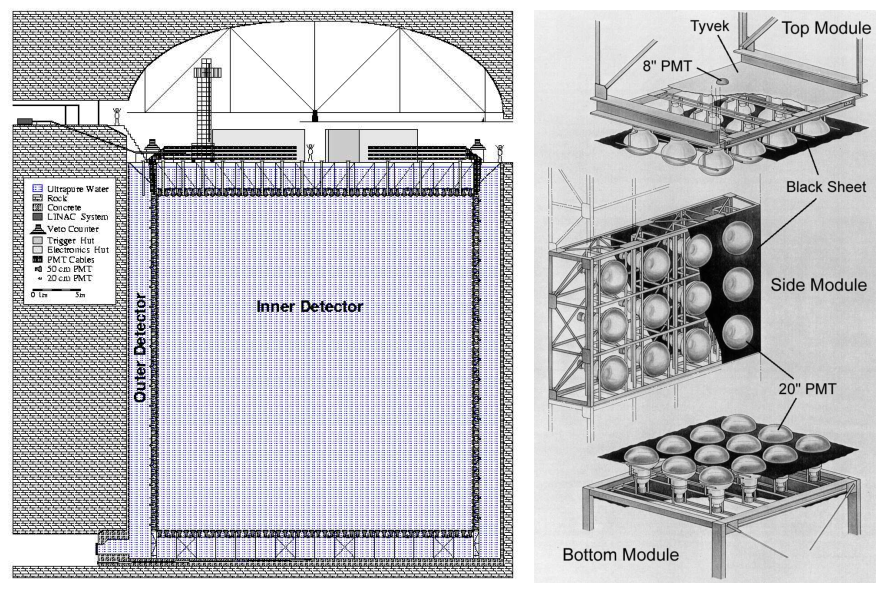
\includegraphics[width=14cm]{Figures/SK/SK_SM}
	\caption[Cross section of the SK detector and overview of supermodule frames]{\label{SK_SK_SM} Cross section of the SK detector (left) and overview of supermodule frames (right)~\cite{2003Fukuda}.}
\end{figure}

\newpage


%
%	Super-Kamiokande
%

\section{Super-Kamiokande}\label{Section_SK}
\Headerfooter{Super-Kamiokande}





\subsection{Super-Kamiokande}
\vs\hs
The Super-Kamiokande (SK)~\cite{2003Fukuda} is the experiment held in Kamioka, Gifu, Japan, with the large water Cherenkov detector placed in 1,000~m underground, 2,700~m water equivalent overburden.
The overview of the SK detector is shown in Figure~\ref{SK_SK}.
The SK stands for ``Super-Kamioka Neutrino Detection Experiment'' and ``Super-Kamioka Nucleon Decay Experiment''.
The rate of cosmic ray muon is reduced by a factor of 10$^{\text{5}}$ compared to that of the ground level.

\begin{figure}[H]
	\centering
	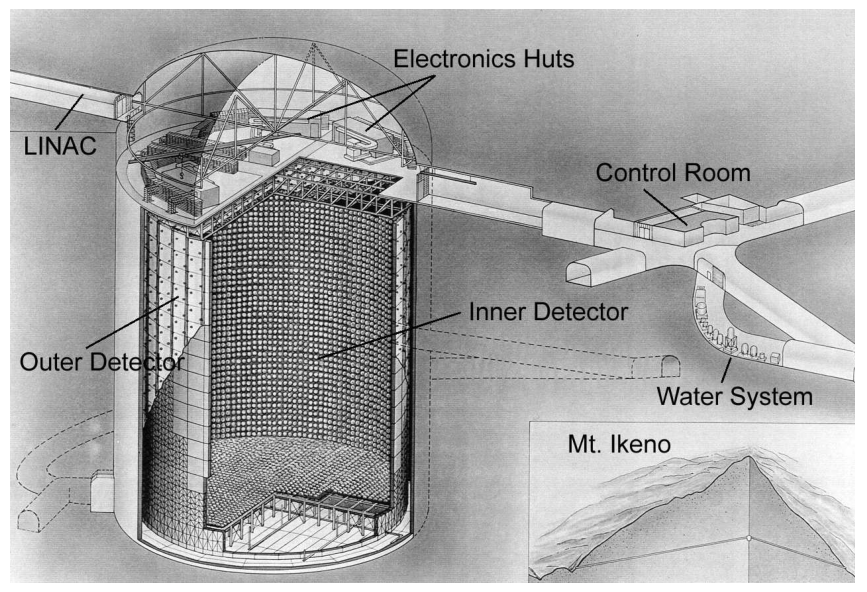
\includegraphics[width=14cm]{Figures/SK/SK}
	\caption[Overview of the Super-Kamiokande detector]{
	Overview of the SK detector~\cite{2003Fukuda}.
	}\label{SK_SK}
\end{figure}

\hs
The SK detector consists of the stainless-steel cylindrical tank with a diameter of 39.3~m and a height of 41.4~m and 50~kilotons ultrapure water.
The tank is separated into the inner detector (ID) and the outer detector (OD) by stainless-steel frames (supermodule frames).
The cross section of the SK detector and the overview of supermodule frames are shown in Figure~\ref{SK_SK_SM}.
The diameter of ID, the height of ID and the volume of ID (the fiducial volume) is 33.8~m, 36.2~m and 32~kilotons (22.5~kilotons), respectively.
In ID, 11,129 20-inch (50~cm) photomultiplier tubes (PMTs) are installed.
The gaps between ID PMTs are covered by black polyethylene terephthalate sheets.
The sheets separate ID and OD optically and suppress the reflection at the surface of the ID wall.
Moreover, the sheets reduce low energy events by radioactive backgrounds occurring behind the PMTs.
On the other hand, in OD, 1,885 8-inch (20~cm) PMTs are installed.
OD volume is covered by white Tyvek sheets manufactured by DuPont.
The Tyvek sheets have high reflectivity and enhance the light collection efficiency in OD.

\begin{figure}[tbp]
	\centering
	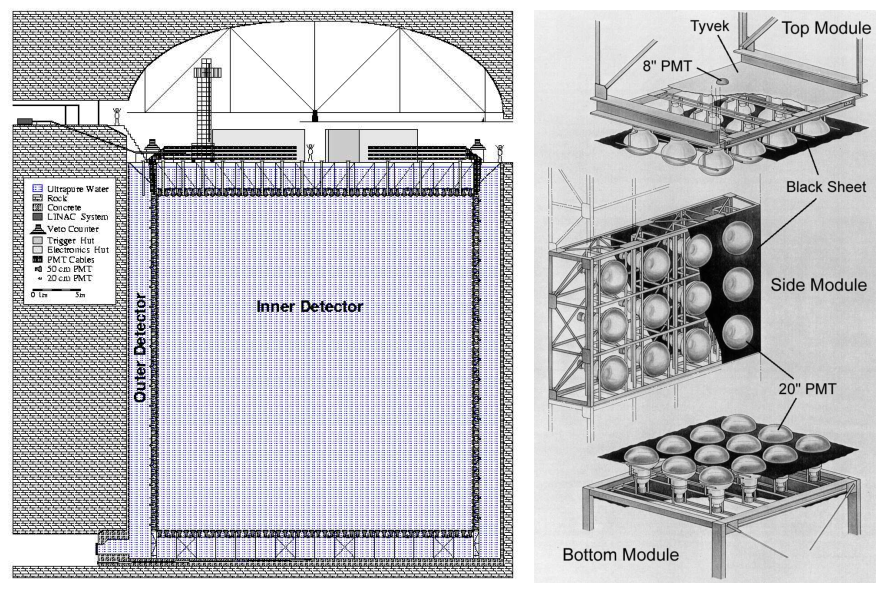
\includegraphics[width=14cm]{Figures/SK/SK_SM}
	\caption[Cross section of the SK detector and overview of supermodule frames]{
	Cross section of the SK detector (left) and overview of supermodule frames (right)~\cite{2003Fukuda}.
	}\label{SK_SK_SM}
\end{figure}





\subsection{ID PMT and OD PMT}
\vs\hs
The schematic view of the ID PMT is shown in Figure~\ref{SK_IDPMT}.
The number of ID PMTs is 7,650 on the barrel (side walls), 1,740 on the top and 1,739 on the bottom, and the effective photocathode coverage of ID is 40\%.
The role of ID PMTs is to reconstruct the energy, generated position, direction and the kind of the charged particles.
Figure~\ref{SK_IDPMTQE} shows the quantum efficiency of the ID PMT photocathode as a function of wavelength.
The material of photocathode is bialkali (Sb-K-Cs) and the quantum efficiency is about 21\% at 360 - 400~nm.
Figure~\ref{SK_IDPMT1pe} shows the single photoelectron pulse height distribution of the ID PMT.
The peak around zero ADC count is caused by PMT dark current.
Figure~\ref{SK_IDPMTt} shows the relative transit time distribution for a typical ID PMT tested using 410~nm wavelength light at the single photoelectron intensity level.
The 1$\sigma$ of transit time for a single photoelectron signal is 2.16~ns.\\
\hs The number of OD PMTs is 1,275 on the barrel, 302 on the top and 308 on the bottom.
To compensate the small number of OD PMTs, wavelength shifting (WS) plate is attached to each OD PMT.
The WS plate is square acrylic panel with a side of 60~cm and a thickness of 1.3~cm, doped with 50~mg$/$L of bis-MSB (C$_{\text{24}}$H$_{\text{22}}$).
The WS plate absorbs UV light, and then emit photons in the blue - green.
OD PMT with bialkali photocathode is more sensitive to blue - green photons than UV photons.
Therefore, the light collection efficiency is improved by about a factor of 1.5 compared to without WS plates.
The timing resolution of OD PMTs with WS plates is 15~ns (FWHM), which is poorer than that of ID PMTs.
However, OD was optimized as a veto counter and the poorer timing resolution is less important.
Figure~\ref{SK_IDODPMT} shows the positional relationship of ID PMTs and OD PMTs in a supermodule frame.
Basically, in a supermodule frame, 12 ID PMTs and 2 OD PMTs are attached.

\begin{figure}[H]
	\centering
	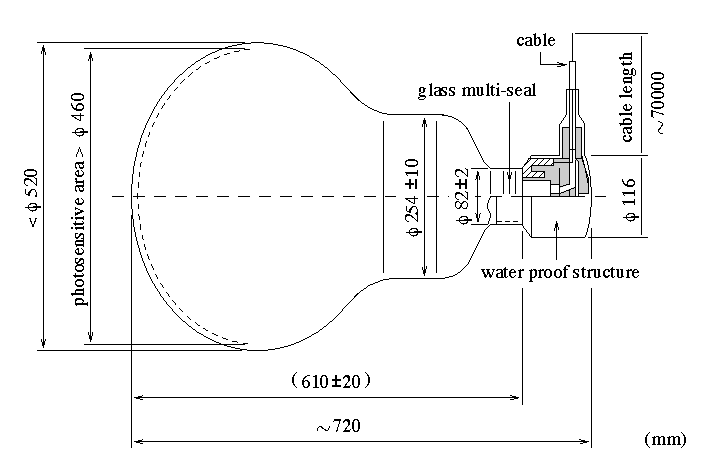
\includegraphics[width=8cm]{Figures/SK/IDPMT}
	\caption[Schematic view of the ID PMT]{
	Schematic view of the ID PMT~\cite{2003Fukuda}.
	}\label{SK_IDPMT}
\end{figure}

\begin{figure}[H]
	\centering
	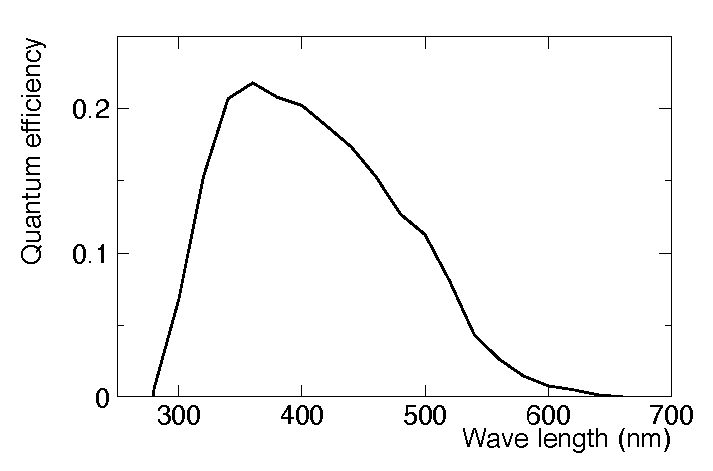
\includegraphics[width=8cm]{Figures/SK/IDPMTQE}
	\caption[Quantum efficiency of the ID PMT photocathode as a function of wavelength]{
	Quantum efficiency of the ID PMT photocathode as a function of wavelength~\cite{2003Fukuda}.
	The material of ID PMT photocathode is bialkali (Sb-K-Cs).
	}\label{SK_IDPMTQE}
\end{figure}

\begin{figure}[H]
	\centering
	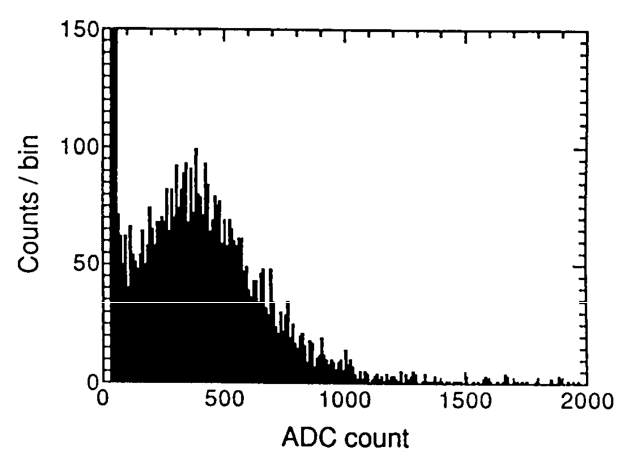
\includegraphics[width=8cm]{Figures/SK/IDPMT1pe}
	\caption[Single photoelectron pulse height distribution of the ID PMT]{
	Single photoelectron pulse height distribution of the ID PMT~\cite{2003Fukuda}.
	The peak around zero ADC count is caused by PMT dark current.
	}\label{SK_IDPMT1pe}
\end{figure}

\begin{figure}[H]
	\centering
	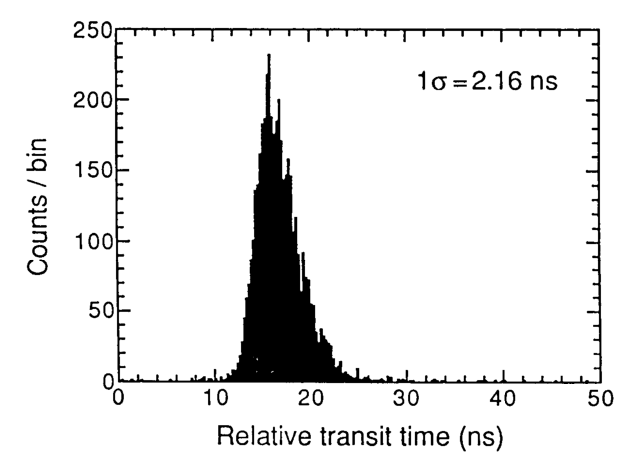
\includegraphics[width=8cm]{Figures/SK/IDPMTt}
	\caption[Relative transit time distribution for a typical ID PMT tested using 410~nm wavelength light at the single photoelectron intensity level]{
	Relative transit time distribution for a typical ID PMT tested using 410~nm wavelength light at the single photoelectron intensity level~\cite{2003Fukuda}.
	}\label{SK_IDPMTt}
\end{figure}

\begin{figure}[H]
	\centering
	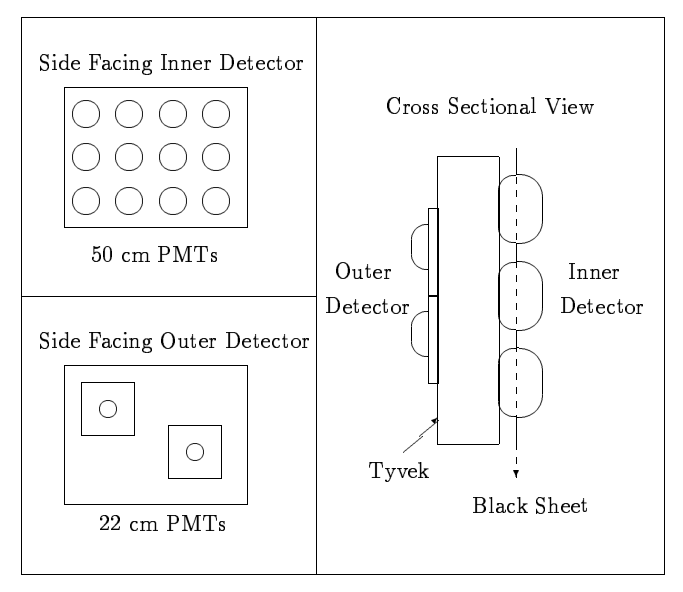
\includegraphics[width=10cm]{Figures/SK/IDODPMT}
	\caption[Positional relationship of ID PMTs and OD PMTs in a supermodule frame]{
	Positional relationship of ID PMTs and OD PMTs in a supermodule frame~\cite{1997ZoaPhD}.
	12 ID PMTs and 2 OD PMTs are attached in a supermodule frame, basically.
	}\label{SK_IDODPMT}
\end{figure}





\subsection{Helmholtz coils}
\vs\hs
The geomagnetic field would affect photoelectron trajectories and timing in the PMTs.
Therefore, 26 sets of horizontal and vertical Helmholtz coils are deployed around the inner surface of the tank to reduce the geomagnetic field.
Figure~\ref{SK_Coil} shows the schematic view of Helmholtz coils.
The average geomagnetic field intensity without Helmholtz coils is about 450~mG~\cite{2003Fukuda}.
The average field intensity can be reduced to 32~mG with Helmholtz coils, resulting that the deviation in the collection efficiency of photoelectrons is 2\%~\cite{2014AbeCalib}.

\begin{figure}[H]
	\centering
	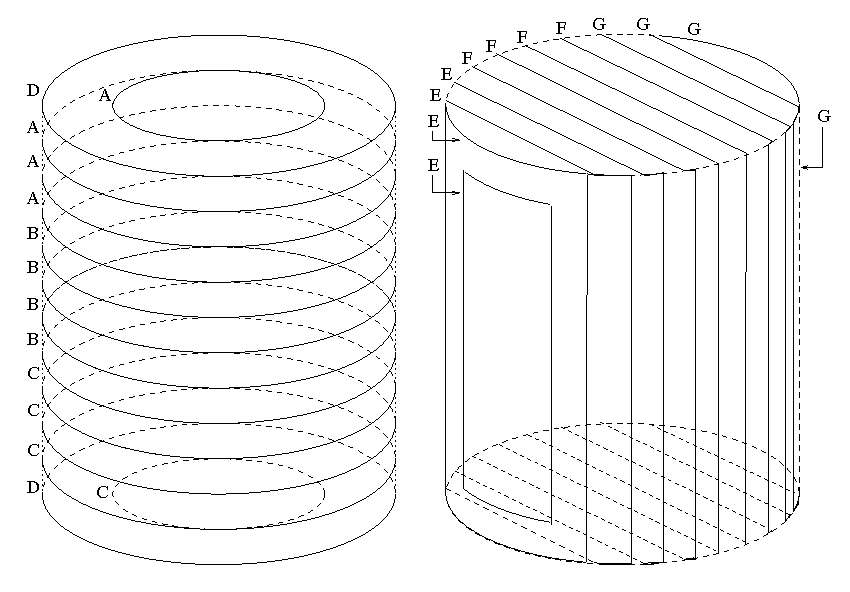
\includegraphics[width=12cm]{Figures/SK/Coil}
	\caption[Schematic view of Helmholtz coils]{
	Schematic view of Helmholtz coils~\cite{1998YamaguchiPhD}.
	}\label{SK_Coil}
\end{figure}





\subsection{Observation phase}\label{SK_Obs_pha}
\vs\hs
The observation phase of SK is categorized into seven, from SK-I to SK-VII.
Each observation phase is described below.\\
\\
\textbf{SK-I}\\
\hs
SK-I started in April 1996 and ended in July 2001.
In ID, 11,146 PMTs were attached and the effective photocathode coverage of ID was 40\%.
It was during the SK-I that we got the evidence for neutrino oscillation~\cite{1998Fukuda}.\\
\\
\textbf{SK-II}\\
\hs
In November 12th, 2001, one bottom PMT broke when ultrapure water was filled into SK detector after finishing the detector maintenance.
Due to the shockwave generated at that time, other PMTs were broken in a chain.
As a result, it became a serious accident that 6,779 ID PMTs and 1,017 OD PMTs were lost.
In SK-II, which started in October 2002 and ended in October 2005, the observation was performed using 5,182 remained and spare ID PMTs and 1,885 remained and new OD PMTs.
The effective photocathode coverage of ID was 19\%.
Since SK-II, each ID PMT has been covered with a shockwave prevention case.
The case consists of an acrylic that covers the photocathode and Fiber Reinforced Plastic (FRP) case that covers parts other than the photocathode.
The case not only prevents shockwave but also increases the water pressure resistance of the PMT.
The picture of a shockwave prevention case is shown in Figure~\ref{SK_Case}.\\

\begin{figure}[tbp]
	\centering
	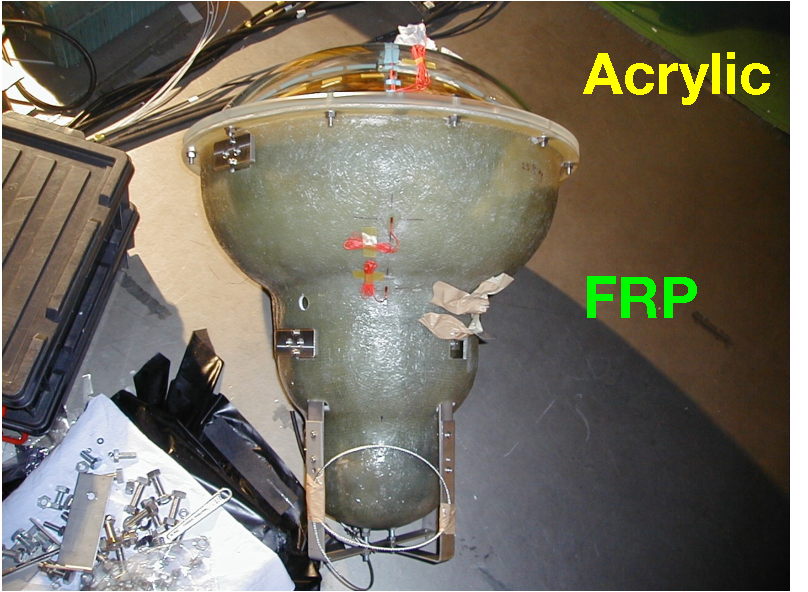
\includegraphics[width=8cm]{Figures/SK/Case}
	\caption[Picture of a shockwave prevention case]{
	Picture of a shockwave prevention case~\cite{SKaccident}.
	}\label{SK_Case}
\end{figure}

\textbf{SK-III}\\
\hs
SK-III started in July 2006 and ended in August 2008.
Since SK-III, the number of ID PMTs has been 11,129 and the effective photocathode coverage of ID has been 40\%.
The reason why the number of ID PMTs is reduced by 17 compared to SK-I is that ID PMTs cannot be installed at the edge of the detector because the size of the shockwave prevention case is large.\\
\\
\textbf{SK-IV}\\
\hs
In September 2008, the data acquisition system was renewed from Analog Timing Module (ATM) to QTC-Based Electronics with Ethernet (QBEE) and SK-IV started~\cite{2009Nishino}.
QTC stands for charge-to-time converter.
The renewal of the system allows us to open the data acquisition time window until 535~$\mu$s (385~$\mu$s before November 2010~\cite{2021Abe}) from the trigger timing and enabled to search neutron signals~\cite{2009Watanabe}.
SK-IV continued until June 2018 and is longest phase at this time.\\
\\
\textbf{SK-V}\\
\hs
The tank refurbishment work toward the SK-Gd experiment was conducted between SK-IV and SK-V.
The purpose of the work was the water stop reinforcement of the tank, the piping improvement in the tank and the PMT replacement.
After finishing the work, SK-V started in January 2019 and ended in July 2020.\\
\\
\textbf{SK-VI}\\
\hs
In July 2020, we dissolved 13.2~tons of Gd$_{\text{2}}$(SO$_{\text{4}}$)$_{\text{3}}\,\cdot\,$8H$_{\text{2}}$O (we introduced 0.011\% of Gd) into the SK tank and SK-VI (the SK-Gd experiment) started.
Since Gd has the largest thermal neutron capture cross section among natural elements, neutron capture rate on Gd is high even at low concentrations.
Table~\ref{SK_Tab:ThermalNeutron} and Figure~\ref{SK_Gd_capture_rate} show the thermal neutron capture cross sections~\cite{2022MarkSlide} and neutron capture rate on Gd~\cite{2020Marti}, respectively.
Moreover, when a thermal neutron is captured on Gd, a total of about 8~MeV of gamma-rays are emitted.
From these reasons, neutron-tagging efficiency is largely improved in SK-Gd.
The time constant of neutron capture at this Gd mass concentration is about 115~$\mu$s~\cite{2022Abe}.
SK-VI continued until June 2022.\\

\begin{table}[H]
	\caption[Thermal neutron capture cross sections]{
	Thermal neutron capture cross sections~\cite{2022MarkSlide}.
	}\label{SK_Tab:ThermalNeutron}
	\centering
	\vs
	\begin{tabular}{lrrrr} \hline\hline
		                                          & H    & O      & S    & Gd     \\ \hline
		Thermal neutron capture cross section [b] & 0.33 & 0.0002 & 0.53 & 49,700 \\ \hline\hline
	\end{tabular}
\end{table}

\begin{figure}[H]
	\centering
	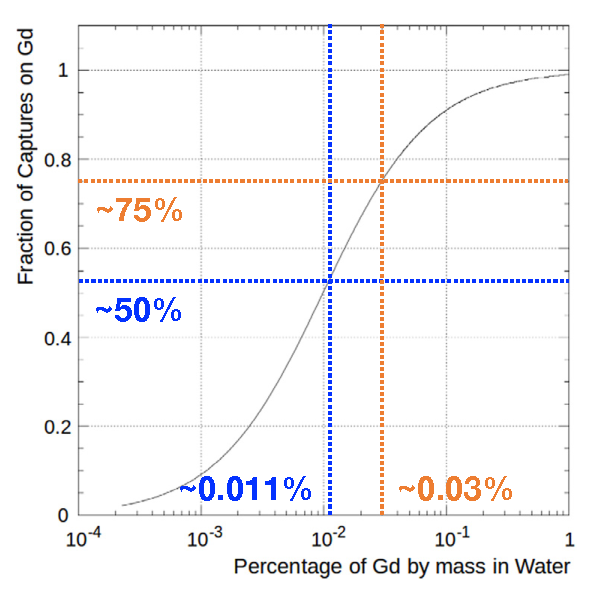
\includegraphics[width=8cm]{Figures/SK/Gd_capture_rate}
	\caption[Neutron capture rate on Gd]{
	Neutron capture rate on Gd~\cite{2020Marti}.
	}\label{SK_Gd_capture_rate}
\end{figure}

\textbf{SK-VII}\\
\hs
In June 2022, we additionally dissolved 27.3~tons of Gd$_{\text{2}}$(SO$_{\text{4}}$)$_{\text{3}}\,\cdot\,$8H$_{\text{2}}$O into the SK tank and SK-VII started.
The Gd mass concentration is comparable to 0.03\%.
The time constant of neutron capture at this Gd mass concentration is about 62~$\mu$s.\\
\\
\hs
The information of each observation phase is summarized in Table~\ref{SK_Tab:phase}.

\begin{table}[h]
	\caption[Information of each observation phase]{
	Information of each observation phase.
	}\label{SK_Tab:phase}
	\centering
	\vs
	\begin{tabular}{lrrr} \hline\hline
		Phase                    & SK-I          & SK-II        & SK-III        \\ \hline
		Start                    & Apr. 1996     & Oct. 2002    & Jul. 2006     \\
		End                      & Jul. 2001     & Oct. 2005    & Sep. 2008     \\
		\# of ID PMTs (Coverage) & 11,146 (40\%) & 5,182 (19\%) & 11,129 (40\%) \\
		\# of OD PMTs            & 1,885         & 1,885        & 1,885         \\
		Electronics              & ATM           & ATM          & ATM           \\
		Gd mass concentration    & 0\%           & 0\%          & 0\%           \\ \hline\hline
	\end{tabular}
	\\
	\vs\vs
	\begin{tabular}{lrrrr} \hline\hline
		Phase                    & SK-IV         & SK-V          & SK-VI         & SK-VII        \\ \hline
		Start                    & Sep. 2008     & Jan. 2019     & Jul. 2020     & Jun. 2022     \\
		End                      & Jun. 2018     & Jul. 2020     & Jun. 2022     & -             \\
		\# of ID PMTs (Coverage) & 11,129 (40\%) & 11,129 (40\%) & 11,129 (40\%) & 11,129 (40\%) \\
		\# of OD PMTs            & 1,885         & 1,885         & 1,885         & 1,885         \\
		Electronics              & QBEE          & QBEE          & QBEE          & QBEE          \\
		Gd mass concentration    & 0\%           & 0\%           & 0.011\%       & 0.03\%        \\ \hline\hline
	\end{tabular}
\end{table}





\subsection{Detection principle}\label{subsec_detect_princi}
\vs\hs
When the speed of the charged particle passing through the dielectric medium is faster than the speed of light in the medium, photons are radiated conically along the track of the particle.
This phenomenon is called ``Cherenkov radiation'', and the radiated photons are called ``Cherenkov photons''.
Figure~\ref{SK_Cherenkov_03} shows the schematic view of Cherenkov radiation.
The Cherenkov photons are projected in a ring as shown in left side of Figure~\ref{SK_Cherenkov_03}.
The ring is called ``Cherenkov ring''.
In the SK, the energy, generated position, direction and the kind of the charged particle are reconstructed using the time, quantity of charge and Cherenkov ring pattern information that ID PMTs received.
In right side of Figure~\ref{SK_Cherenkov_03}, the charged particle with velocity $v$ moves distance $vt={v \over c}ct=\beta ct$ in time $t$, where $c$ is the speed of light in vacuum and $\beta={v \over c}$ is the ratio of $v$ and $c$.
While the Cherenkov photon moves distance ${c \over n}t$ in time $t$, where $n$ is the refractive index of the dielectric medium.
Therefore, when the angle between the direction of charged particle and the direction of Cherenkov photon is defined as $\theta_{{\rm C}}$, the next formula is established,
\begin{eqnarray}\label{SK_Eq_Che}
	\cos\theta_{{\rm C}}={{c \over n}t \over \beta ct}={1 \over n\beta}.
\end{eqnarray}
In Equation (\ref{SK_Eq_Che}), assuming that $n=1.34$, which is the refractive index of water, and $\beta=1$, $\theta_{{\rm C}}$ becomes about 42~degrees.
Therefore, in water, the maximum angle between the direction of charged particle and the direction of Cherenkov angle is about 42~degrees.\\
\hs
The energy $E$ required for the charged particle with rest mass $m$ to emit Cherenkov photons (Cherenkov threshold) is
\begin{eqnarray}
	E={mc^{2} \over \sqrt{1-\beta^{2}}}\geq{mc^{2} \over \sqrt{1-\Big({1 \over n}\Big)^{2}}}={nmc^{2} \over \sqrt{n^{2}-1}}.
\end{eqnarray}
The Cherenkov threshold of main charged particles is summarized in Table~\ref{SK_Tab:Che}.\\
\hs
Assuming that the wavelength region of Cherenkov photons is from $\lambda_{1}$ to $\lambda_{2}$, the number of Cherenkov photons $N$ emitted per unit length $x$ when the particle with charge $z$ passes through the medium is
\begin{eqnarray}
	{dN \over dx}=2\pi\alpha z^{2}\sin ^{2} \theta_{{\rm C}}\bigg({1 \over \lambda_{1}}-{1 \over \lambda_{2}}\bigg),
\end{eqnarray}
where $\alpha$ is the fine-structure constant.

\begin{figure}[H]
	\centering
	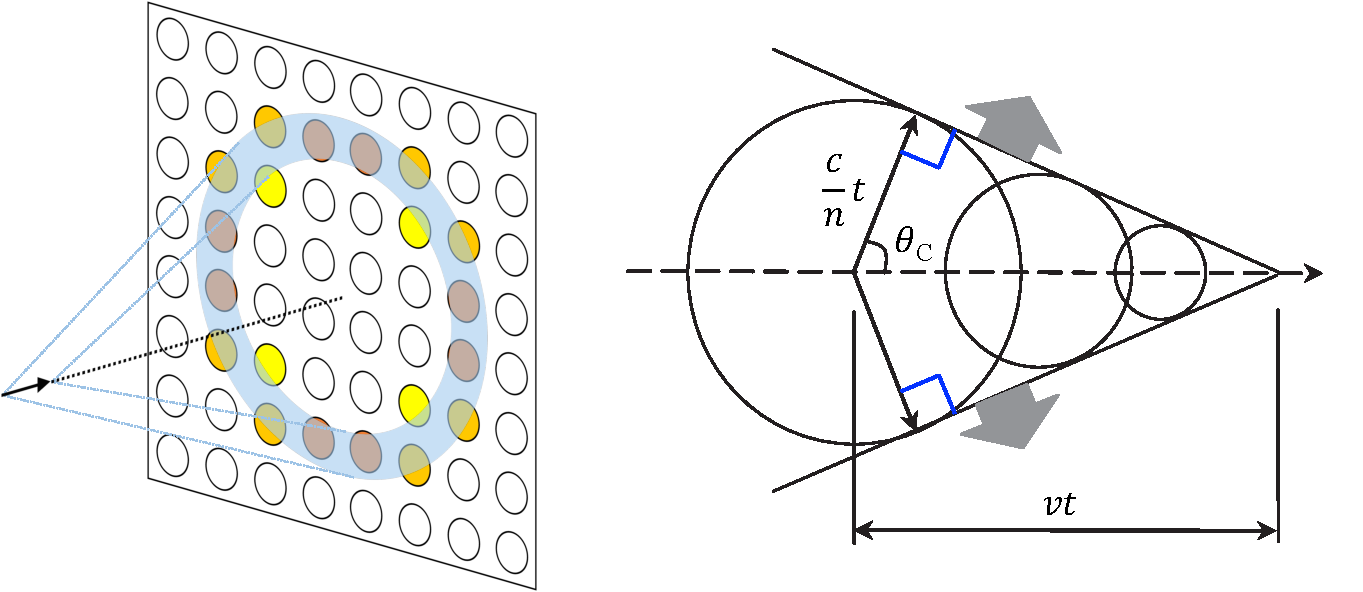
\includegraphics[width=14cm]{Figures/SK/Cherenkov_03}
	\caption[Schematic view of Cherenkov radiation]{
	Schematic view of Cherenkov radiation~\cite{2015Yamamoto}.
	}\label{SK_Cherenkov_03}
\end{figure}

\begin{table}[H]
	\caption[Cherenkov threshold of main charged particles]{
	Cherenkov threshold of main charged particles~\cite{2022Workman}.
	$m$ is rest mass and $E$ is Cherenkov threshold.
	Here $n=1.34$ is assumed.
	}\label{SK_Tab:Che}
	\centering
	\vs
	\begin{tabular}{lrrrrr} \hline\hline
		Charged particle  & e$^{\pm}$ & $\mu^{\pm}$ & $\pi^{\pm}$ & K$^{\pm}$ &p         \\ \hline
		$m$~[MeV$/c^{2}$] & 0.511     & 105.658     & 139.570     & 493.677   &938.272   \\
		$E$~[MeV]         & 0.768     & 158.730     & 209.676     & 741.652   &1,409.568 \\ \hline\hline
	\end{tabular}
\end{table}





\subsection{Water purification system}\label{Section_WaterPuri}
\vs\hs
The 50 kilotons ultrapure water of the SK is made from the underground water of the Kamioka mine.
The underground water contains the dust, bacteria and radioactive impurities.
These impurities should be removed to avoid decreasing the water transparency and increasing low energy backgrounds.
In the SK, these impurities are removed by circulating and purifying the ultrapure water using the water purification system at a flow rate of 120~m$^{\text{3}}/$h.
Figure~\ref{SK_Water} shows the schematic view of water purification system.
This system consists of three systems: the dissolving system, the pretreatment system and the re-circulation system.
The dissolving system and the pretreatment system are used during Gd loading, while the re-circulation system is used during both Gd loading and data taking.
Here each component of re-circulation system is described below.
\begin{itemize}
	\item UV total organic carbon reduction lamp (TOC): TOC lamp oxidatively decomposes carbon and other compounds. These are eventually decomposed into water and carbon dioxide.
	\item Heat exchanger (HE): High water temperature causes the bacterial growth, the decrease of water transparency and the increase of PMT dark noise. HE keeps the water temperature around 13~$^{\circ}$C at a precision better than 0.01~$^{\circ}$C.
	\item Strongly acidic cation exchange resin (C-Ex Resin): C-Ex Resin removes positively charged impurities, and radium ions in particular, while preserving the dissolved gadolinium ions (Gd$^{\text{3}+}$).
	\item Strongly basic anion exchange resin (A-Ex Resin): A-Ex Resin removes negatively charged impurities while preserving the dissolved sulfate ions (SO$^{\text{2}-}_{\text{4}}$).
	\item One micron filter (1~$\mu$m): 1~$\mu$m filter removes the dusts larger than 1~$\mu$m.
	\item UV sterilizer (UV): UV sterilizer kills the bacteria.
	\item Ultrafiltration modules (UF): UF modules remove tiny dusts.
	\item Membrane degasifier (MD): MD removes radon dissolved in the ultrapure water.
\end{itemize}

\begin{figure}[H]
	\centering
	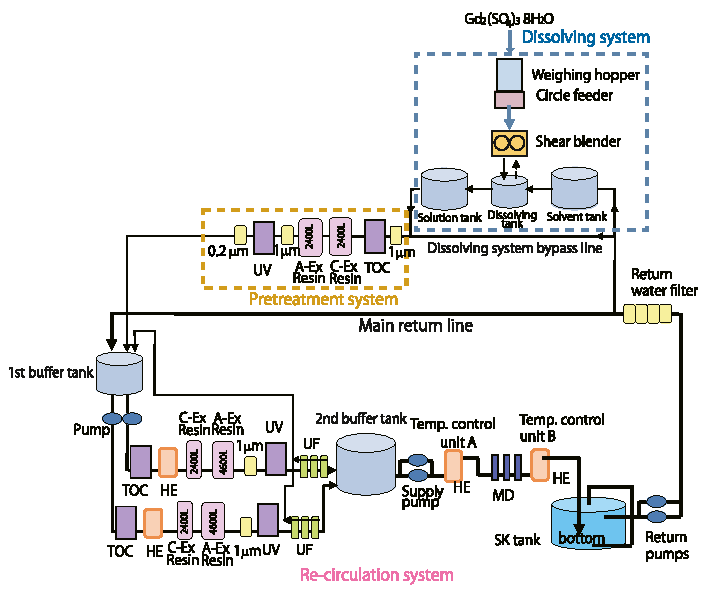
\includegraphics[width=14cm]{Figures/SK/Water}
	\caption[Schematic view of water purification system]{
	Schematic view of water purification system~\cite{2022Abe}.
	The dissolving system and the pretreatment system are used during Gd loading, while the re-circulation system is used during both Gd loading and data taking.
	}\label{SK_Water}
\end{figure}





\subsection{Air purification system}
\vs\hs
Most of radioactive backgrounds come from radon, which is rich in the rock of the Kamioka mine.
To reduce radioactive backgrounds, radon in the air should be reduced as much as possible.\\
\hs
Figure~\ref{SK_AirSeason} shows the typical radon concentration in the air at the SK over a year.
Radon concentration in the air of the mine is 2,000 - 3,000~Bq$/$m$^{\text{3}}$ during the warm season, from May to October, while the concentration is 100 - 300~Bq$/$m$^{\text{3}}$ in the cold season, from November to April.
This is because the airflow inside the mine changes depending on the temperature outside the mine.
To keep the concentration below 100~Bq$/$m$^{\text{3}}$ inside the experimental area, fresh air is continuously blown at a flow rate of 10~m$^{\text{3}}/$min from outside the mine (Radon Hut) to the experimental area through an air duct.
The flow rate makes the air pressure inside the experimental area higher than outside, minimizing the entry of the air outside the experimental area.
As a result, the concentration inside the experimental area is kept at 30 - 50~Bq$/$m$^{\text{3}}$ throughout the year, as shown in Figure~\ref{SK_AirSeason}.\\
\hs
However, the radon concentration inside the experimental area is still too high for observations with low radioactive backgrounds.
Therefore, the fresh air is purified using the air purification system, then the purified air is supplied to the gap between the top of the SK tank and the water surface.
Figure~\ref{SK_Air} shows the schematic view of air purification system.
Each component of air purification system is described in Ref.~\cite{2015NakanoPhD}.
The residual radon concentration in the purified air is a few~mBq$/$m$^{\text{3}}$.

\begin{figure}[H]
	\centering
	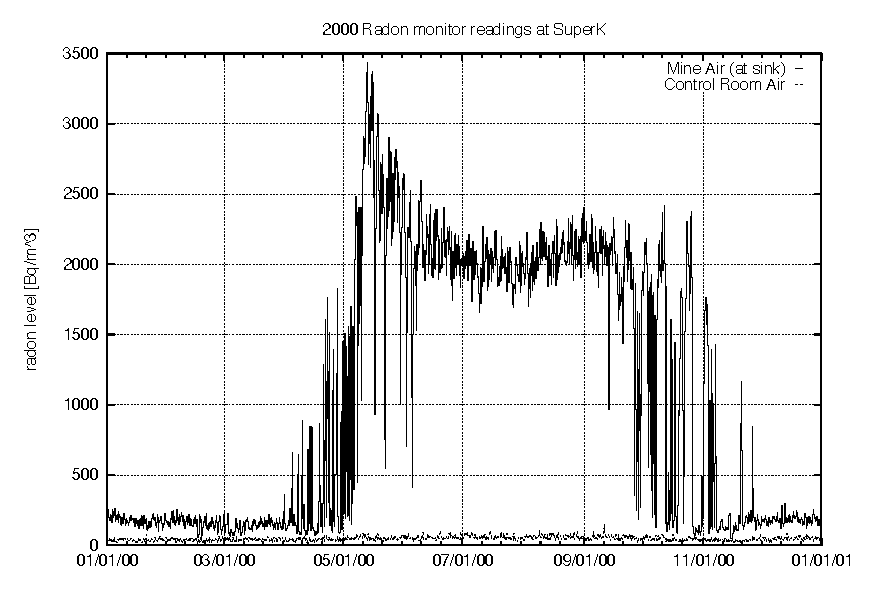
\includegraphics[width=10cm]{Figures/SK/AirSeason}
	\caption[Typical radon concentration in the air at the SK over a year]{
	Typical radon concentration in the air at the SK over a year~\cite{2003Fukuda}.
	The solid line shows the concentration outside the experimental area.
	The dashed line shows the concentration inside the experimental area.
	}\label{SK_AirSeason}
\end{figure}

\begin{figure}[H]
	\centering
	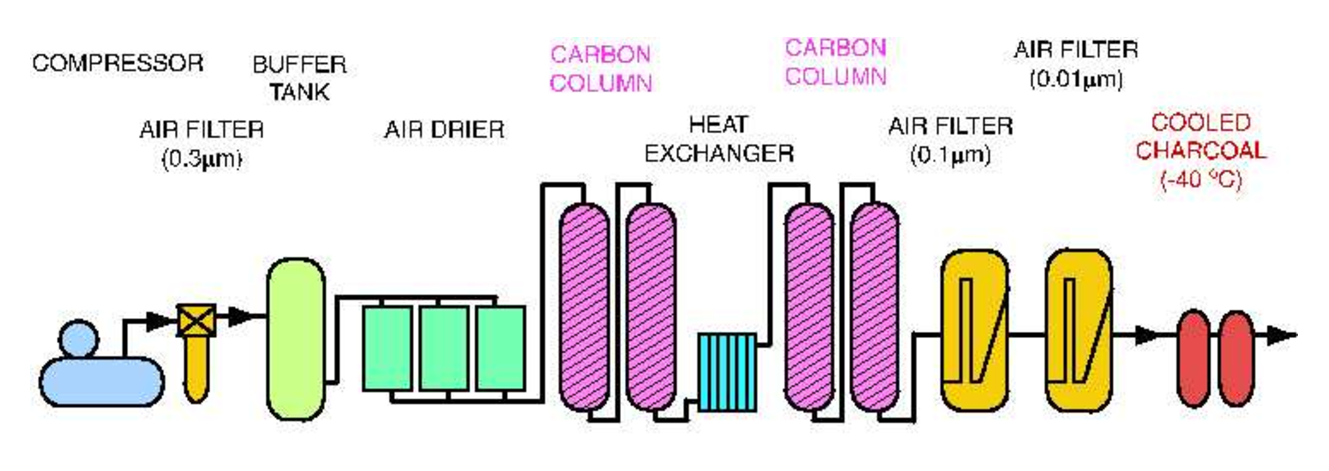
\includegraphics[width=12cm]{Figures/SK/Air}
	\caption[Schematic view of air purification system]{
	Schematic view of air purification system~\cite{2003Fukuda}.
	Each component of air purification system is described in Ref.~\cite{2015NakanoPhD}.
	}\label{SK_Air}
\end{figure}





\subsection{Data acquisition system}\label{subsec_data_acqu}
\vs\hs
As explained in Section~\ref{SK_Obs_pha}, the data acquisition system was changed from ATM to QBEE in SK-IV.
The data used in this thesis was acquired by QBEE.
Therefore, the description of ATM is omitted in this thesis.\\
\hs
Figure~\ref{SK_DAQ} shows the schematic view of the data acquisition system after SK-IV.
One QBEE board has 8 QTCs, and one QTC has 3 analog input channels for PMT signals.
That is, one QBEE board has 24 analog input channels for PMT signals.
Figure~\ref{SK_QTC} shows the block diagram of the QTC and its surroundings.
Each analog input channel has three gain ranges: small, medium, and large.
The gain ratio of small, medium, and large is set to 1, 1$/$7, and 1$/$49, respectively.
Also, the charge dynamic range of small, medium, and large is 0.2 - 51~pC, 1 - 357~pC, and 5 - 2500~pC, respectively.
The gain ratio is optimized to cover a wide charge dynamic range with reasonable resolution.
When the charge is sent to a QBEE board, the QTC integrates the charge and generates the output signal with the width proportional to the integrated charge.
Then the output signal is digitized by time-to-digital converter (TDC).
The digitized signals are transferred to 20 front-end PCs, and sent to 10 merger PCs.
In the merger PCs, the signals from all the front-end PCs are merged and the software trigger is applied.
Details about the software trigger is described later.
From the merger PCs, signals for triggered events are sent to an organizer PC and then written onto the disk for offline analysis.
Details about the front-end PCs, merger in the merger PCs, the organizer PC, and the disk are described in Ref.~\cite{2010Yamada}.\\
\hs
The software trigger process scans the signals sent to the merger PCs and searches the events satisfying the trigger conditions.
A trigger is applied when the number of ID PMT hits within 200~ns, which corresponds to the time that a Cherenkov photon moves from the edge of the SK tank to other, is a certain value or more.
Figure~\ref{SK_softtrg_SK4} and Figure~\ref{SK_softtrg_SK567} show the software trigger threshold for recording PMT hits of each trigger type from SK-IV to SK-VII.
%Table~\ref{SK_Tab:Tri} shows the trigger threshold and time width for recording PMT hits of each trigger type in SK-VI.
There are four trigger types for ID: Super Low Energy (SLE), Low Energy (LE), High Energy (HE), and Super High Energy (SHE).
Each trigger threshold changes depending on its trigger rate.
Also, OD trigger is applied when the number of OD PMT hits within 200~ns is 22 or more.
Basically, when a trigger is applied, all hits from $-$5~$\mu$s to 35~$\mu$s are recorded, where the trigger timing is 0~$\mu$s.
However, in the case of SLE, all hits from $-$0.5~$\mu$s to 1.0~$\mu$s are recorded due to the high trigger rate.\\
\hs
From SK-IV, a special trigger, AFT, was installed to search delayed neutron capture signals.
Previously, AFT trigger was applied when SHE trigger was applied and OD trigger was not applied to avoid events by cosmic ray muons.
However, from June 2020, the condition about OD trigger was removed to study spallation events by cosmic ray muons.
When AFT trigger is applied, all hits from 35~$\mu$s to 535~$\mu$s (from 35~$\mu$s to 385~$\mu$s before November 2010~\cite{2021Abe}) in addition to from $-$5~$\mu$s to 35~$\mu$s are recorded.

\begin{figure}[h]
	\centering
	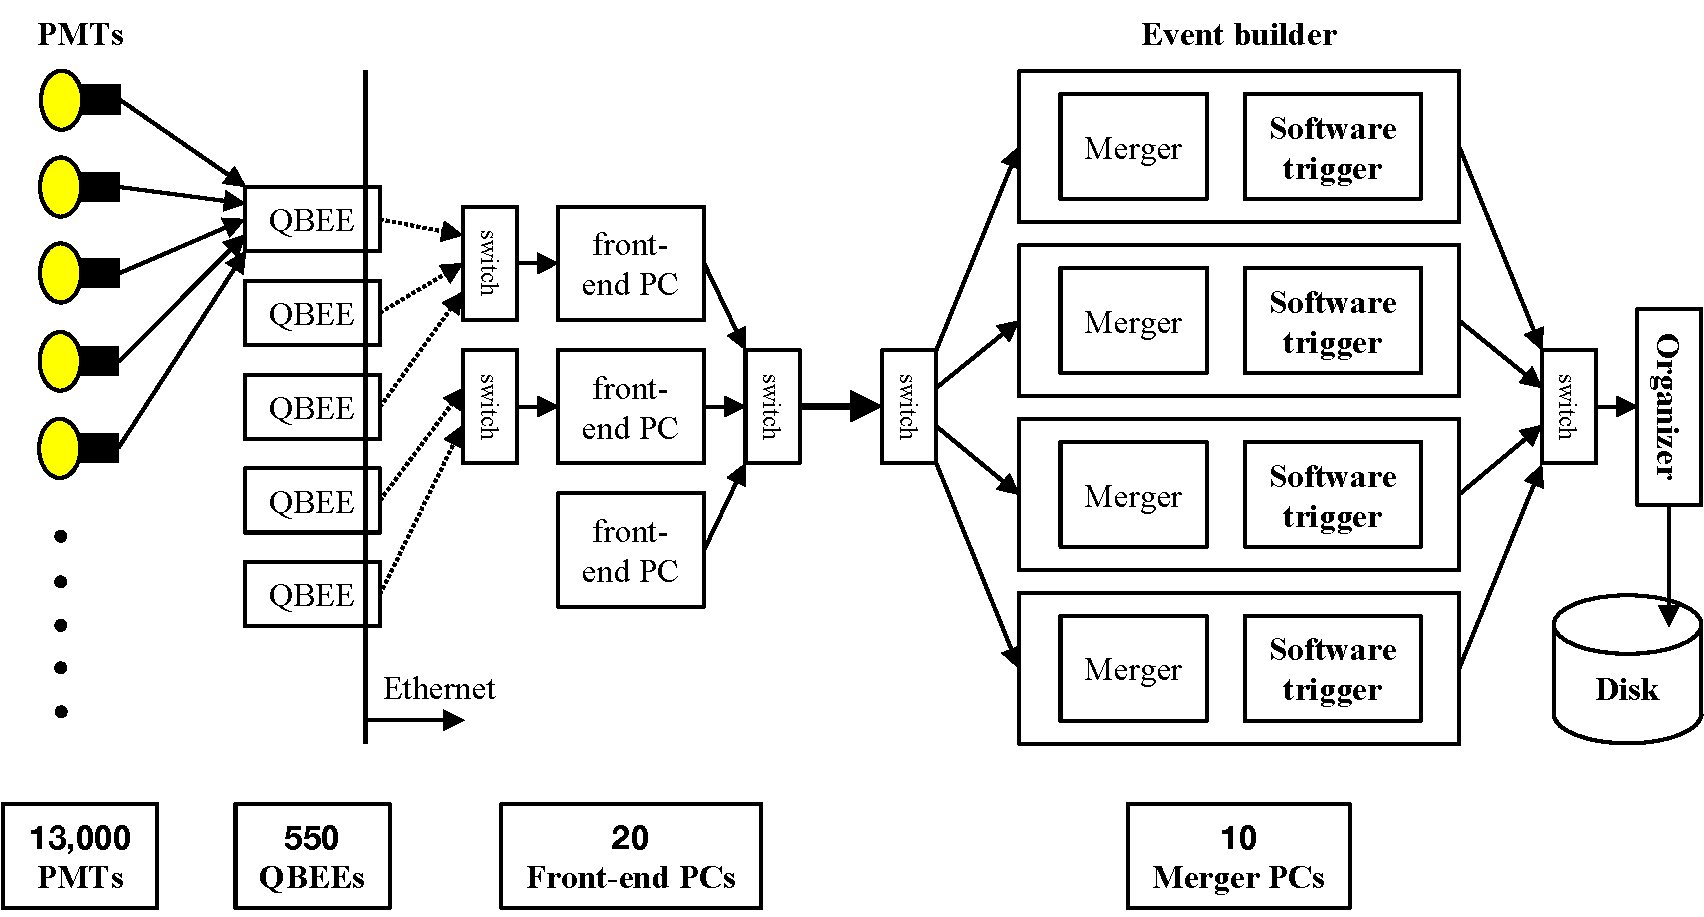
\includegraphics[width=12cm]{Figures/SK/DAQ}
	\caption[Schematic view of the data acquisition system]{
	Schematic view of the data acquisition system~\cite{2010Yamada}.
	}\label{SK_DAQ}
\end{figure}

\begin{figure}[h]
	\centering
	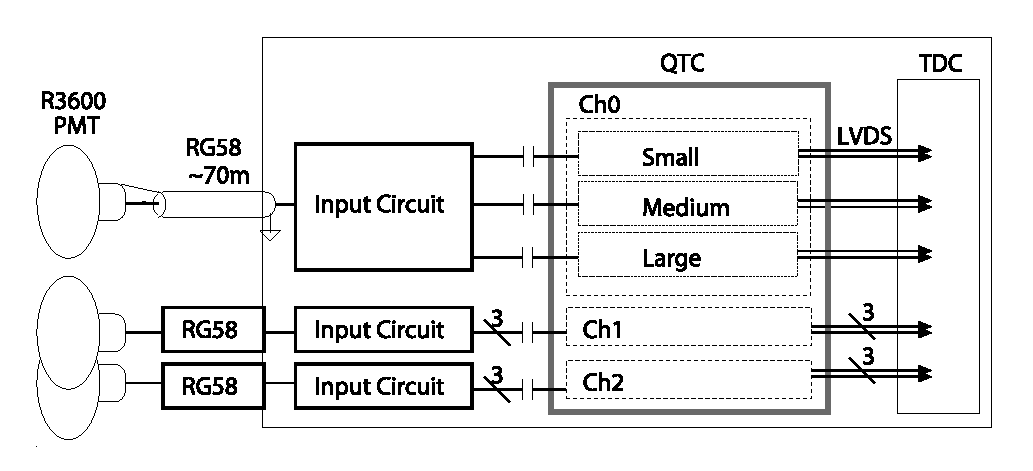
\includegraphics[width=12cm]{Figures/SK/QTC}
	\caption[Block diagram of the QTC and its surroundings]{
	Block diagram of the QTC and its surroundings~\cite{2009Nishino}.
	The output signal of each range (small, medium, or large) is generated by low voltage differential signaling (LVDS) drivers and digitized by time-to-digital converter (TDC).
	}\label{SK_QTC}
\end{figure}

%\begin{table}[h]
%	\caption[Trigger threshold and time width for recording PMT hits of each trigger type in SK-VI]{
%	Trigger threshold and time width for recording PMT hits of each trigger type in SK-VI.
%	$N_{200,\,{\rm ID}}$ and $N_{200,\,{\rm OD}}$ shows the number of ID or OD PMT hits within 200 ns.
%	}\label{SK_Tab:Tri}
%	\centering
%	\vs
%	\begin{tabular}{ccc} \hline\hline
%		Trigger type & Trigger threshold          & Time width [$\mu$s] \\ \hline
%		SLE          & $N_{200,\,{\rm ID}}\ge$ 34 & 1.5                 \\
%		LE           & $N_{200,\,{\rm ID}}\ge$ 49 & 40                  \\
%		HE           & $N_{200,\,{\rm ID}}\ge$ 52 & 40                  \\
%		SHE          & $N_{200,\,{\rm ID}}\ge$ 60 & 40                  \\
%		OD           & $N_{200,\,{\rm OD}}\ge$ 22 & 40                  \\ \hline\hline
%	\end{tabular}
%\end{table}

\begin{figure}[h]
	\centering
	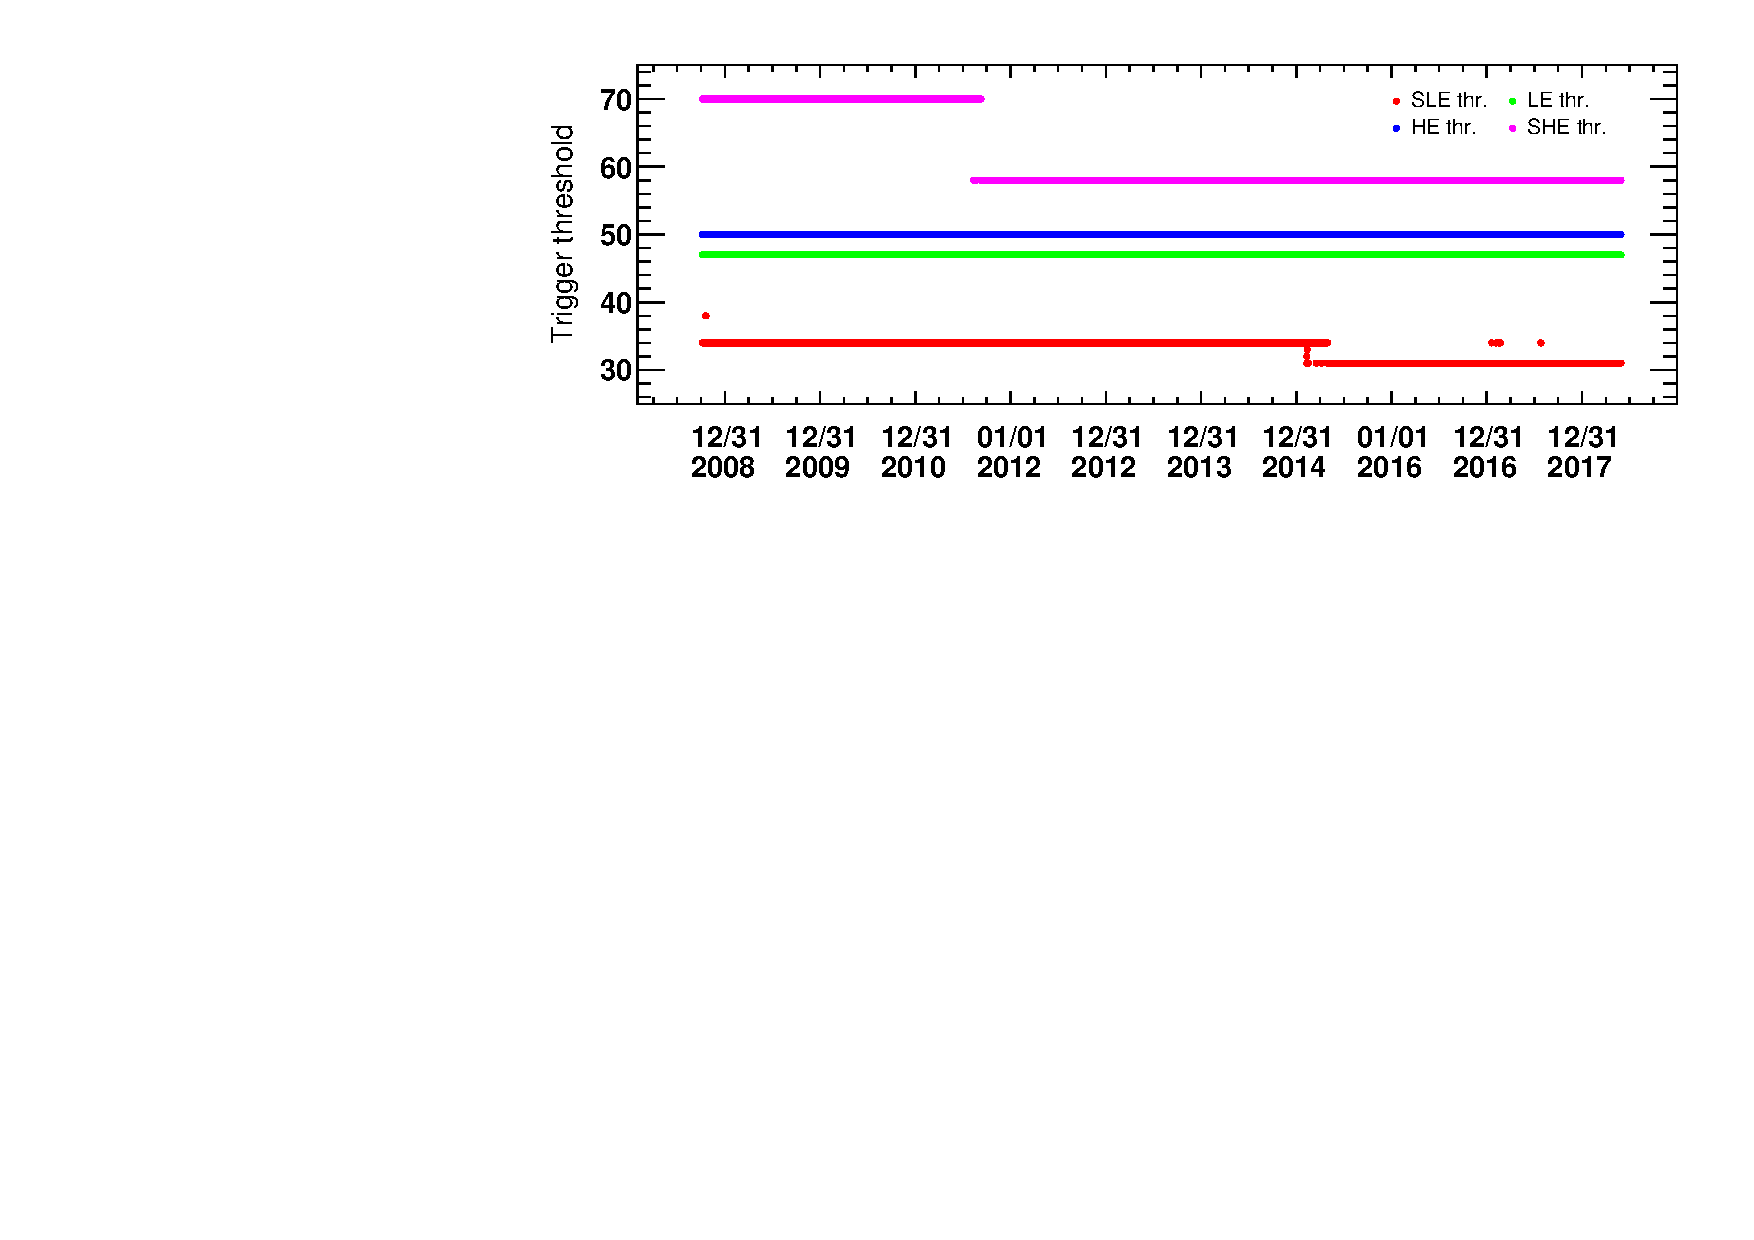
\includegraphics[width=15cm]{Figures/SK/softtrg_thr_time_vari_SK4}
	\caption[Software trigger threshold for recording PMT hits of each trigger type in SK-IV]{
	Software trigger threshold for recording PMT hits of each trigger type in SK-IV.
	After May 2015, SLE trigger threshold changed from 34 to 31.
	While, after September 2011, SHE trigger thershold changed from 70 to 58.
	During SK-IV, LE and HE trigger threshold was 47 and 50, respectively.
	}\label{SK_softtrg_SK4}
\end{figure}

\begin{figure}[h]
	\centering
	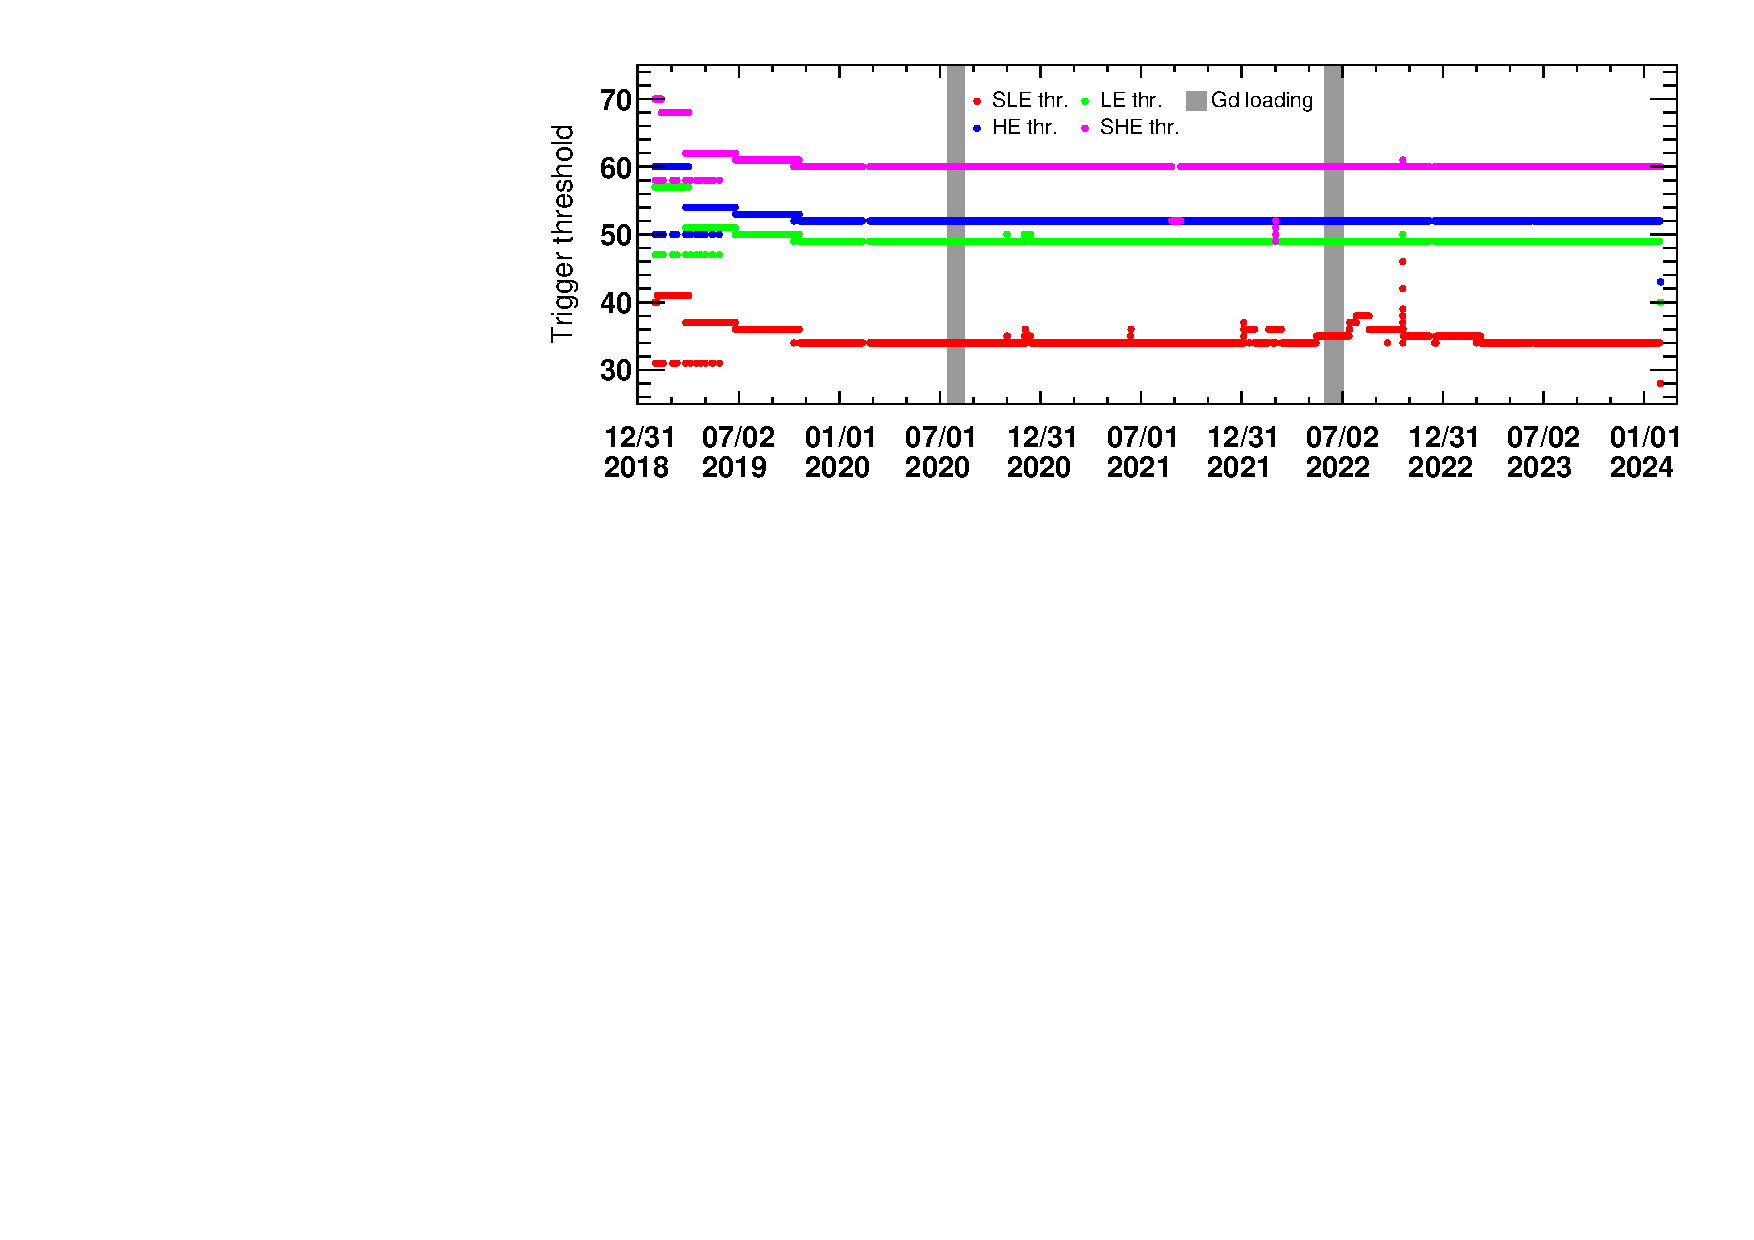
\includegraphics[width=15cm]{Figures/SK/softtrg_thr_time_vari_SK567}
	\caption[Software trigger threshold for recording PMT hits of each trigger type in SK-V, SK-VI, and SK-VII]{
	Software trigger threshold for recording PMT hits of each trigger type in SK-V, SK-VI, and SK-VII.
	In most periods, SLE, LE, HE, and SHE trigger threshold is 34, 49, 52, and 60, respectively.
	}\label{SK_softtrg_SK567}
\end{figure}

%\begin{figure}[tbp]
%	\centering
%	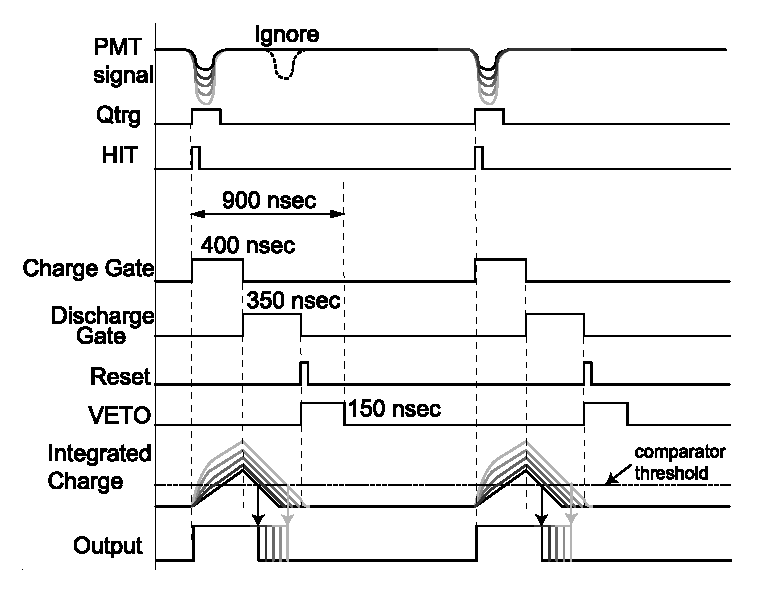
\includegraphics[width=12cm]{Figures/SK/QTCt}
%	\caption[Timing chart for QTC operation]{\label{SK_QTCt} Timing chart for QTC operation~\cite{2009Nishino}.}
%\end{figure}





\newpage



%
%	Simulation
%

\section{Simulation}\label{Section_Simula}
\Headerfooter{Simulation}





\subsection{Atmospheric neutrino flux}
\vs\hs
Many hadrons like pions and kaons are generated by reactions between a cosmic ray and a nucleus in the atmosphere.
The generated hadron decays into a muon and a neutrino, and the muon decays into an electron and two neutrinos.
The generated neutrinos in the atmosphere are called ``atmospheric neutrinos''.
Figure~\ref{Simula_AtmNeu} shows the schematic view of atmospheric neutrino production.

\begin{figure}[h]
	\centering
	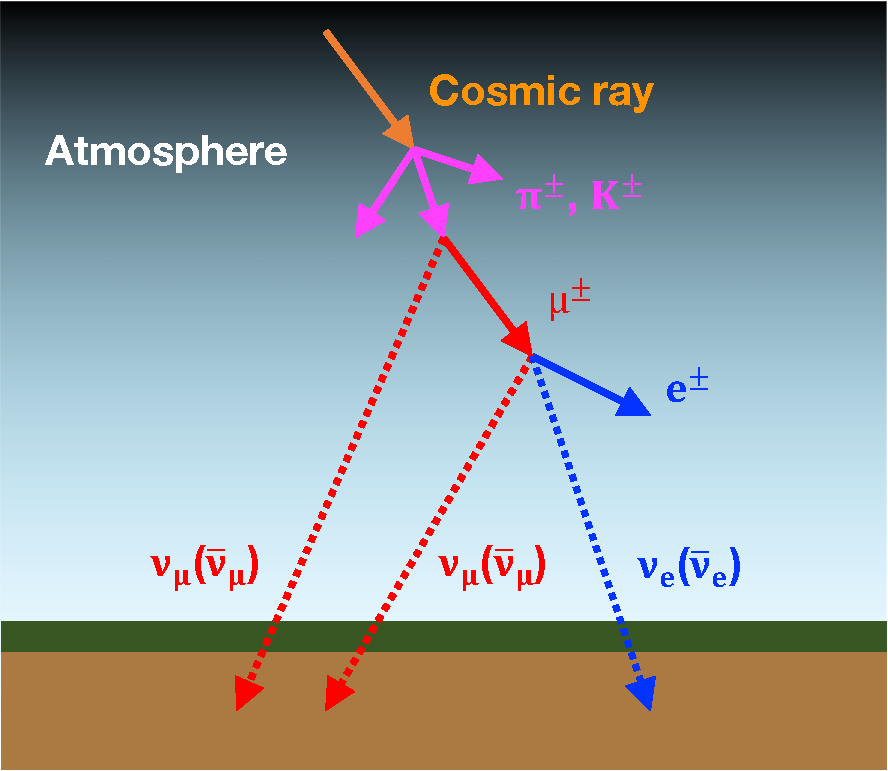
\includegraphics[width=6cm]{Figures/Simulation/AtmNeu}
	\caption[Schematic view of atmospheric neutrino production]{
	Schematic view of atmospheric neutrino production.
	}\label{Simula_AtmNeu}
\end{figure}

\hs
The atmospheric neutrino flux at the SK detector is predicted using the HKKM11 model~\cite{2011Honda}.
Figure~\ref{Simula_AtmNeuFlux} shows the atmospheric neutrino flux predicted by the HKKM11 model for the Kamioka site~\cite{2011Honda,2016Richard}.
As shown in this figure, the predicted flux shows good agreement with the observation in SK.
Atmospheric neutrino/antineutrino ratio and atmospheric neutrino flux of $\nu_{\rm e}\,+\,\nu_{\mu}$ ($\bar{\nu}_{\rm e}\,+\,\bar{\nu}_{\mu}$), $\nu_{\rm e}$ ($\bar{\nu}_{\rm e}$), and $\nu_{\mu}$ ($\bar{\nu}_{\mu}$) predicted by the HKKM11 model for the Kamioka site are shown in Figure~\ref{Simula_Ratio}~\cite{2011Honda}.
In this measurement, systematic uncertainties of atmospheric neutrino flux and atmospheric neutrino/antineutrino ratio are considered (see Section~\ref{SYSTEM}).

\begin{figure}[p]
	\centering
	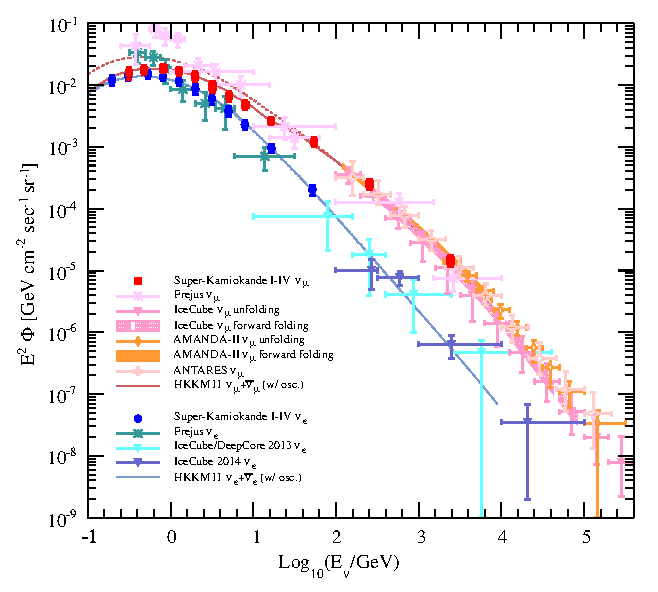
\includegraphics[width=8cm]{Figures/Simulation/AtmNeuFlux}
	\caption[Atmospheric neutrino flux predicted by the HKKM11 model for the Kamioka site]{
	Atmospheric neutrino flux predicted by the HKKM11 model for the Kamioka site~\cite{2011Honda,2016Richard}.
	Data plots are taken from the following experiments: Super-Kamiokande I-IV~\cite{2016Richard}, Frejus~\cite{1995Daum}, IceCube~\cite{2011Abbasi,2011Abbasi_02,2013Aartsen,2015Aartsen}, AMANDA-II~\cite{2009Abbasi,2010Abbasi}, and ANTARES~\cite{2013Adrian}.
	}\label{Simula_AtmNeuFlux}
\end{figure}

\begin{figure}[p]
	\centering
	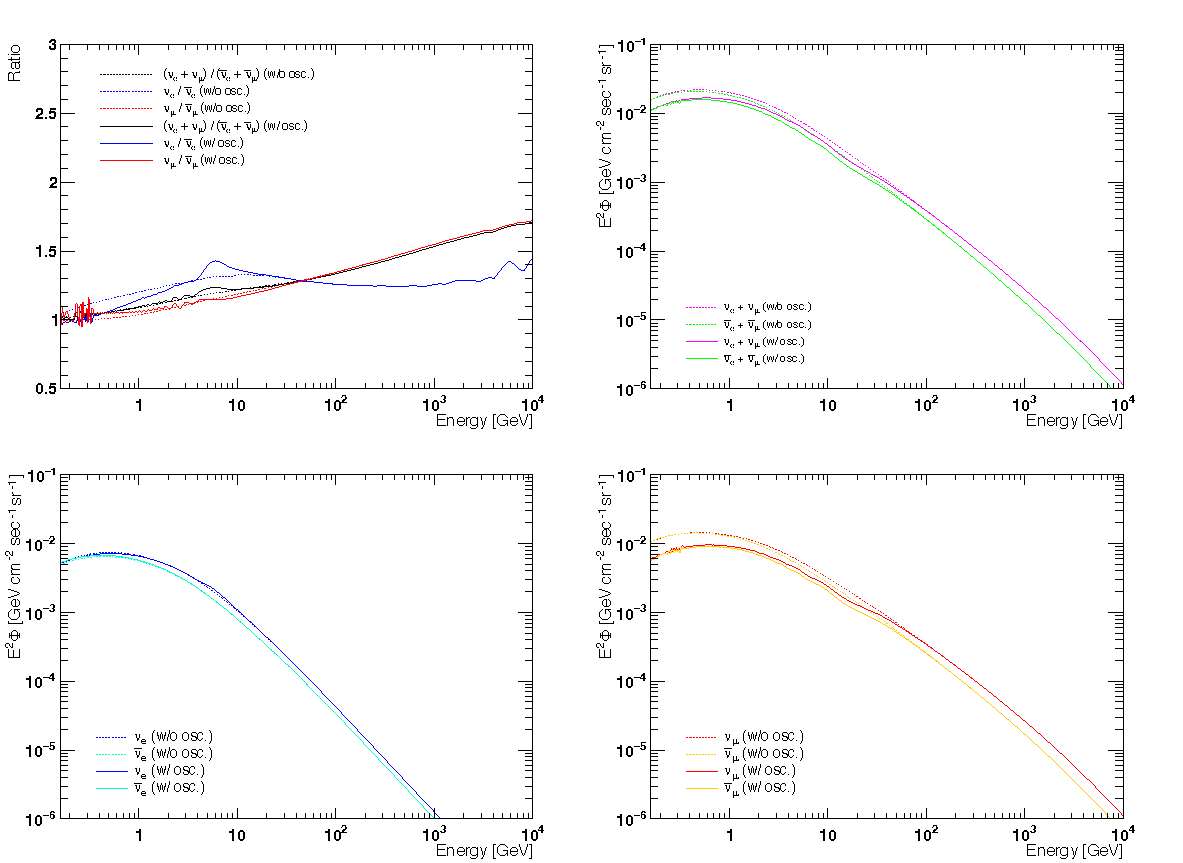
\includegraphics[width=16cm]{Figures/Simulation/Ratio}
	\caption[Atmospheric neutrino/antineutrino ratio and atmospheric neutrino flux of $\nu_{\rm e}\,+\,\nu_{\mu}$ ($\bar{\nu}_{\rm e}\,+\,\bar{\nu}_{\mu}$), $\nu_{\rm e}$ ($\bar{\nu}_{\rm e}$), and $\nu_{\mu}$ ($\bar{\nu}_{\mu}$) predicted by the HKKM11 model for the Kamioka site]{
	Atmospheric neutrino/antineutrino ratio (top left) and atmospheric neutrino flux of $\nu_{\rm e}\,+\,\nu_{\mu}$ ($\bar{\nu}_{\rm e}\,+\,\bar{\nu}_{\mu}$) (top right), $\nu_{\rm e}$ ($\bar{\nu}_{\rm e}$) (bottom left), and $\nu_{\mu}$ ($\bar{\nu}_{\mu}$) (bottom right) predicted by the HKKM11 model for the Kamioka site~\cite{2011Honda}.
	}\label{Simula_Ratio}
\end{figure}





\subsection{Neutirno interaction}\label{Subsec_neutrino_int}
\vs\hs
Neutrino interactions are simulated using NEUT~\cite{2021Hayato} (version 5.4.0.1).
Figure~\ref{CC_XS_numu} and Figure~\ref{CC_XS_nue} show the cross sections of charged-current interactions to nucleon used in NEUT (version 5.4.0.1).

\begin{figure}[tbp]
	\centering
	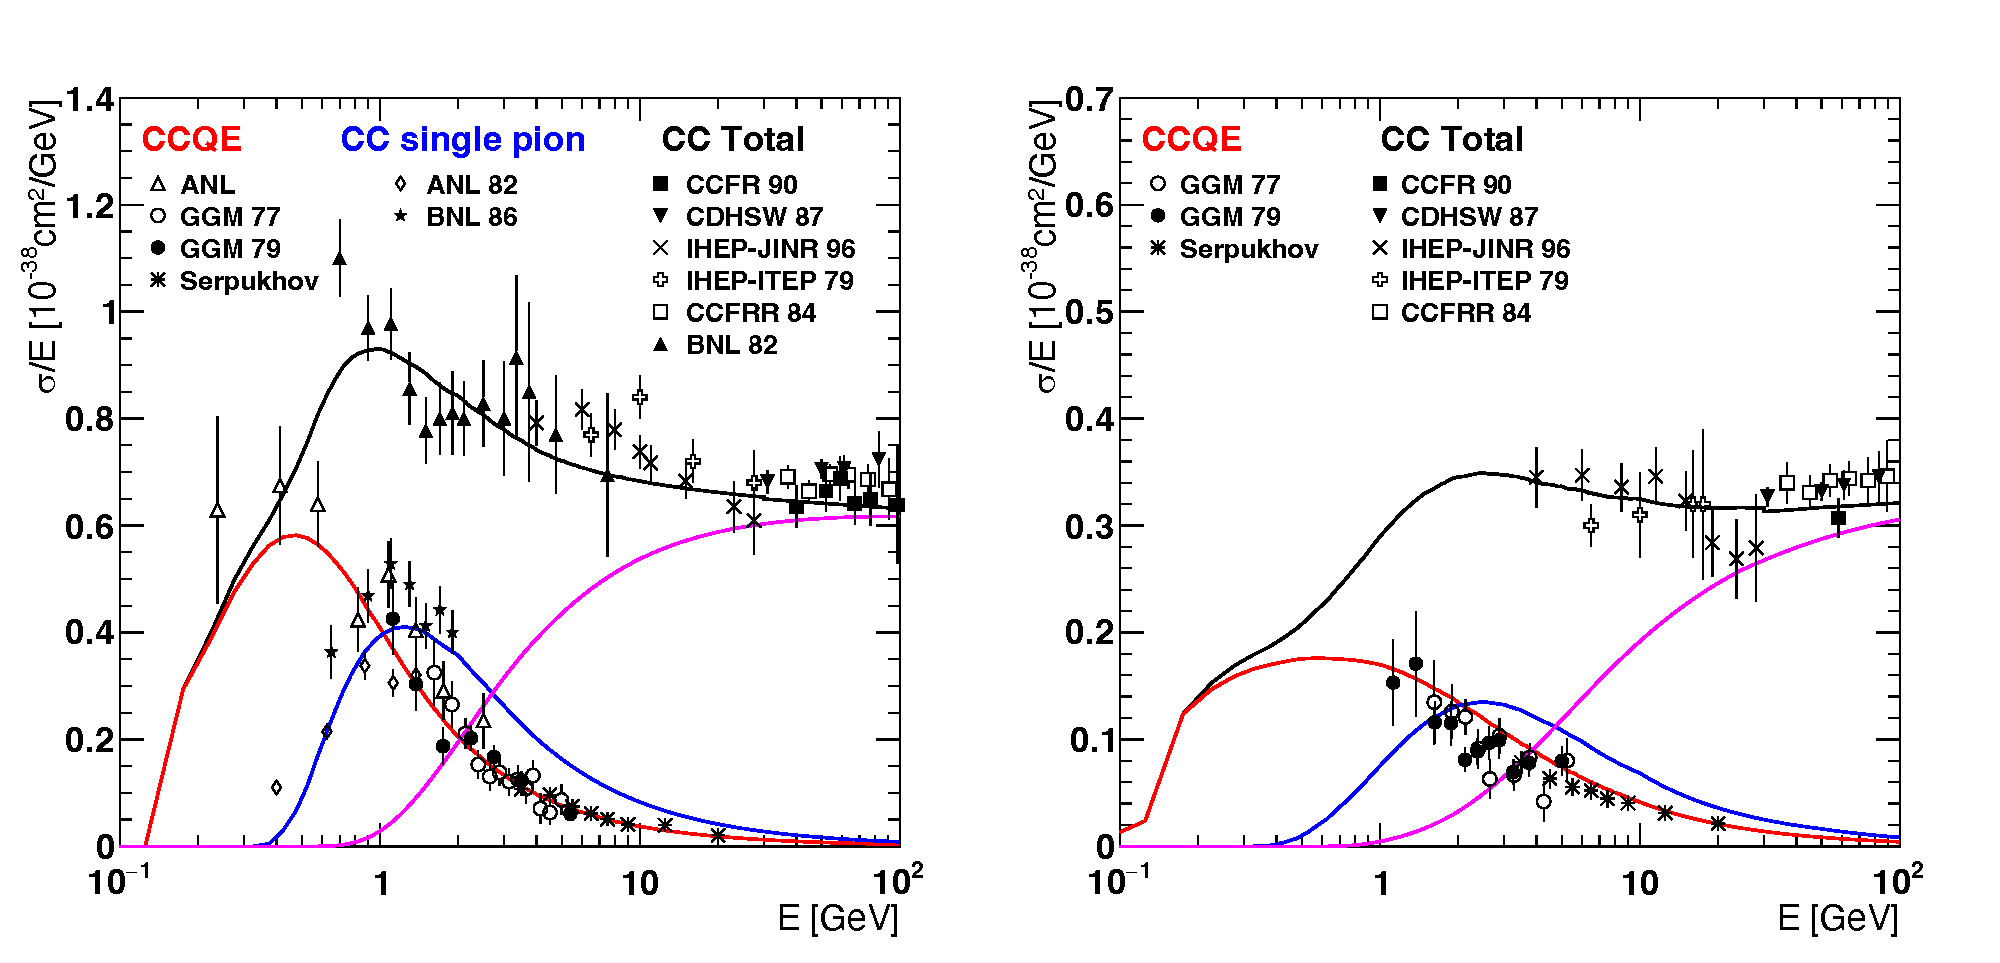
\includegraphics[width=16cm]{Figures/Simulation/CC_XS_numu}
	\caption[Cross sections of charged-current interactions to nucleon for $\nu_{\mu}$ and $\bar{\nu}_{\mu}$ used in NEUT (version 5.4.0.1)]{
	Cross sections of charged-current (CC) interactions to nucleon for $\nu_{\mu}$ (left) and $\bar{\nu}_{\mu}$ (right) used in NEUT (version 5.4.0.1).
	These figures are based on Figure~2 in Ref.~\cite{2020Koshio}.
	Red, blue, and magenta lines show the cross section of CC quasielastic (CCQE) scattering, CC single pion production, and CC deep inelastic scattering, respectively.
	Black line shows the CC total cross section.
	Data plots are taken from the following experiments:
	ANL~\cite{1977Barish}, GGM~77~\cite{1977Bonetti}, GGM~79 (left)~\cite{1979Ciampolillo}, GGM~79 (right)~\cite{1979Armenise}, Serpukhov~\cite{1985Belikov},
	ANL~82~\cite{1982Radecky}, BNL~86~\cite{1986Kitagaki},
	CCFR~90~\cite{1990Auchincloss}, CDHSW~87~\cite{1987Berge}, IHEP-JINR~96~\cite{1996Anikeev}, IHEP-ITEP~79~\cite{1979Mukhin}, CCFRR~84~\cite{1984MacFarlane}, and BNL~82~\cite{1982Baker}.
	}\label{CC_XS_numu}
\end{figure}

\begin{figure}[tbp]
	\centering
	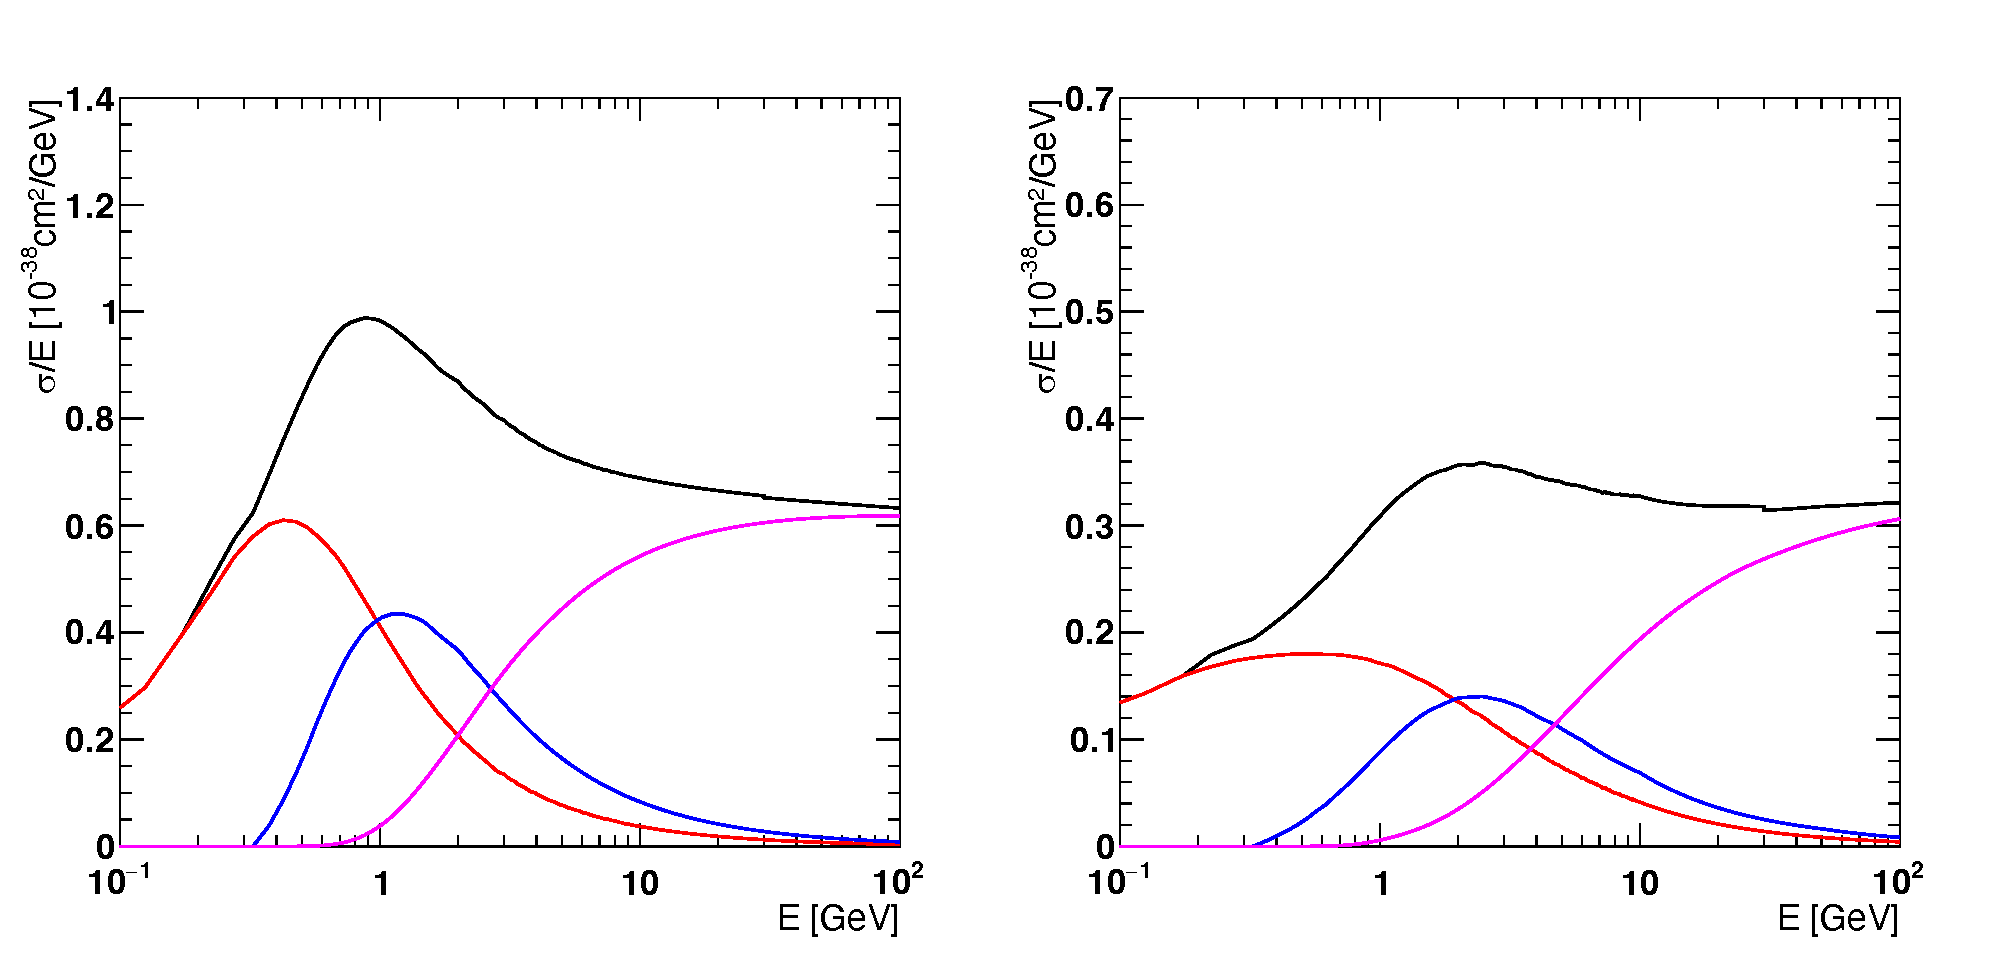
\includegraphics[width=16cm]{Figures/Simulation/CC_XS_nue}
	\caption[Cross sections of charged-current interactions to nucleon for $\nu_{\rm e}$ and $\bar{\nu}_{\rm e}$ used in NEUT (version 5.4.0.1)]{
	Cross sections of charged-current (CC) interactions to nucleon for $\nu_{\rm e}$ (left) and $\bar{\nu}_{\rm e}$ (right) used in NEUT (version 5.4.0.1).
	Red, blue, and magenta lines show the cross section of CC quasielastic (CCQE) scattering, CC single pion production, and CC deep inelastic scattering, respectively.
	Black line shows the CC total cross section.
	}\label{CC_XS_nue}
\end{figure}

\hs
Figure~\ref{NCQE} shows the schematic view of neutrino-oxygen NCQE scattering.
The NCQE cross section on oxygen is based on the model using the oxygen spectral function~\cite{2005Benhar,2012Ankowski} with the BBBA05 vector form factor~\cite{2006Bradford} and the dipole axial form factor~\cite{2006Bradford}.

\begin{figure}[tbp]
	\centering
	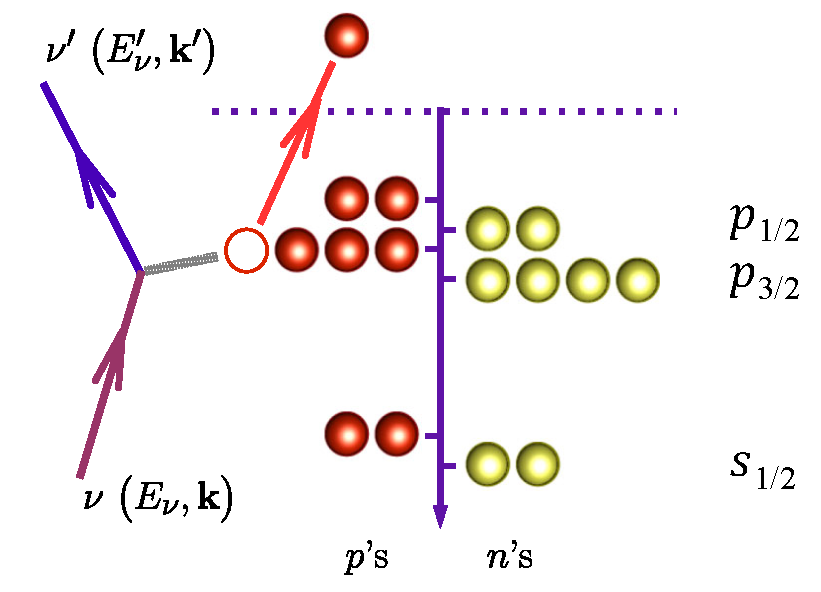
\includegraphics[width=8cm]{Figures/Simulation/NCQE}
	\caption[Schematic view of neutrino-oxygen NCQE scattering]{
	Schematic view of neutrino-oxygen NCQE scattering~\cite{2012Ankowski}.
	Dashed line represents the nucleon emission threshold.
	According to the shell model, protons and neutrons in the $^{16}{\rm O}$ nucleus occupy three states ($p_{1/2}$, $p_{3/2}$, and $s_{1/2}$).
	The removal energy of $p_{1/2}$ state, $p_{3/2}$ state, and $s_{1/2}$ state for protons is 12.1~MeV, 18.4~MeV, and $\sim$42~MeV, respectively.
	The removal energy for neutrons is 3.54~MeV larger than that for protons.
	}\label{NCQE}
\end{figure}

\hs
According to Ref.~\cite{2012Ankowski}, NCQE cross section is defined as
\begin{eqnarray}
	{d^{2}\sigma_{\nu A} \over d\Omega dE^{\prime}_{\nu}}=\sum_{N={\rm p},{\rm n}} \int d^{3}pdEP_{N}(\bm{p}, E){M \over E_{N}}{d^{2}\sigma_{\nu N} \over d\Omega dE^{\prime}_{\nu}},
\end{eqnarray}
where $M$ is the nucleon mass and $E_{N} = \sqrt{M^{2} + \bm{p}^{2}}$.
$P_{N}(\bm{p}, E)$ is the spectral function, that is, the probability of removing a nucleon of momentum $\bm{p}$ from the target leaving the residual nucleus with energy $E+E_{0}-M$, $E_{0}$ being the target ground state energy.
$d^{2}\sigma_{\nu N}/d\Omega dE^{\prime}_{\nu}$ is the neutrino-nucleon cross section.
In the nuclear shell model, the spectral function $P_{N}(\bm{p}, E)$ can be written in the form
\begin{eqnarray}
	P_{N}(\bm{p}, E)=\sum_{\alpha\in\{F\}} n_{\alpha}|\phi_{\alpha}(\bm{p})|^{2}f_{\alpha}(E-E_{\alpha}),
\end{eqnarray}
where $n_{\alpha}$ ($\leq 1$) is the occupation probability of the $\alpha$th state, $\phi_{\alpha}(\bm{p})$ is the momentum-space wave function associated with the $\alpha$th state, $f_{\alpha}(E-E_{\alpha})$ is the (unit-normalized) function describing the energy width of the $\alpha$th state, $-E_{\alpha}$ ($E_{\alpha}>0$) being the binding energy of the $\alpha$th state, and the sum is extended to all occupied states belonging to the Fermi sea $\{F\}$.
The neutrino-nucleon cross section $d^{2}\sigma_{\nu N}/d\Omega dE^{\prime}_{\nu}$ can be written in the form
\begin{eqnarray}
	{d^{2}\sigma_{\nu N} \over d\Omega dE^{\prime}_{\nu}}={G_{F}^{2} \over 8\pi^{2}}{E^{\prime}_{\nu} \over E_{\nu}}{L_{\mu\nu}W^{\mu\nu} \over ME^{\prime}_{N}}\delta(\tilde{\omega}+E_{N}-E^{\prime}_{N}),
\end{eqnarray}
where $G_{F}$ is the Fermi coupling constant and $E^{\prime}_{N} = \sqrt{M^{2} + \bm{p}^{\prime 2}}$.
The leptonic tensor $L_{\mu\nu}$ and the hadronic tensor $W^{\mu\nu}$ are given by
\begin{eqnarray}
	L_{\mu\nu}&=&2(k^{\prime}_{\mu}k_{\nu} + k^{\prime}_{\nu}k_{\mu} - g_{\mu\nu}k \cdot k^{\prime} - i\varepsilon_{\mu\nu\alpha\beta}k^{\alpha}k^{\prime\beta}), \\
	W^{\mu\nu}&=&-g^{\mu\nu}M^{2}W_{1} + \tilde{p}^{\mu}\tilde{p}^{\nu}W_{2} + i\varepsilon^{\mu\nu\alpha\beta}\tilde{p}_{\alpha}\tilde{q}_{\beta}W_{3} + \tilde{q}^{\mu}\tilde{q}^{\nu}W_{4} + (\tilde{p}^{\mu}\tilde{q}^{\nu} + \tilde{p}^{\nu}\tilde{q}^{\mu})W_{5},
\end{eqnarray}
where $\tilde{p}=(E_{N}, \bm{p})$ and $\tilde{q}=(\tilde{\omega}, \bm{k} - \bm{k}^{\prime})$.
The structure functions $W_{i}$ ($i=1,2,3,4,5$) can be written as
\begin{eqnarray}
	W_{1}&=&\tau(\mathcal{F}^{N}_{1} + \mathcal{F}^{N}_{2})^{2} + (1 + \tau)\mathcal{F}^{2}_{A}, \nonumber \\
	W_{2}&=&(\mathcal{F}^{N}_{1})^{2} + \tau(\mathcal{F}^{N}_{2})^{2} + \mathcal{F}^{2}_{A}, \nonumber \\
	W_{3}&=&(\mathcal{F}^{N}_{1} + \mathcal{F}^{N}_{2})\mathcal{F}_{A}, \nonumber \\
	W_{4}&=&{1 \over 4}[(\mathcal{F}^{N}_{1})^{2} + \tau(\mathcal{F}^{N}_{2})^{2} - (\mathcal{F}^{N}_{1} + \mathcal{F}^{N}_{2})^{2} - 4\mathcal{F}_{P}(\mathcal{F}_{A} - \tau\mathcal{F}_{P})], \nonumber \\
	W_{5}&=&{1 \over 2}W_{2},
\end{eqnarray}
where $\tau = -\tilde{q}^{2}/(4M^{2})$.
The nucleon form factors \{$\mathcal{F}^{N}_{i}$ ($i=1,2$), $\mathcal{F}_{A}$, $\mathcal{F}_{P}$\} can be written as
\begin{eqnarray}
	\mathcal{F}^{N}_{1}&=&\pm{1 \over 2}(F^{{\rm p}}_{1} - F^{{\rm n}}_{1}) - 2\sin^{2}\theta_{W}F^{N}_{1}, \nonumber \\
	\mathcal{F}^{N}_{2}&=&\pm{1 \over 2}(F^{{\rm p}}_{2} - F^{{\rm n}}_{2}) - 2\sin^{2}\theta_{W}F^{N}_{2}, \nonumber \\
	\mathcal{F}_{A}    &=&{1 \over 2}{\Delta s \pm g_{A} \over (1 - \tilde{q}^{2}/M_{A}^{2})^{2}}, \nonumber \\
	\mathcal{F}_{P}    &=&{2M^{2}\mathcal{F}_{A} \over m_{\pi}^{2} - \tilde{q}^{2}},
\end{eqnarray}
where the upper (lower) sign corresponds to proton (neutron) form factors, $\theta_{W}$ is the weak mixing angle, $\Delta s$ ($=-0.08$) is the strange quark contribution, $g_{A}=-1.2673$, $M_{A}$ is the axial mass, and $m_{\pi}$ is the pion mass.
The form factors $F^{N}_{1}$ and $F^{N}_{2}$ can be expressed as
\begin{eqnarray}
	F^{N}_{1}&=&{G^{N}_{E} + \tau G^{N}_{M} \over 1 + \tau}, \nonumber \\
	F^{N}_{2}&=&{G^{N}_{M} - G^{N}_{E} \over 1 + \tau},
\end{eqnarray}
where $G^{N}_{E}$ is the electric form factors and $G^{N}_{M}$ is the magnetic form factors.
Figure~\ref{Simula_NCQECroSec} shows the NCQE cross section on nucleon and on oxygen nucleus as a function of neutrino energy.
Figure~\ref{BBBA05} shows the ratio of the BBBA05 vector form factors to $G_{d}$ (the dipole axial form factor).\\
\hs
The state of the residual nucleus after primary interaction (see Figure~\ref{Introd_NCQE_PriSec}) is selected based on the probabilities computed in Ref.~\cite{2012Ankowski}.
There are four states, $(p_{1/2})^{-1}$, $(p_{3/2})^{-1}$, $(s_{1/2})^{-1}$, and \textit{others}, where $($state$)^{-1}$ shows the state of the nucleus after a nucleon initially occupying the state ($p_{1/2}$, $p_{3/2}$, or $s_{1/2}$) is removed.
The production probability of each state is 0.1580, 0.3515, 0.1055, and 0.3850, respectively.
The production probabilities of $(p_{1/2})^{-1}$ state, $(p_{3/2})^{-1}$ state, and $(s_{1/2})^{-1}$ state are obtained by multiplying the spectroscopic strength by the probability that a nucleon in the state is knocked out.
Spectroscopic strengths of the $^{16}{\rm O}$ hole states and probabilities that a nucleon in the state is knocked out are summarized in Table~\ref{Spec}.
The production probability of \textit{others} state is equal to 1~$-$~0.1580~$-$~0.3515~$-$~0.1055.

\begin{figure}[H]
	\centering
	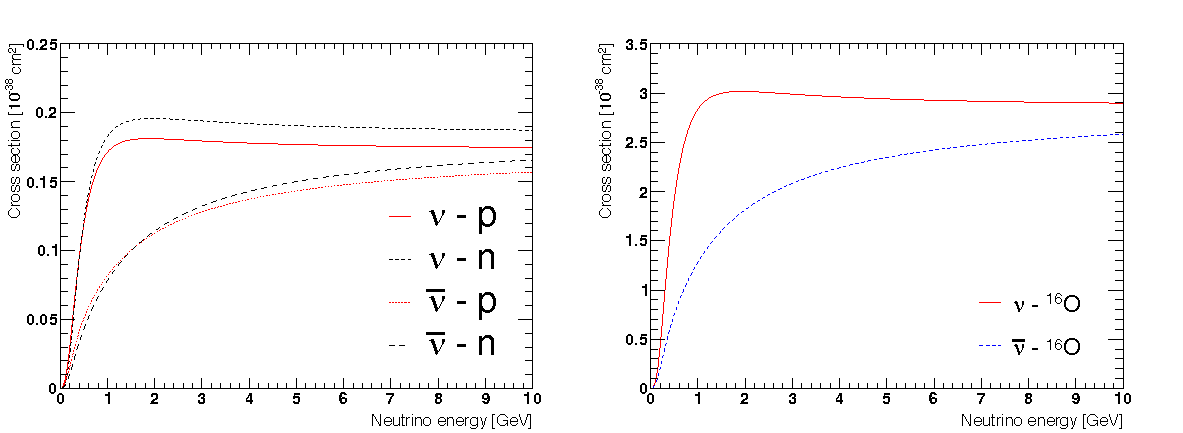
\includegraphics[width=16cm]{Figures/Simulation/NCQECroSec}
	\caption[NCQE cross section on nucleon and on oxygen nucleus as a function of neutrino energy]{
	NCQE cross section on nucleon (left) and on oxygen nucleus (right) as a function of neutrino energy~\cite{2012Ankowski}.
	}\label{Simula_NCQECroSec}
\end{figure}

\begin{figure}[H]
	\centering
	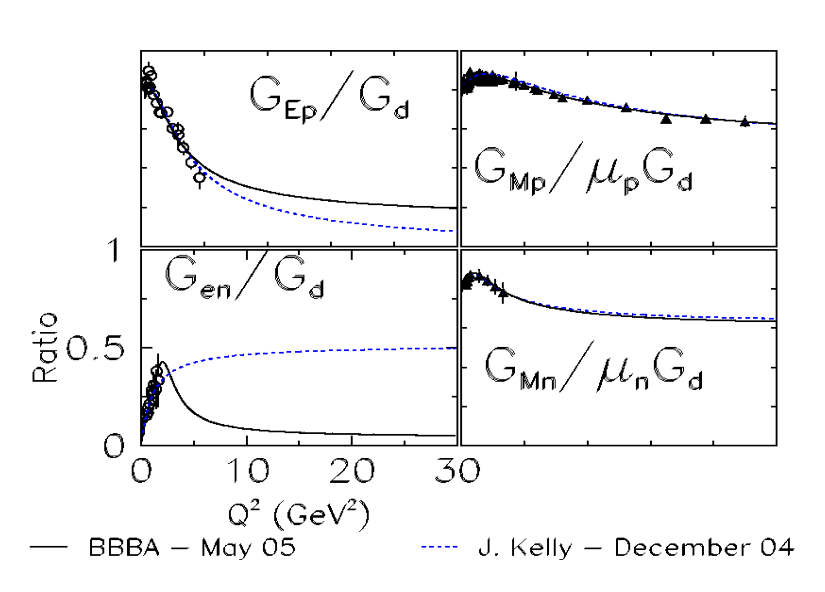
\includegraphics[width=10cm]{Figures/Simulation/BBBA05}
	\caption[The ratio of the BBBA05 vector form factors to $G_{d}$]{
	The ratio of the BBBA05 vector form factors to $G_{d}$ (the dipole axial form factor) (shown in the solid brack line)\cite{2006Bradford}.
	The dashed blue line shows the ratio of the Kelly form factors to $G_{d}$.
	}\label{BBBA05}
\end{figure}

\begin{table}[H]
	\centering
	\caption[Spectroscopic strengths of the $^{16}{\rm O}$ hole states and probabilities that a nucleon in the state is knocked out]{
	Spectroscopic strengths of the $^{16}{\rm O}$ hole states ($S_{\alpha}$) and probabilities that a nucleon in the state is knocked out ($P_{\alpha}$)~\cite{2012Ankowski}.
	}\label{Spec}
	\vs
	\begin{tabular}{lrrr} \hline \hline
		$\alpha$     & $p_{1/2}$ & $p_{3/2}$ & $s_{1/2}$ \\ \hline
		$S_{\alpha}$ & 0.632     & 0.703     & 0.422     \\
		$P_{\alpha}$ & 2$/$8     & 4$/$8     & 2$/$8     \\ \hline \hline
	\end{tabular}
\end{table}

\hs
$(p_{1/2})^{-1}$ state is the ground state of $^{15}{\rm O}$ or $^{15}{\rm N}$, thus no gamma-ray is emitted.
Mainly 6.18~MeV or 6.32~MeV gamma-rays are emitted from $(p_{3/2})^{-1}$ state of $^{15}{\rm O}$ or $^{15}{\rm N}$, respectively~\cite{1994Leuschner,1991Ajzenberg}.
De-excitation modes of $(p_{3/2})^{-1}$ state implemented in NEUT are summarized in Table~\ref{deex_p3_2_O} and Table~\ref{deex_p3_2_N}.
In the case of $(s_{1/2})^{-1}$ state, nucleons and gamma-rays are emitted because the excitation energy is high.
The de-excitation mode is selected based on the $^{16}{\rm O}({\rm p}, 2{\rm p})$ experiment~\cite{2006Kobayashi}.
De-excitation modes of $(s_{1/2})^{-1}$ state implemented in NEUT are summarized in Table~\ref{deex_s1_2_O} and Table~\ref{deex_s1_2_N}.
In the case that the residual nuclei are $^{14}{\rm N}\,+\,{\rm p}$, kinetic energy of generated proton ($E_{{\rm p}}$) is calculated by
\begin{eqnarray}\label{Ep_14Np}
	E_{{\rm p}} = {\rm max}\bigg[0,\,(39.5 \times \eta + 10.65 - E_{l} - E_{^{14}{\rm N}\,+\,{\rm p}}) \times {m_{^{14}{\rm N}} + E_{l} \over m_{{\rm p}} + m_{^{14}{\rm N}} + E_{l}}\bigg],
\end{eqnarray}
where $\eta$ is a random number uniformly distributed in the range from 0 to 1, $E_{l}$ is the energy level, $E_{^{14}{\rm N}\,+\,{\rm p}}$ ($=7.30~{\rm MeV}$) is the energy threshold of two-body decay from $^{15}{\rm O}$ to $^{14}{\rm N}\,+\,{\rm p}$, $m_{^{14}{\rm N}}$ ($=13043.78~{\rm MeV}$) is the mass of $^{14}{\rm N}$ ground state, and $m_{{\rm p}}$ ($=938.27~{\rm MeV}$) is the proton mass.
In the case that the residual nuclei are $^{14}{\rm O}\,+\,{\rm n}$, kinetic energy of generated neutron ($E_{{\rm n}}$) is calculated by
\begin{eqnarray}\label{En_14On}
	E_{{\rm n}} = {\rm max}\bigg[0,\,(39.5 \times \eta + 10.65 - E_{l} - E_{^{14}{\rm O}\,+\,{\rm n}}) \times {m_{^{14}{\rm O}} + E_{l} \over m_{{\rm n}} + m_{^{14}{\rm O}} + E_{l}}\bigg],
\end{eqnarray}
where $E_{^{14}{\rm O}\,+\,{\rm n}}$ ($=13.22~{\rm MeV}$) is the energy threshold of two-body decay from $^{15}{\rm O}$ to $^{14}{\rm O}\,+\,{\rm n}$, $m_{^{14}{\rm O}}$ ($=13048.92~{\rm MeV}$) is the mass of $^{14}{\rm O}$ ground state, and $m_{{\rm n}}$ ($=939.56~{\rm MeV}$) is the neutron mass.
In the case that the residual nuclei are $^{14}{\rm N}\,+\,{\rm n}$, $E_{{\rm n}}$ is calculated by
\begin{eqnarray}\label{En_14Nn}
	E_{{\rm n}} = {\rm max}\bigg[0,\,(39.5 \times \eta + 10.65 - E_{l} - E_{^{14}{\rm N}\,+\,{\rm n}}) \times {m_{^{14}{\rm N}} + E_{l} \over m_{{\rm n}} + m_{^{14}{\rm N}} + E_{l}}\bigg],
\end{eqnarray}
where $E_{^{14}{\rm N}\,+\,{\rm n}}$ ($=10.83~{\rm MeV}$) is the energy threshold of two-body decay from $^{15}{\rm N}$ to $^{14}{\rm N}\,+\,{\rm n}$.
In the case that the residual nuclei are $^{14}{\rm C}\,+\,{\rm p}$, $E_{{\rm p}}$ is calculated by
\begin{eqnarray}\label{Ep_14Cp}
	E_{{\rm p}} = {\rm max}\bigg[0,\,(39.5 \times \eta + 10.65 - E_{l} - E_{^{14}{\rm C}\,+\,{\rm p}}) \times {m_{^{14}{\rm C}} + E_{l} \over m_{{\rm p}} + m_{^{14}{\rm C}} + E_{l}}\bigg],
\end{eqnarray}
where $E_{^{14}{\rm C}\,+\,{\rm p}}$ ($=10.21~{\rm MeV}$) is the energy threshold of two-body decay from $^{15}{\rm N}$ to $^{14}{\rm C}\,+\,{\rm p}$ and $m_{^{14}{\rm C}}$ ($=13043.94~{\rm MeV}$) is the mass of $^{14}{\rm C}$ ground state.
The \textit{others} state includes all other possibilities that are not in $(p_{1/2})^{-1}$, $(p_{3/2})^{-1}$, and $(s_{1/2})^{-1}$ states, and there are no data nor theoretical predictions covered by this state.
In our simulation, the \textit{others} state is set to be integrated into $(s_{1/2})^{-1}$ state by default.\\
\hs
Other distributions related to this section are summarized in Appendix~\ref{App_Simula}.

\begin{table}[H]
	\centering
	\caption[De-excitation modes of $(p_{3/2})^{-1}$ state for $^{15}{\rm O}$ implemented in NEUT]{
	De-excitation modes of $(p_{3/2})^{-1}$ state for $^{15}{\rm O}$ implemented in NEUT.
	$E_{\gamma}$ and $E_{{\rm p}}$ show the (kinetic) energy of generated gamma-ray and generated proton, respectively.
	Probabilities that the mode is selected in NEUT are summarized in the rightmost column.
	Please also check Ref.~\cite{1994Leuschner,1991Ajzenberg}.
	}\label{deex_p3_2_O}
	\vs
	\begin{tabular}{ccccc} \hline \hline
		Residual nuclei            & Energy level  & $E_{\gamma}$  & $E_{{\rm p}}$ & Probability \\
		                           & $({\rm MeV})$ & $({\rm MeV})$ & $({\rm MeV})$ &             \\ \hline
		$^{15}{\rm O}$             & 6.18          & 6.18          & -             & 86.86\%     \\
		$^{14}{\rm N}\,+\,{\rm p}$ & 9.61          & -             & 0.5           & 4.92\%      \\
		$^{14}{\rm N}\,+\,{\rm p}$ & 10.48         & -             & 0.5           & 8.22\%      \\ \hline \hline
	\end{tabular}
\end{table}

\begin{table}[H]
	\centering
	\caption[De-excitation modes of $(p_{3/2})^{-1}$ state for $^{15}{\rm N}$ implemented in NEUT]{
	De-excitation modes of $(p_{3/2})^{-1}$ state for $^{15}{\rm N}$ implemented in NEUT.
	$E_{\gamma}$ and $E_{{\rm p}}$ show the (kinetic) energy of generated gamma-rays and generated proton, respectively.
	Probabilities that the mode is selected in NEUT are summarized in the rightmost column.
	Please also check Ref.~\cite{1994Leuschner,1991Ajzenberg}.
	}\label{deex_p3_2_N}
	\vs
	\begin{tabular}{ccccc} \hline \hline
		Residual nuclei            & Energy level  & $E_{\gamma}$    & $E_{{\rm p}}$ & Probability \\
		                           & $({\rm MeV})$ & $({\rm MeV})$   & $({\rm MeV})$ &             \\ \hline
		$^{15}{\rm N}$             & 6.32          & 6.32            & -             & 86.86\%     \\
		$^{15}{\rm N}$             & 9.93          & 9.93            & -             & 3.82\%      \\
		$^{15}{\rm N}$             & 9.93          & 5.30$\,+\,$4.64 & -             & 0.76\%      \\
		$^{15}{\rm N}$             & 9.93          & 6.32$\,+\,$3.61 & -             & 0.24\%      \\
		$^{15}{\rm N}$             & 9.93          & 7.30$\,+\,$2.63 & -             & 0.10\%      \\
		$^{14}{\rm C}\,+\,{\rm p}$ & 10.70         & -               & 0.5           & 8.22\%      \\ \hline \hline
	\end{tabular}
\end{table}

\begin{table}[h]
	\centering
	\caption[De-excitation modes of $(s_{1/2})^{-1}$ state for $^{15}{\rm O}$ implemented in NEUT]{
	De-excitation modes of $(s_{1/2})^{-1}$ state for $^{15}{\rm O}$ implemented in NEUT.
	$E_{\gamma}$, $E_{{\rm n}}$, and $E_{{\rm p}}$ show the (kinetic) energy of generated gamma-ray, generated neutron, and generated proton, respectively.
	Probabilities that the mode is selected in NEUT are summarized in the rightmost column.
	The last two rows consider the three-body decay of $^{15}{\rm O}$.
	Please also check Ref.~\cite{2006Kobayashi}.
	}\label{deex_s1_2_O}
	\vs
	\begin{tabular}{cccccc} \hline \hline
		Residual nuclei            & Energy level  & $E_{\gamma}$  & $E_{{\rm n}}$            & $E_{{\rm p}}$            & Probability \\
		                           & $({\rm MeV})$ & $({\rm MeV})$ & $({\rm MeV})$            & $({\rm MeV})$            &             \\ \hline
		$^{13}{\rm N}\,+\,{\rm d}$ & 3.09          & 3.09          & -                        & -                        & 3.00\%      \\
		$^{13}{\rm N}\,+\,{\rm d}$ & 3.68          & 3.68          & -                        & -                        & 4.17\%      \\
		$^{13}{\rm N}\,+\,{\rm d}$ & 3.85          & 3.68          & -                        & -                        & 1.67\%      \\
		$^{13}{\rm N}\,+\,{\rm d}$ & 3.85          & 3.85          & -                        & -                        & 2.88\%      \\
		$^{12}{\rm N}\,+\,{\rm t}$ & 4.44          & 4.44          & -                        & -                        & 5.80\%      \\
		$^{14}{\rm N}\,+\,{\rm p}$ & g.s.          & -             & -                        & Equation~(\ref{Ep_14Np}) & 6.74\%      \\
		$^{14}{\rm N}\,+\,{\rm p}$ & 4.92          & 4.92          & -                        & Equation~(\ref{Ep_14Np}) & 5.04\%      \\
		$^{14}{\rm N}\,+\,{\rm p}$ & 5.69          & 3.38          & -                        & Equation~(\ref{Ep_14Np}) & 2.88\%      \\
		$^{14}{\rm N}\,+\,{\rm p}$ & 5.69          & 5.69          & -                        & Equation~(\ref{Ep_14Np}) & 1.62\%      \\
		$^{14}{\rm N}\,+\,{\rm p}$ & 5.83          & 5.11          & -                        & Equation~(\ref{Ep_14Np}) & 0.34\%      \\
		$^{14}{\rm N}\,+\,{\rm p}$ & 5.83          & 5.83          & -                        & Equation~(\ref{Ep_14Np}) & 0.12\%      \\
		$^{14}{\rm N}\,+\,{\rm p}$ & 6.45          & 5.11          & -                        & Equation~(\ref{Ep_14Np}) & 0.23\%      \\
		$^{14}{\rm N}\,+\,{\rm p}$ & 6.45          & 6.44          & -                        & Equation~(\ref{Ep_14Np}) & 1.96\%      \\
		$^{14}{\rm N}\,+\,{\rm p}$ & 7.03          & 7.03          & -                        & Equation~(\ref{Ep_14Np}) & 6.61\%      \\
		$^{14}{\rm O}\,+\,{\rm n}$ & g.s.          & -             & Equation~(\ref{En_14On}) & -                        & 1.15\%      \\
		$^{14}{\rm O}\,+\,{\rm n}$ & 6.73          & 6.73          & Equation~(\ref{En_14On}) & -                        & 0.41\%      \\
		$^{14}{\rm O}\,+\,{\rm n}$ & 7.34          & 6.09          & Equation~(\ref{En_14On}) & -                        & 2.79\%      \\
		$^{14}{\rm O}\,+\,{\rm n}$ & 7.34          & 6.73          & Equation~(\ref{En_14On}) & -                        & 1.96\%      \\
		$^{14}{\rm O}\,+\,{\rm n}$ & 7.34          & 7.34          & Equation~(\ref{En_14On}) & -                        & 0.95\%      \\
		-                          & -             & -             & -                        & 0--5                     & 31.90\%     \\
		-                          & -             & -             & 0--5                     & -                        & 17.78\%     \\ \hline \hline
	\end{tabular}
\end{table}

\begin{table}[h]
	\centering
	\caption[De-excitation modes of $(s_{1/2})^{-1}$ state for $^{15}{\rm N}$ implemented in NEUT]{
	De-excitation modes of $(s_{1/2})^{-1}$ state for $^{15}{\rm N}$ implemented in NEUT.
	$E_{\gamma}$, $E_{{\rm n}}$, and $E_{{\rm p}}$ show the (kinetic) energy of generated gamma-ray, generated neutron, and generated proton, respectively.
	Probabilities that the mode is selected in NEUT are summarized in the rightmost column.
	The last two rows consider the three-body decay of $^{15}{\rm N}$.
	Please also check Ref.~\cite{2006Kobayashi}.
	}\label{deex_s1_2_N}
	\vs
	\begin{tabular}{cccccc} \hline \hline
		Residual nuclei            & Energy level  & $E_{\gamma}$  & $E_{{\rm n}}$            & $E_{{\rm p}}$            & Probability \\
		                           & $({\rm MeV})$ & $({\rm MeV})$ & $({\rm MeV})$            & $({\rm MeV})$            &             \\ \hline
		$^{13}{\rm C}\,+\,{\rm d}$ & 3.09          & 3.09          & -                        & -                        & 3.00\%      \\
		$^{13}{\rm C}\,+\,{\rm d}$ & 3.68          & 3.68          & -                        & -                        & 4.17\%      \\
		$^{13}{\rm C}\,+\,{\rm d}$ & 3.85          & 3.68          & -                        & -                        & 1.67\%      \\
		$^{13}{\rm C}\,+\,{\rm d}$ & 3.85          & 3.85          & -                        & -                        & 2.88\%      \\
		$^{12}{\rm C}\,+\,{\rm t}$ & 4.44          & 4.44          & -                        & -                        & 5.80\%      \\
		$^{14}{\rm N}\,+\,{\rm n}$ & g.s.          & -             & Equation~(\ref{En_14Nn}) & -                        & 6.74\%      \\
		$^{14}{\rm N}\,+\,{\rm n}$ & 4.92          & 4.92          & Equation~(\ref{En_14Nn}) & -                        & 5.04\%      \\
		$^{14}{\rm N}\,+\,{\rm n}$ & 5.69          & 3.38          & Equation~(\ref{En_14Nn}) & -                        & 2.88\%      \\
		$^{14}{\rm N}\,+\,{\rm n}$ & 5.69          & 5.69          & Equation~(\ref{En_14Nn}) & -                        & 1.62\%      \\
		$^{14}{\rm N}\,+\,{\rm n}$ & 5.83          & 5.11          & Equation~(\ref{En_14Nn}) & -                        & 0.34\%      \\
		$^{14}{\rm N}\,+\,{\rm n}$ & 5.83          & 5.83          & Equation~(\ref{En_14Nn}) & -                        & 0.12\%      \\
		$^{14}{\rm N}\,+\,{\rm n}$ & 6.45          & 5.11          & Equation~(\ref{En_14Nn}) & -                        & 0.23\%      \\
		$^{14}{\rm N}\,+\,{\rm n}$ & 6.45          & 6.44          & Equation~(\ref{En_14Nn}) & -                        & 1.96\%      \\
		$^{14}{\rm N}\,+\,{\rm n}$ & 7.03          & 7.03          & Equation~(\ref{En_14Nn}) & -                        & 6.61\%      \\
		$^{14}{\rm C}\,+\,{\rm p}$ & g.s.          & -             & -                        & Equation~(\ref{Ep_14Cp}) & 1.15\%      \\
		$^{14}{\rm C}\,+\,{\rm p}$ & 6.73          & 6.73          & -                        & Equation~(\ref{Ep_14Cp}) & 0.41\%      \\
		$^{14}{\rm C}\,+\,{\rm p}$ & 7.34          & 6.09          & -                        & Equation~(\ref{Ep_14Cp}) & 2.79\%      \\
		$^{14}{\rm C}\,+\,{\rm p}$ & 7.34          & 6.73          & -                        & Equation~(\ref{Ep_14Cp}) & 1.96\%      \\
		$^{14}{\rm C}\,+\,{\rm p}$ & 7.34          & 7.34          & -                        & Equation~(\ref{Ep_14Cp}) & 0.95\%      \\
		-                          & -             & -             & 0--5                     & -                        & 31.90\%     \\
		-                          & -             & -             & -                        & 0--5                     & 17.78\%     \\ \hline \hline
	\end{tabular}
\end{table}





\clearpage
\subsection{Simulation for the IBD-like event}
\vs\hs
Spallation events, reactor neutrino events, and DSNB events are estimated by generating one positron and one neutron isotropically over the entire ID in MC.
Moreover, the positron energy is uniform.
The number of events is later normalized by using neutrino flux or positron (electron) energy spectrum.
Details for the normalization are summarized below.

\subsubsection{Spallation events}\label{Subsubsec_sim_spa}
\vs\hs
Spallation events are decays of radioactive isotopes produced by nuclear spallation of oxygen nuclei induced by energetic cosmic ray muons.
Figure~\ref{Simulation_Spallation_event} shows the schematic view of a spallation event.
Some radioactive isotopes emit one electron and one neutron, mimicing the IBD events.
Most of them can be ignored due to a short lifetime and a low yield, however, $^{9}{\rm Li}$ cannot be ignored because of a relatively long lifetime ($\sim$0.26~s) and a large yield ($1.9 \times 50.8\% \times 10^{-7} \mu^{-1}g^{-1}{\rm cm}^{2}$)~\cite{2007Battistoni}.
Therefore, the number of events is normalized by using the energy spectrum of electrons from $^{9}{\rm Li}$ decays and the measured $^{9}{\rm Li}$ rate at SK ($0.86\,\pm\,0.12 ({\rm stat.})\,\pm\,0.15 ({\rm syst.})\,{\rm kton}^{-1}{\rm day}^{-1}$)~\cite{2015Zhang}.
Figure~\ref{9Li_ene} shows the energy spectrum of electrons from $^{9}{\rm Li}$ decays modeled by the BESTIOLE code~\cite{2010ThomasPhD}.

\begin{figure}[H]
	\centering
	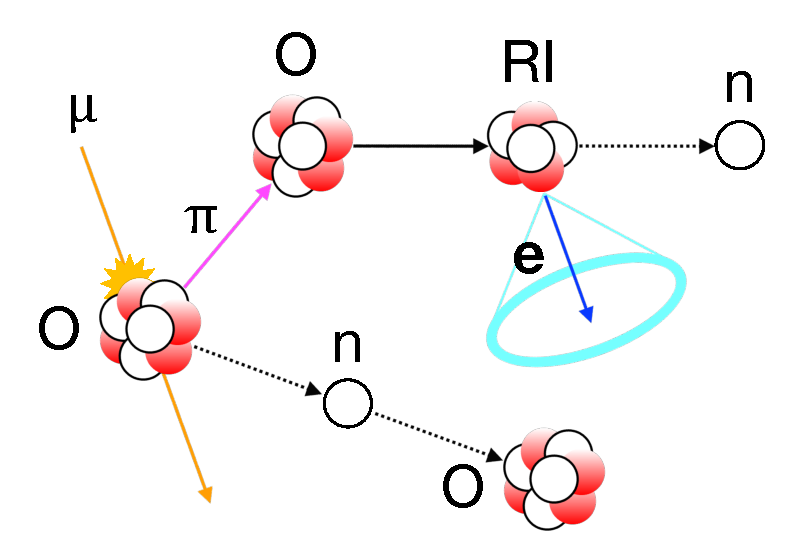
\includegraphics[width=6cm]{Figures/Simulation/Spallation_event}
	\caption[Schematic view of a spallation event]{
	Schematic view of a spallation event.
	RI stands for radioactive isotope.
	}\label{Simulation_Spallation_event}
\end{figure}

\begin{figure}[H]
	\centering
	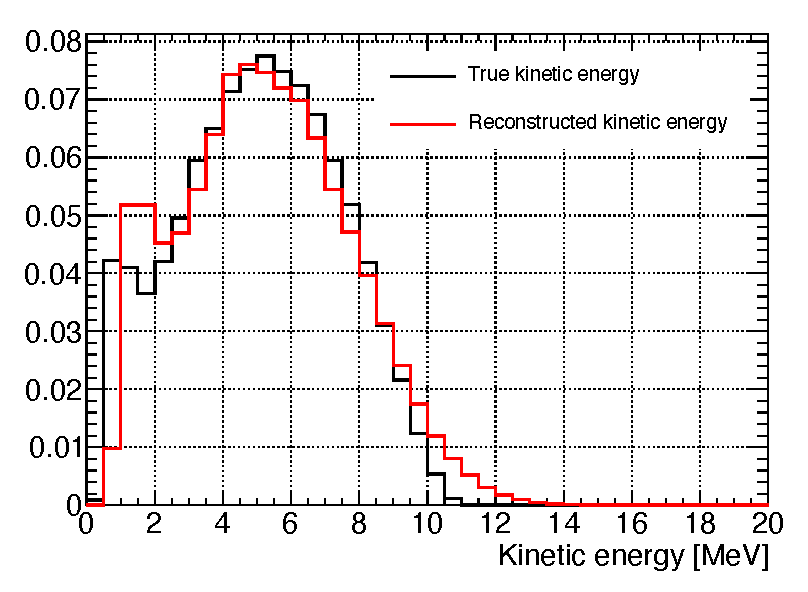
\includegraphics[width=8cm]{Figures/Simulation/9Li_ene}
	\caption[Energy spectrum of electrons from $^{9}{\rm Li}$ decays modeled by the BESTIOLE code]{
	Energy spectrum of electrons from $^{9}{\rm Li}$ decays modeled by the BESTIOLE code~\cite{2010ThomasPhD,2023HaradaPhD}.
	Red line shows the reconstructed energy spectrum.
	}\label{9Li_ene}
\end{figure}

\subsubsection{Reactor neutrino events}\label{Subsubsec_sim_reactor}
\vs\hs
While reactors are operating, many electron antineutrinos are generated via beta decays.
Reactor neutrino events are also the IBD events by electron antineutrinos from reactors.
The reactor neutrino flux is calculated using SKReact\footnote{If you would like to know how to use SKReact, please check the url (\url{https://github.com/Goldie643/SKReact}).}, which is a tool for calculating the electron antineutrino flux from reactors, considering the activity of each reactor near the SK.
Figure~\ref{Reactor_act} shows the activities of Japanese reactors from April 2018.
The number of events is normalized by using the reactor neutrino flux (shown in Figure~\ref{Reactor_flux}) and the IBD cross section of Strumia-Vissani model~\cite{2003Strumia} (shown in Figure~\ref{IBD_XS}).

\begin{figure}[H]
	\centering
	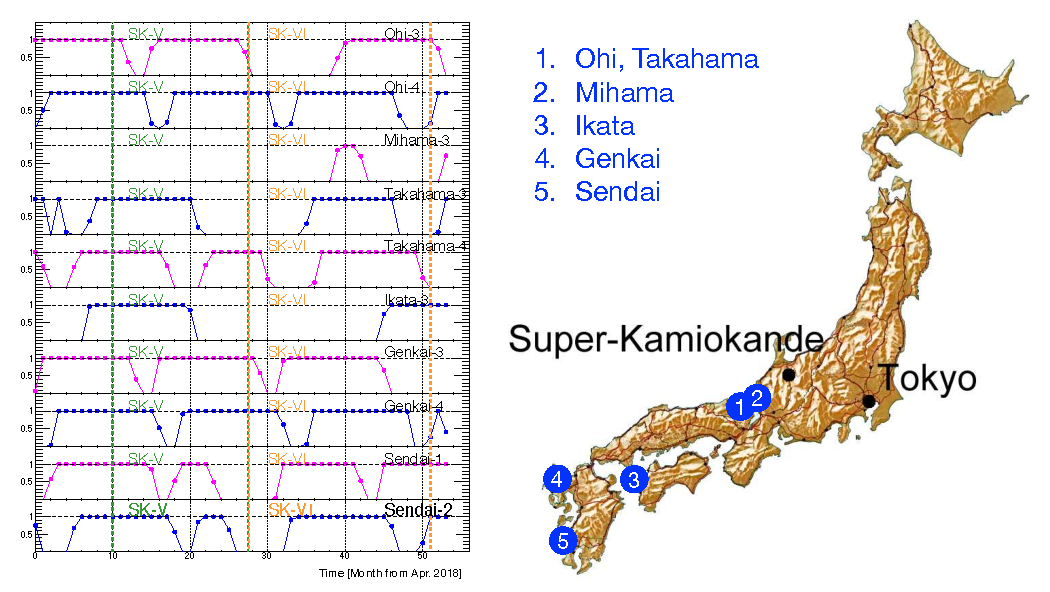
\includegraphics[width=12cm]{Figures/Simulation/Reactor_act}
	\caption[Activities of Japanese reactors from April 2018]{
	Activities of Japanese reactors from April 2018~\cite{2003Fukuda,2023HaradaPhD}.
	Dashed line shows the 100\% operation.
	Locations of nuclear power plants, Tokyo, and the SK are also shown in right side.
	}\label{Reactor_act}
\end{figure}

\begin{figure}[H]
	\centering
	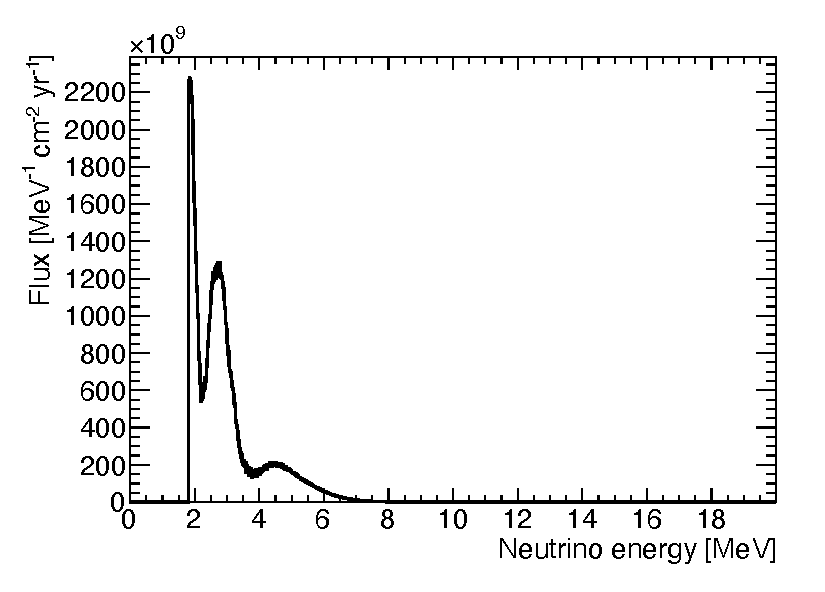
\includegraphics[width=8cm]{Figures/Simulation/Reactor_flux}
	\caption[Expected reactor neutrino flux at the SK]{
	Expected reactor neutrino flux at the SK~\cite{2023HaradaPhD}.
	In this flux, neutrino oscillation effect is considered.
	}\label{Reactor_flux}
\end{figure}

\begin{figure}[H]
	\centering
	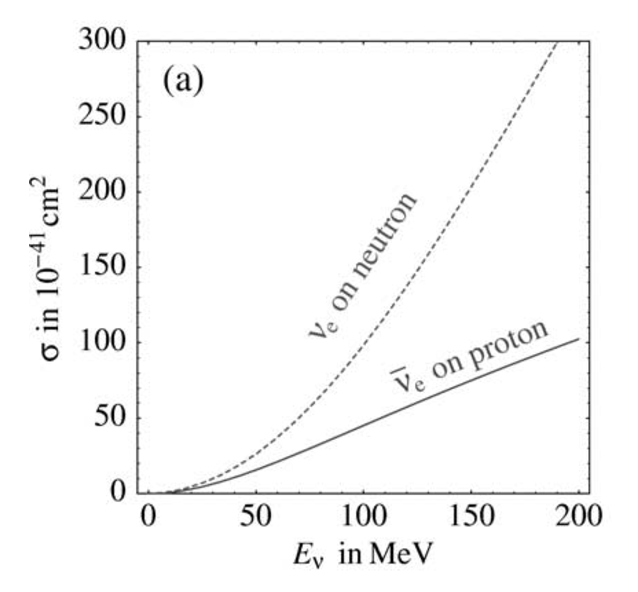
\includegraphics[width=6cm]{Figures/Simulation/IBD_XS}
	\caption[IBD cross section of Strumia-Vissani model]{
	IBD cross section of Strumia-Vissani model~\cite{2003Strumia}.
	}\label{IBD_XS}
\end{figure}

\subsubsection{DSNB events}
\vs\hs
As described in Section~\ref{Subsec_DSNBsearch}, DSNB events are the IBD events by electron antineutrinos.
The number of events is normalized by using the DSNB electron antineutrino flux (shown in Figure~\ref{Introd_DSNBpred}) and the IBD cross section of Strumia-Vissani model~\cite{2003Strumia} (shown in Figure~\ref{IBD_XS}).





\subsection{Detector simulation}
\vs\hs
In the past, a GEANT3-based~\cite{1994Brun} SK detector simulation (SKDETSIM, SK Detector Simulation) where only the Bertini Cascade Model (BERT) was implemented for neutron tracking in water was used.
However, a Geant4-based~\cite{2016Allison} (version 10.05.p01) SK detector simulation (SKG4, Super-Kamiokande Geant4 based Simulation) has been newly developed for the SK-Gd experiment.
In this simulation, BERT ({\tt \verb|FTFP_BERT_HP|} physics list), the Binary Cascade Model (BIC) ({\tt \verb|QGSP_BIC_HP|} physics list), and the Li$\grave{\text{e}}$ge Intranuclear Cascade model (INCL++) ({\tt \verb|QGSP_INCLXX_HP|} physics list) can be used as the secondary interaction model.
Here, BERT is a traditional cascade model used in GEANT.
BIC uses a large set of hadron data to choose interaction processes to improve the accuracy.
INCL++ is an advanced binary cascade model including phase space and quantum mechanical processes.
The features of each secondary interaction model are described in Section~\ref{Subsec_Features}.
In this NCQE cross section measurement, BERT is used as the baseline model.\\
\hs
Figure~\ref{model_ninel}, Figure~\ref{model_pinel}, and Figure~\ref{model_piinel} show the final state models of inelastic scattering for neutron, proton, and charged pion, respectively.
As described in Section~\ref{Subsec_NCQEbackground}, knocked-out neutrons of NCQE events may have hundreds of MeV, and neutrons with hundreds of MeV follow BERT, BIC, or INCL++ model as shown in Figure~\ref{model_ninel}.
Therefore, it is important to understand the difference among these models and select an appropriate model.\\
\hs
As shown in Figure~\ref{model_piinel}, when the kinetic energy (momentum) of incoming charged pion is below 379.544~(500)~MeV, NEUT model is used.
At the energy range, cross sections of charged pion inelastic scattering are also replaced to those of NEUT.
Figure~\ref{XS_piinel} shows the cross sections of charged pion inelastic scattering.\\
\hs
Gamma-rays emitted from thermal neutron capture on Gd are based on ANNRI-Gd model~\cite{2020Tanaka}.
Here, ANNRI stands for the Accurate Neutron-Nucleus Reaction Measurement Instrument.
Figure~\ref{Simula_RatioGdGam} shows the ratio of data from the ANNRI experiment to MC with the ANNRI-Gd model for the single gamma-ray events~\cite{2020Tanaka}.
As shown in this figure, the ANNRI-Gd model shows good agreement with the data.

\begin{figure}[H]
	\centering
	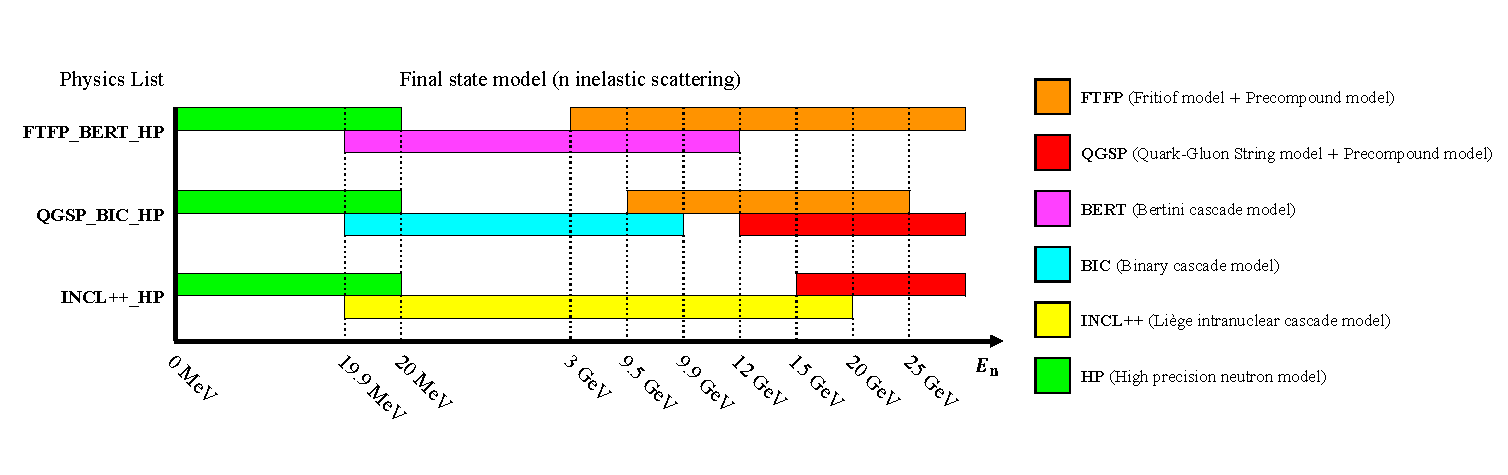
\includegraphics[width=16cm]{Figures/Simulation/model_ninel}
	\caption[Final state models of neutron inelastic scattering]{
	Final state models of neutron inelastic scattering.
	Horisontal axis represents the kinetic energy of incoming neutron.
	}\label{model_ninel}
\end{figure}

\begin{figure}[H]
	\centering
	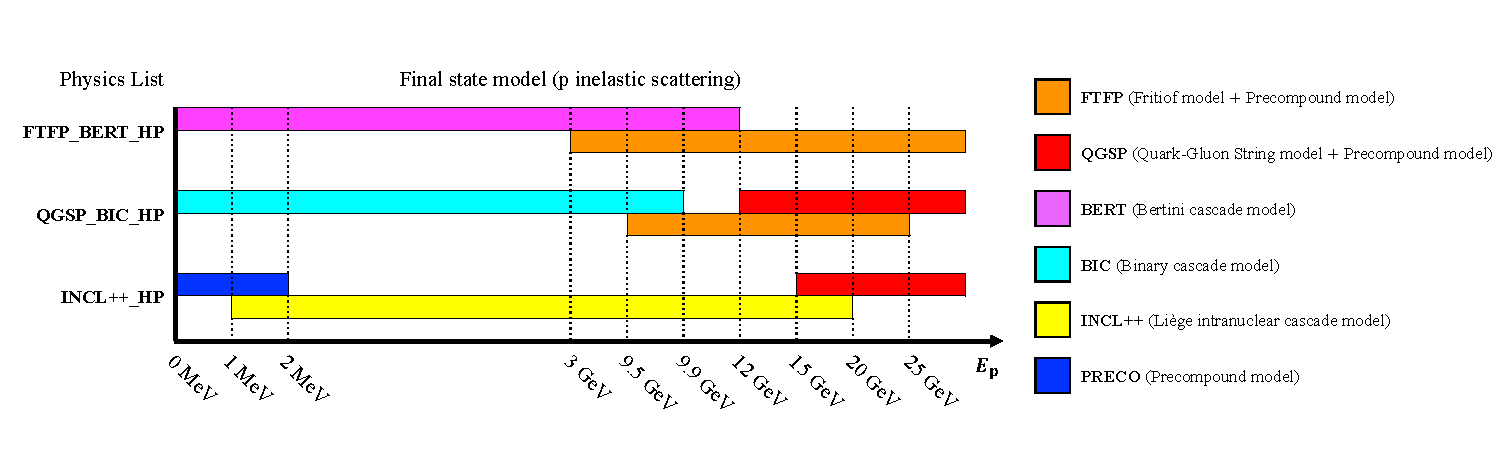
\includegraphics[width=16cm]{Figures/Simulation/model_pinel}
	\caption[Final state models of proton inelastic scattering]{
	Final state models of proton inelastic scattering.
	Horisontal axis represents the kinetic energy of incoming proton.
	}\label{model_pinel}
\end{figure}

\begin{figure}[H]
	\centering
	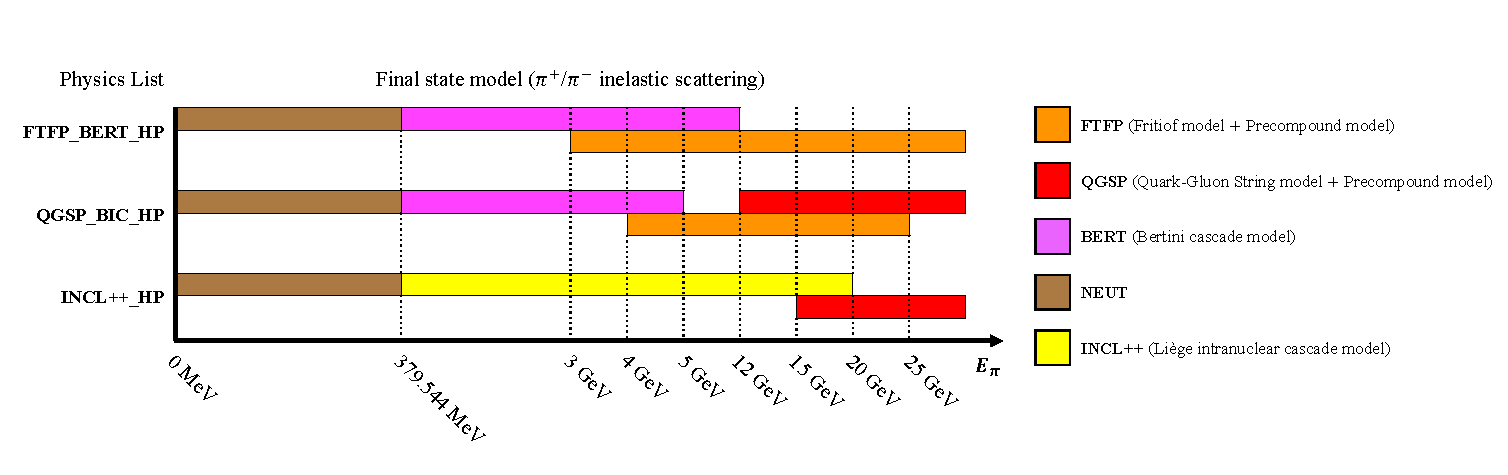
\includegraphics[width=16cm]{Figures/Simulation/model_piinel}
	\caption[Final state models of charged pion inelastic scattering]{
	Final state models of charged pion inelastic scattering.
	Horisontal axis represents the kinetic energy of incoming charged pion.
	}\label{model_piinel}
\end{figure}

\begin{figure}[tbp]
	\centering
	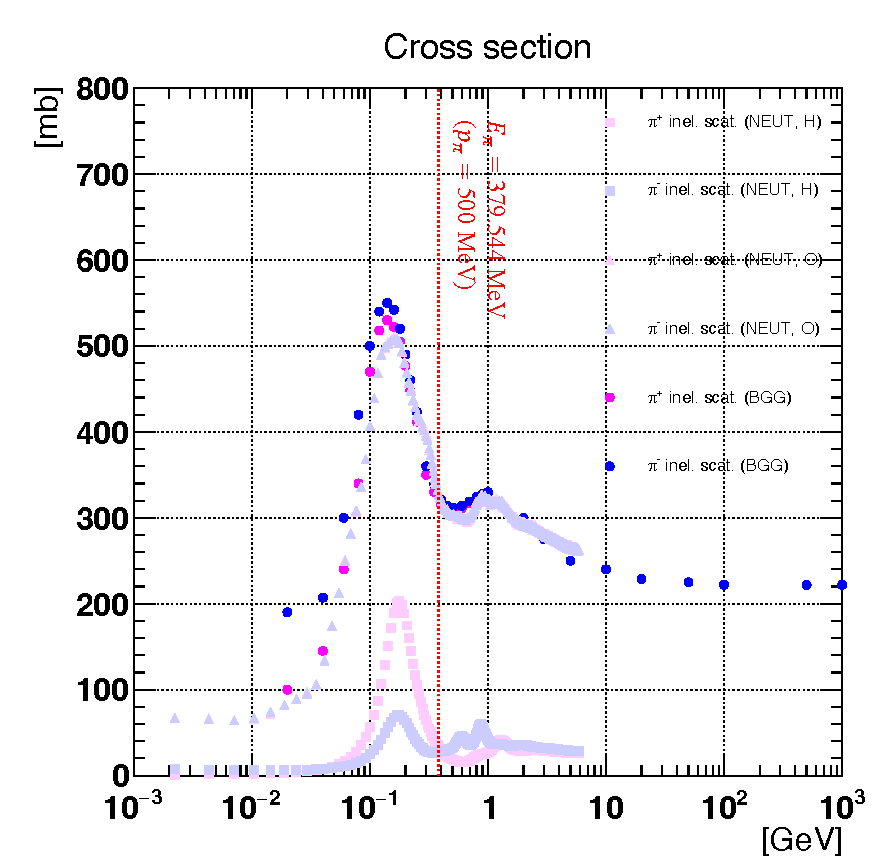
\includegraphics[width=10cm]{Figures/Simulation/XS_piinel}
	\caption[Cross sections of charged pion inelastic scattering]{
	Cross sections of charged pion inelastic scattering.
	Horisontal axis shows the kinetic energy of incoming charged pion.
	BGG stands for Barashenkov-Glauber-Gribov.
	}\label{XS_piinel}
\end{figure}

\begin{figure}[tbp]
	\centering
	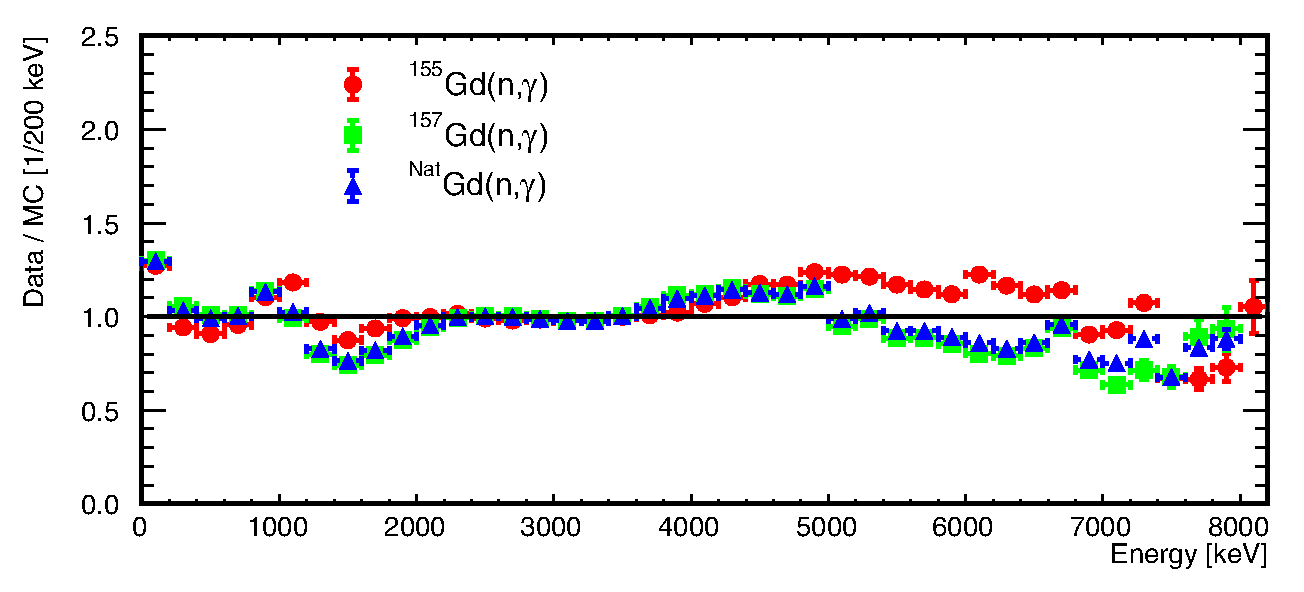
\includegraphics[width=10cm]{Figures/Simulation/RatioGdGam}
	\caption[Ratio of data from the ANNRI experiment by MC with the ANNRI-Gd model for the single gamma-ray events]{
	Ratio of data from the ANNRI experiment to MC with the ANNRI-Gd model for the single gamma-ray events~\cite{2020Tanaka}.
	}\label{Simula_RatioGdGam}
\end{figure}





\newpage



%	Event reconstruction

\section{Event reconstruction}\label{Section_Reconstruction}
\Headerfooter{Event reconstruction}
\subsection{Vertex reconstruction}\label{Subsec_vertex_rec}
\vs\hs
A charged particle with the energy of $\mathcal{O}$(10)~MeV travel a few centimeters in water.
Since vertex resolution is worse than track length of the charged particle due to the detector size and time resolution of PMTs, track length of the charged particle can be treated as a point.
Vertex is reconstructed by using a maximum-likelihood method.
The likelihood function is defined as
\begin{eqnarray}
	\mathcal{L}(\bm{x},t_{0}) &=& \sum_{i=1}^{N_{\rm hit}} \log P(t_{{\rm res},i}), \\
	t_{{\rm res},i}           &=& t_{i} - t_{0} - {|\bm{x} - \bm{h}_{i}| \over c},
\end{eqnarray}
where $\bm{x} = (x,y,z)$ is the candidate vertex, $t_{0}$ is the time when a charged particle was generated, $N_{\rm hit}$ is the number of hit PMTs, $t_{{\rm res},i}$ is the timing residual, $P(t_{{\rm res},i})$ is the probability density function for $t_{{\rm res},i}$, $t_{i}$ is the PMT's hit time, $\bm{h}_{i}$ is the position of hit PMT, and $c$ is the group velocity of light in water.
$t_{0}$ is fitted to minimize all $t_{{\rm res},i}$.
Figure~\ref{Recons_SK_coordinate} and Figure~\ref{Recons_PDF_vertex} shows the definition of the SK detector coordinate system~\cite{2016Abe} and the probability density function for $t_{{\rm res},i}$~\cite{2023HaradaPhD}, respectively.
Moreover, vertex resolution for SK-I, II, III, and IV is shown in Figure~\ref{Recons_Res_vertex}~\cite{2016Abe}.

\begin{figure}[h]
	\centering
	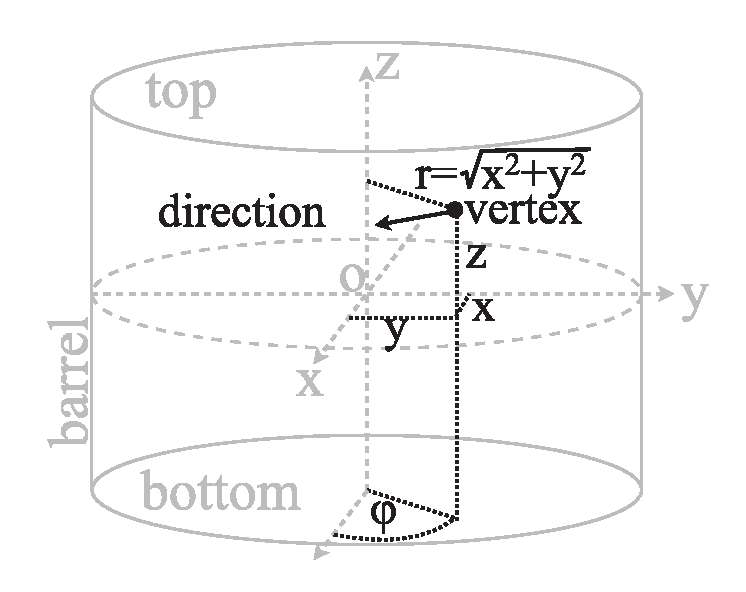
\includegraphics[width=6cm]{Figures/Reconstruction/SK_coordinate}
	\caption[Definition of the SK detector coordinate system]{
	Definition of the SK detector coordinate system~\cite{2016Abe}.
	}\label{Recons_SK_coordinate}
\end{figure}

\begin{figure}[h]
	\centering
	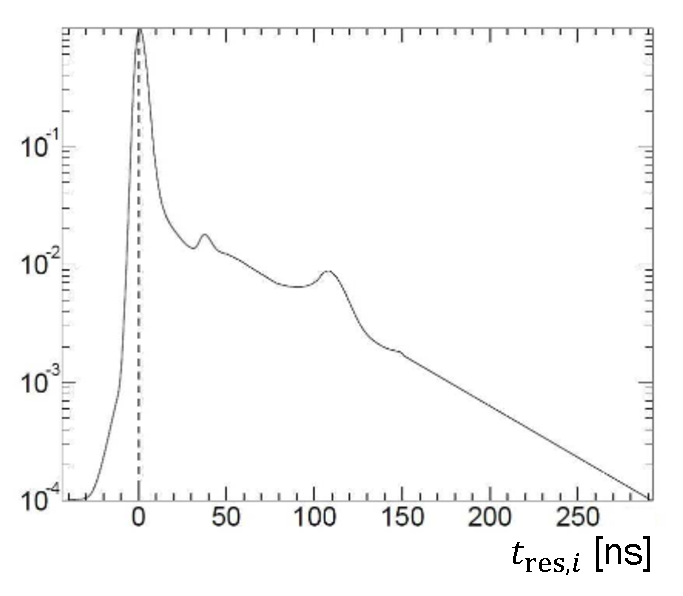
\includegraphics[width=8cm]{Figures/Reconstruction/PDF_vertex}
	\caption[Probability density function for $t_{{\rm res},i}$]{
	Probability density function for $t_{{\rm res},i}$~\cite{2023HaradaPhD}.
	Peaks around 40~ns and 110~ns come from after pulses of PMTs.
	}\label{Recons_PDF_vertex}
\end{figure}

\begin{figure}[tbp]
	\centering
	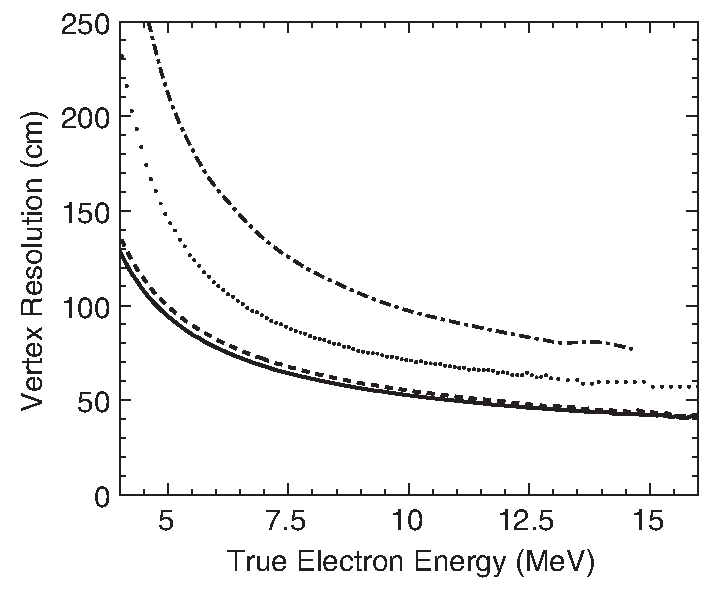
\includegraphics[width=8cm]{Figures/Reconstruction/Res_vertex}
	\caption[Vertex resolution for SK-I, II, III, and IV]{
	Vertex resolution for SK-I, II, III, and IV~\cite{2016Abe}.
	Dotted, dashed-dotted, dashed, and solid line shows that for SK-I, II, III, and IV, respectively.
	}\label{Recons_Res_vertex}
\end{figure}

\hs
The vertex reconstruction goodness, which is a parameter that indicates whether the vertex reconstruction is done well or not, is defined as
\begin{eqnarray}
	g_{\rm vtx} = {\displaystyle \sum_{i=1}^{N_{\rm hit}} \bigg[\exp\bigg\{-\bigg({t_{{\rm res},i} \over \sqrt{2}\omega}\bigg)^{2}\bigg\}\exp\bigg\{-\bigg({t_{{\rm res},i} \over \sqrt{2}\sigma}\bigg)^{2}\bigg\}\bigg] \over \displaystyle \sum_{i=1}^{N_{\rm hit}} \exp\bigg\{-\bigg({t_{{\rm res},i} \over \sqrt{2}\omega}\bigg)^{2}\bigg\}},
\end{eqnarray}
where $\omega$ is the resolution of the $t_{{\rm res},i}$ distribution and $\sigma$ is the timing resolution of PMTs.
The range of $g_{\rm vtx}$ is from 0 to 1, and the value is close to 1 when the vertex reconstruction is done well.





\subsection{Direction reconstruction}\label{Subsec_direction_rec}
\vs\hs
After determining the vertex, direction is reconstructed.
Direction is reconstructed by using a maximum-likelihood method with hit PMTs within 20~ns.
The likelihood function is defined as
\begin{eqnarray}
	\mathcal{L}(\bm{d}) = \sum_{i=1}^{N_{20}} \bigg[\log f(\cos\Theta_{i},E) \times {\cos\theta_{i} \over a(\theta_{i})}\bigg],
\end{eqnarray}
where $\bm{d}$ is the candidate direction, $N_{20}$ is the number of hit PMTs within 20~ns, $\Theta_{i}$ is the angle between the candidate direction and the direction from the reconstructed vertex to the position of hit PMT, $f(\cos\Theta_{i},E)$ is the probability density function for $\cos\Theta_{i}$ depending on the energy $E$, $\theta_{i}$ is the angle between the direction from the reconstructed vertex to the position of hit PMT and the direction in which the hit PMT is oriented, and $a(\theta_{i})$ is the correction function of PMT acceptance.
$a(\theta_{i})$ is defined as
\begin{eqnarray}\label{Recons_Eq_a_theta}
	a(\theta_{i}) = 0.205 + 0.524\cos\theta_{i} + 0.390\cos^{2}\theta_{i} - 0.132\cos^{3}\theta_{i}.
\end{eqnarray}
Figure~\ref{Recons_PDF_direction} shows the probability density function for $\cos\Theta_{i}$ depending on the energy $E$~\cite{2011Abe}.
Moreover, Figure~\ref{Recons_Res_direction} shows the angular resolution for SK-I and SK-III~\cite{2011Abe}.

\begin{figure}[tbp]
	\centering
	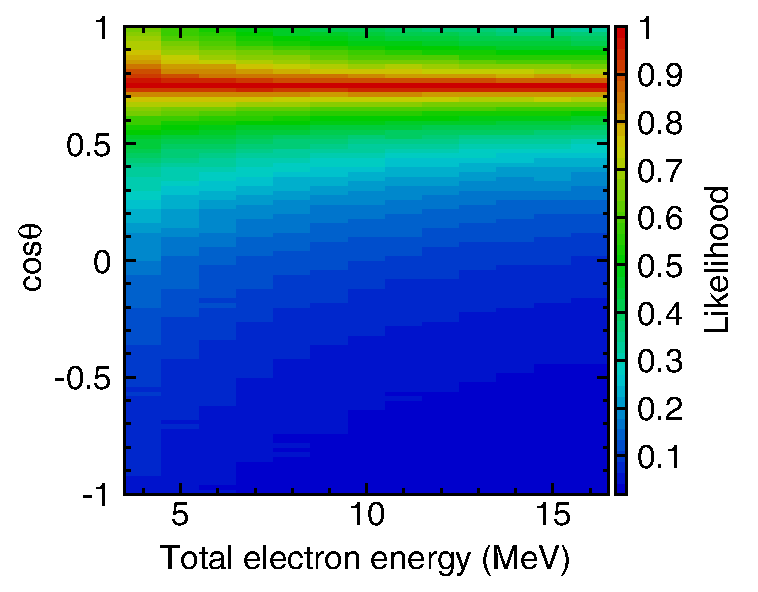
\includegraphics[width=8cm]{Figures/Reconstruction/PDF_direction}
	\caption[Probability density function for $\cos\Theta_{i}$ depending on the energy $E$]{
	Probability density function for $\cos\Theta_{i}$ depending on the energy $E$~\cite{2011Abe}.
	}\label{Recons_PDF_direction}
\end{figure}

\begin{figure}[tbp]
	\centering
	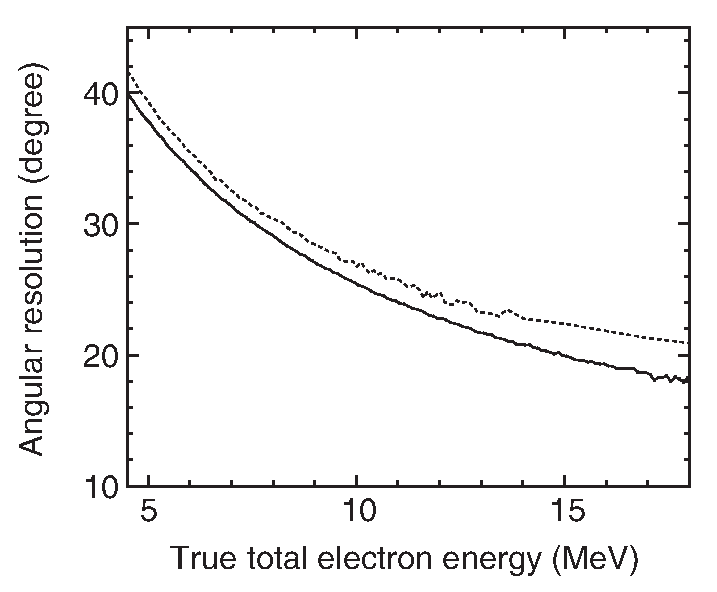
\includegraphics[width=8cm]{Figures/Reconstruction/Res_direction}
	\caption[Angular resolution for SK-I and SK-III]{
	Angular resolution for SK-I and SK-III~\cite{2011Abe}.
	Dashed and solid line shows that for SK-I and SK-III, respectively.
	}\label{Recons_Res_direction}
\end{figure}

\hs
The direction reconstruction goodness, which is a parameter that indicates whether the direction reconstruction is done well or not, is defined as
\begin{eqnarray}
	g_{\rm dir} = {1 \over 2\pi}\bigg\{{\rm max}\bigg(\phi_{i} - {2\pi \times i \over N_{\rm hit}}\bigg) - {\rm min}\bigg(\phi_{i} - {2\pi \times i \over N_{\rm hit}}\bigg)\bigg\},
\end{eqnarray}
where $\phi_{i}$ is the azimuthal angle of the $i$-th hit PMT.
The range of $g_{\rm dir}$ is from 0 to 1, and the value is close to 0 when the direction reconstruction is done well.





\subsection{Energy reconstruction}
\vs\hs
Energy is reconstructed by using $N_{\rm eff}$, which does not depend on vertex, direction, the number of bad-channel PMTs, water transparency, and relative quantum efficiency (QE) of each PMT.
$N_{\rm eff}$ is defined as
\begin{eqnarray}\label{Eq_Recons_Neff}
	N_{\rm eff} = \sum_{i=1}^{N_{50}} \biggl[(X_{i} + \epsilon_{\rm tail} - \epsilon_{\rm dark}) \times {N_{\rm all} \over N_{\rm alive}} \times {S(0,0) \over S(\theta_{i},\phi_{i})} \times \exp\biggl({r_{i} \over L_{\rm eff}^{i}}\biggr) \times {1 \over QE_{i}}\biggr],
\end{eqnarray}
where $N_{50}$ is the number of hit PMTs within 50~ns.
Parameters shown in Equation~(\ref{Eq_Recons_Neff}) is described below.\\

\textbf{$X_{i}$ : Correction for multiple hits}\\
\hs
When an event occur at the edge of fiducial volume or an event is caused by a charged particle with high energy, multiple photons may hit a PMT nearby the vertex.
The multiple hits are corrected by using $X_{i}$ defined as
\begin{eqnarray}
	X_{i} &=&
	\left\{
	\begin{array}{ll}
		\displaystyle {\log\{1/(1 - n_{i}/N_{i})\} \over n_{i}/N_{i}} & (n_{i}/N_{i} < 1) \\
		3.0                                                           & (n_{i}/N_{i} = 1)
	\end{array} \right.,
\end{eqnarray}
where $N_{i}$ is the number of PMTs adjacent to the hit PMT and $n_{i}$ is the number of hits in the adjacent PMTs.\\

\textbf{$\epsilon_{\rm tail}$ : Correction for scattering and reflection}\\
\hs
Cherenkov photons scattering in water or reflecting at the surface of PMT or black sheet may hit a PMT at time out of a time width of 50~ns.
The effects of scattering and reflection are corrected by using $\epsilon_{\rm tail}$ defined as
\begin{eqnarray}
	\epsilon_{\rm tail} = {N_{100} - N_{50} - N_{\rm alive} \times R_{\rm dark} \times 50\,{\rm ns} \over N_{50}},
\end{eqnarray}
where $N_{100}$ is the number of hit PMTs within 100~ns, $N_{\rm alive}$ is the number of alive PMTs and $R_{\rm dark}\,({\rm hits}/{\rm ns})$ is the dark-noise rate at a period.\\

\textbf{$\epsilon_{\rm dark}$ : Correction for dark-noise hits}\\
\hs
Hits caused by PMT dark noise may enter the time width of 50~ns.
The dark-noise hits, which are not originated from Cherenkov photons, are corrected by using $\epsilon_{\rm dark}$ defined as
\begin{eqnarray}
	\epsilon_{\rm dark} = {N_{\rm alive}\times R_{\rm dark} \times 50\,{\rm ns} \over N_{50}} \times {R_{\rm dark}^{i} \over \displaystyle \sum_{i=1}^{N_{50}} {R_{\rm dark}^{i} \over N_{50}}},
\end{eqnarray}
where $R_{\rm dark}^{i}\,({\rm hits}/{\rm ns})$ is the dark-noise rate of the $i$-th hit PMT at a period.\\

\textbf{$N_{\rm all}/N_{\rm alive}$ : Correction for bad-channel PMTs}\\
\hs
If there is a PMT that does not work properly, the number of hits would be underestimated and energy would not be reconstructed correctly.
The effects of bad-channel PMTs are corrected by multiplying $N_{\rm all}/N_{\rm alive}$, where $N_{\rm all}\,(= 11{,}129)$ is the number of all PMTs.\\

\textbf{$S(0,0)/S(\theta_{i},\phi_{i})$ : Correction for change of photo coverage by the incident angle of photon}\\
\hs
Photo coverage changes depending on the incident angle of a Cherenkov photon.
This effect is corrected by using the correction function $S(\theta_{i},\phi_{i})$.
Figure~\ref{Recons_PMT_theta_phi} and Figure~\ref{Recons_PMTCorrFunc} show the definition of the incident angle and distributions of correction function $S(\theta_{i},\phi_{i})$ for barrel PMTs and top and bottom PMTs, respectively.\\

\begin{figure}[h]
	\centering
	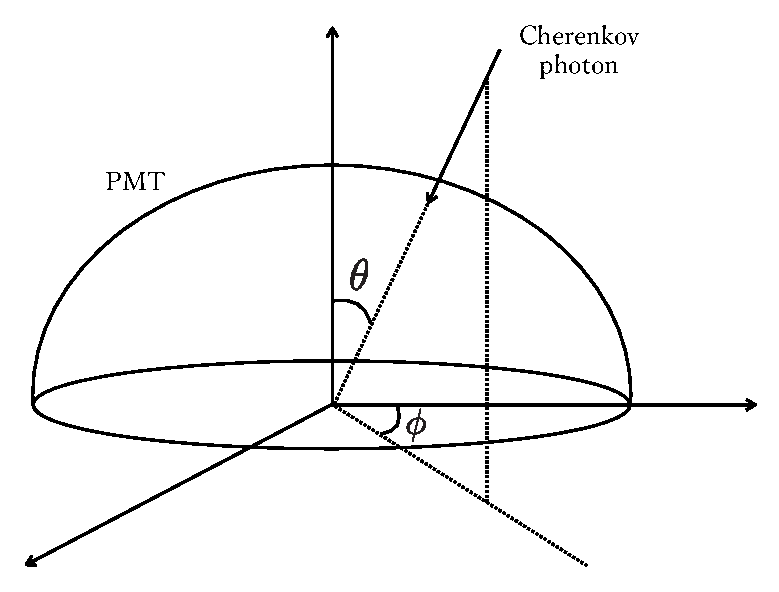
\includegraphics[width=8cm]{Figures/Reconstruction/PMT_theta_phi}
	\caption[Definition of the incident angle]{
	Definition of the incident angle~\cite{2021ShinokiMas}.
	}\label{Recons_PMT_theta_phi}
\end{figure}

\begin{figure}[h]
	\centering
	\includegraphics[width=16cm]{Figures/Reconstruction/PMTCorrFunc}
	\caption[Distributions of correction function $S(\theta_{i},\phi_{i})$ for barrel PMTs and top and bottom PMTs]{
	Distributions of correction function $S(\theta_{i},\phi_{i})$ for barrel PMTs (left) and top and bottom PMTs (right)~\cite{2021ShinokiMas}.
	}\label{Recons_PMTCorrFunc}
\end{figure}

\textbf{$\exp(r_{i}/L_{\rm eff}^{i})$ : Correction for water transparency}\\
\hs
Cherenkov photons may be scattered or absorbed in water before arriving at a PMT.
The probability that a Cherenkov photon arrives at a PMT can be written as $\exp(-r_{i}/L_{\rm eff}^{i})$, where $r_{i}$ is the distance from the vertex to a hit PMT and $L_{\rm eff}^{i}$ is the effective attenuation length, which is described below.
Therefore, the effect of water transparency is corrected by multiplying $\exp(r_{i}/L_{\rm eff}^{i})$.\\
\hs
$L_{\rm eff}^{i}$ is expressed as
\begin{eqnarray}
	L_{\rm eff}^{i} = -{r_{i} \over {\rm ln}\Bigg[\displaystyle \int_{\lambda_{\rm min}}^{\lambda_{\rm max}} w_{0}(\lambda)\exp\{-\sigma_{i}(\lambda) \times r_{i}\} d\lambda\Bigg]},
\end{eqnarray}
where $\lambda_{\rm min} = 300\,{\rm nm}$, $\lambda_{\rm max} = 650\,{\rm nm}$, $w_{0}(\lambda)$ is the probability density function for wavelength $\lambda$ of Cherenkov photons (shown in Figure~\ref{Recons_PDF_wavelength}), and $\sigma_{i}(\lambda)$ is the cross section with water when a Cherenkov photon travels a distance $r_{i}$.
$\sigma_{i}(\lambda)$ is expressed as
\begin{eqnarray}
	\sigma_{i}(\lambda) = \alpha_{\rm abs}(\lambda)\bigg\{1 + \beta\bigg(z + {1 \over 2}r_{i} \times dz_{i}\bigg)\bigg\} + C_{\rm sca}\{\alpha_{\rm sym}(\lambda) + \alpha_{\rm asy}(\lambda)\},
\end{eqnarray}
where $z$ is the z position of the vertex, $dz_{i}$ is the z component of direction to the hit PMT, and $C_{\rm sca} (\sim 0.44)$ is the correction factor of the scattering effect.
$C_{\rm sca}$ was estimated to minimize the position dependence of $N_{\rm eff}$ using the SK detector simulation.
$\alpha_{\rm abs}(\lambda)$, $\alpha_{\rm sym}(\lambda)$, and $\alpha_{\rm asy}(\lambda)$ are the attenuation coefficients of absorption, symmetric scattering, and asymmetric scattering at wavelength $\lambda$, respectively, and $\beta$ is the parameter indicating the degree of z dependence in water quality.
Details about $\alpha_{\rm abs}(\lambda)$, $\alpha_{\rm sym}(\lambda)$, $\alpha_{\rm asy}(\lambda)$, and $\beta$ are described in Section~\ref{Subsubsec_Water}.

\begin{figure}[h]
	\centering
	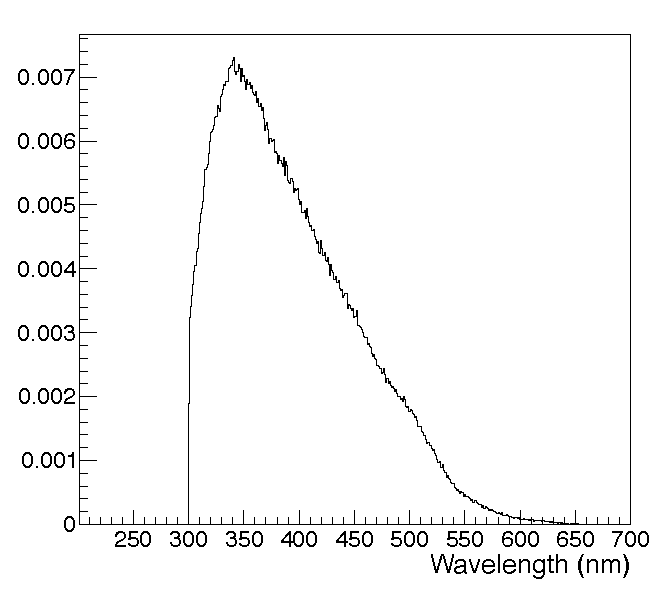
\includegraphics[width=8cm]{Figures/Reconstruction/PDF_wavelength}
	\caption[Probability density function for wavelength $\lambda$ of Cherenkov photons]{
	Probability density function for wavelength $\lambda$ of Cherenkov photons~\cite{2021ShinokiMas}.
	}\label{Recons_PDF_wavelength}
\end{figure}

\textbf{$1/QE_{i}$ : Correction for relative QE of each PMT}\\
\hs
QE differs for each PMT.
The effect of QE is corrected by multiplying $1/QE_{i}$, where $QE_{i}$ is the relative QE of the hit PMT.
Details about $QE_{i}$ are described in Section~\ref{Subsubsec_QE}.\\
\\
\hs
Visible energy of the prompt signal ($E_{\rm vis}$) is determined by using $N_{\rm eff}$.
Relation between $E_{{\rm vis}}$ and $N_{\rm eff}$ is expressed as 
\begin{eqnarray}
	E_{\rm vis} =
	\left\{
	\begin{array}{ll}
		\displaystyle \sum_{i=0}^{5} p_{i}(N_{\rm eff})^{i}                                                                                 & (N_{\rm eff} \leq N_{\rm thr}) \\
		\displaystyle \sum_{i=0}^{5} p_{i}(N_{\rm thr})^{i} + (N_{\rm eff} - N_{\rm thr}) \times \sum_{i=1}^{5} ip_{i}(N_{\rm thr})^{i - 1} & (N_{\rm eff} > N_{\rm thr})
	\end{array} \right..
\end{eqnarray}
The values of $p_{i}$ and $N_{\rm thr}$ are summarized in Table~\ref{tab:Recons_Neff}.

\begin{table}[H]
	\centering
	\caption[Values of $p_{i}$ and $N_{\rm thr}$]{
	Values of $p_{i}$ and $N_{\rm thr}$~\cite{2023HaradaPhD}.
	}\label{tab:Recons_Neff}
	\vs
	\begin{tabular}{cc} \hline \hline
		$p_{0}$       & $0.702$                 \\
		$p_{1}$       & $0.131$                 \\
		$p_{2}$       & $-2.35 \times 10^{-4}$  \\
		$p_{3}$       & $2.640 \times 10^{-6}$  \\
		$p_{4}$       & $-1.188 \times 10^{-8}$ \\
		$p_{5}$       & $1.930 \times 10^{-11}$ \\
		$N_{\rm thr}$ & $2.202 \times 10^{2}$   \\ \hline \hline
	\end{tabular}
\end{table}





\newpage



%
%	Calibration
%

\section{Calibration}\label{Section_Calibration}
\Headerfooter{Calibration}

\subsection{ID detector calibration}
\vs\hs ID detector calibration!

\begin{figure}[tbp]
	\centering
	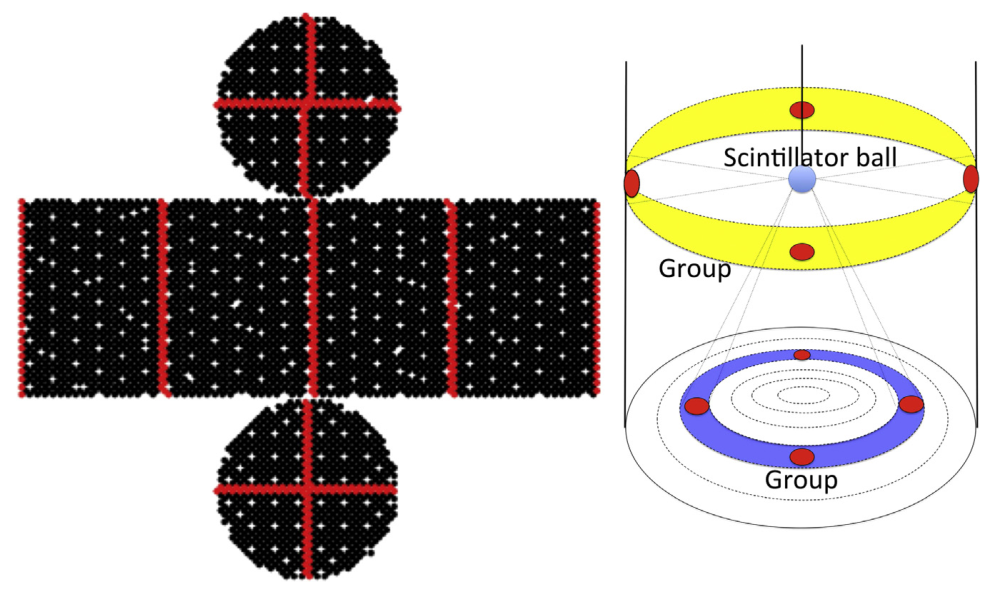
\includegraphics[width=10cm]{Figures/Calibration/CalibPMT}
	\caption[Location of standard PMTs in ID and schematic view of the groups of PMTs]{\label{Calibration_CalibPMT} Location of standard PMTs in ID (left) and schematic view of the groups of PMTs (right)~\cite{2014AbeCalib}.}
\end{figure}

\begin{figure}[tbp]
	\centering
	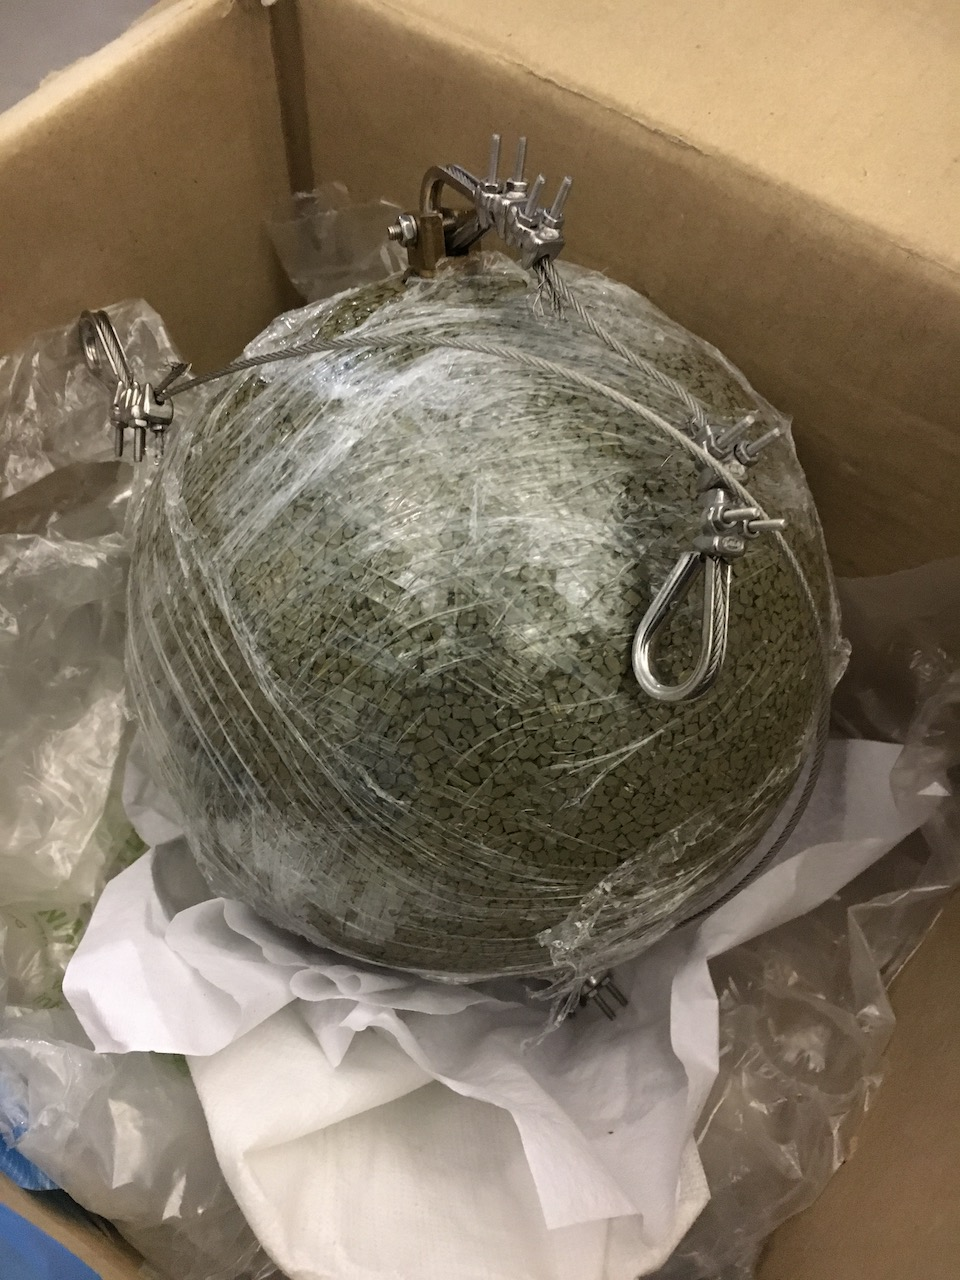
\includegraphics[width=6cm]{Figures/Calibration/Ni}
	\caption[Picture of the Ni-Cf source]{\label{Calibration_Ni} Picture of the Ni-Cf source.}
\end{figure}

\begin{figure}[tbp]
	\centering
	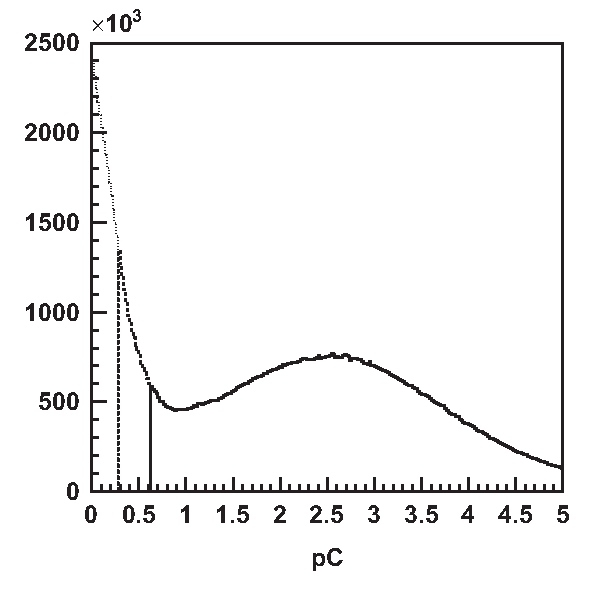
\includegraphics[width=8cm]{Figures/Calibration/Single-pe}
	\caption[Single-pe distribution of the Ni-Cf source data in SK-III]{\label{Calibration_Single-pe} Single-pe distribution of the Ni-Cf source data in SK-III~\cite{2014AbeCalib}. The dashed line shows the data with double gain and half threshold. The dotted line is linear extrapolation.}
\end{figure}

\begin{figure}[tbp]
	\centering
	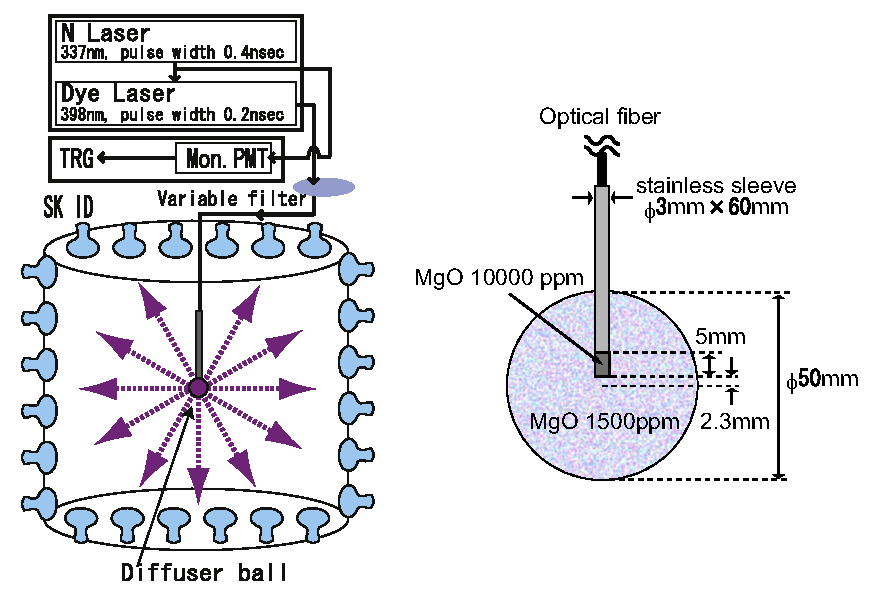
\includegraphics[width=10cm]{Figures/Calibration/TimingCalib}
	\caption[Schematic view of the timing calibration system and cross section of the diffuser ball]{\label{Calibration_TimingCalib} Schematic view of the timing calibration system (left) and cross section of the diffuser ball (right)~\cite{2014AbeCalib}.}
\end{figure}

\begin{figure}[tbp]
	\centering
	\includegraphics[width=10cm]{Figures/Calibration/TQ}
	\caption[Timing and charge distribution for a readout channel]{\label{Calibration_TQ} Timing and charge distribution for a readout channel~\cite{2014AbeCalib}. Horizontal axis shows charge (QBin) of each hit. Vertical axis shows TOF-corrected hit timing.}
\end{figure}

\begin{figure}[tbp]
	\centering
	\includegraphics[width=12cm]{Figures/Calibration/LaserCalib}
	\caption[Schematic view of the laser calibration system and TOF-subtracted timing distributions of the laser calibration data and MC]{\label{Calibration_LaserCalib} Schematic view of the laser calibration system (left) and TOF-subtracted timing distributions of the laser calibration data and MC (right)~\cite{2014AbeCalib}. Water parameter tuning is performed using top PMTs that are 2 m away from the laser light injector, and barrel PMTs. Barrel is separated into five regions, from B1 to B5. B3 includes PMTs for 11 lines and the others include PMTs for 10 lines. In the left figure, the cyan shaded circle spot on the bottom shows the beam target used in the TOF calculation. In the right figure, the black circle shows data and the red histogram shows MC. Both data and MC are normalized by observed total photoelectrons. Time region between the left two blue solid vertical lines is used for the water parameter tuning. Right time region is used for the PMT reflectivity measurement.}
\end{figure}

\begin{figure}[tbp]
	\centering
	\includegraphics[width=10cm]{Figures/Calibration/CalibBS}
	\caption[Schematic view of the black sheet reflectivity measurement]{\label{Calibration_CalibBS} Schematic view of the black sheet reflectivity measurement~\cite{2014AbeCalib}. Left figure shows the top view. The laser light injector is inserted from the top center of the SK tank and the reflected light is measured by ID PMTs.}
\end{figure}

\newpage


%	Event selection

\section{Event selection}\label{Section_Selection}
\Headerfooter{Event selection}
\vs\hs
In this study, we search for NCQE events that consist of prompt signals from de-excitation gamma-rays and delayed signals from neutrons.
We select events where the visible energy of the prompt signal ($E_{{\rm vis}}$) is between 7.49~MeV and 29.49~MeV because most NCQE events are in the $E_{{\rm vis}}$ region (see Figure~\ref{FTFP_BERT_HP_Figure08_Poisson}).
In each candidate event, delayed signals within 535 $\mu$s from the prompt signal are searched.
The event reconstruction and neutron tagging method follow the DSNB search in SK-Gd phase~\cite{2023Harada,2022Harada}.
%Details of the neutron tagging method are summarized in Section~6 of Ref.~\cite{2023HaradaPhD}.\\
Details of the neutron tagging method are summarized in Section~\ref{Subsubsec_Ndelayed}.\\
\hs
The data sample includes not only NCQE events but also other events such as atmospheric neutrino NC non-QE events, atmospheric neutrino charged-current (CC) events, spallation events (see Section~\ref{Subsubsec_sim_spa}), reactor neutrino events (see Section~\ref{Subsubsec_sim_reactor}), and accidental coincidence events.
Most of atmospheric neutrino NC non-QE events ($\sim$90.4\% of NC non-QE events after applying all event selections) are events with single meson, as shown in Figure~\ref{Selection_NC_single_meson}.
Schematic view of atmospheric neutrino CC events is shown in Figure~\ref{Selection_CC_nue_CC_numu}.
Muon neutrino CC events become backgrounds when the emitted muon is invisible (below Cherenkov threshold (see Section~\ref{subsec_detect_princi})).
Accidental coincidence events are mainly pairs of a spallation event without neutrons and a neutron misidentification event.
Most of these events can be removed by applying various event reductions.
However, some events remain even after applying all event reductions.
To determine the number of NCQE events, it is necessary to estimate the number of all those events.
The methods of event reduction and event estimation are described below.\\
\hs
This study uses 552.2~days of data with 0.011\% gadolinium-loaded water from August 2020 to June 2022.
This data set is the same as the one used for the SK-Gd DSNB search~\cite{2023Harada}.

\begin{figure}[h]
	\centering
	\includegraphics[width=6cm]{Figures/Selection/NC_single_meson}
	\caption[Schematic view of an atmospheric neutrino NC event with single meson]{
	Schematic view of an atmospheric neutrino NC event with single meson.
	}\label{Selection_NC_single_meson}
\end{figure}

\begin{figure}[h]
	\centering
	\includegraphics[width=12cm]{Figures/Selection/CC_nue_CC_numu}
	\caption[Schematic view of atmospheric neutrino CC events]{
	Schematic view of atmospheric neutrino CC events.
	}\label{Selection_CC_nue_CC_numu}
\end{figure}





\subsection{First reduction: Pre-cut}
\subsubsection{Non-SHE-triggered event and noise event cut}
\vs\hs
First, when a run satisfies the following conditions, events in the run are not used.
\begin{itemize}
	\item Run time is shorter than 5~minutes
	\item Run started less than 15~minutes after the high-voltage was recovered
	\item Any hardware problem is reported
	\item Event distribution is unusual due to detector problems
\end{itemize}
\hs
Moreover, the following events are removed.
\begin{itemize}
	\item Calibration trigger events
	\item Periodic trigger events
	\item T2K beam trigger events
	\item Pedestal events
\end{itemize}
\hs
In addition, the condition $N(Q < 0.5\,{\rm p.e.})/N_{\rm total} < 0.55$ is required to remove the events triggered by PMT noise hits, where $N(Q < 0.5\,{\rm p.e.})$ is the number of hits with a charge smaller than $0.5\,{\rm p.e.}$ and $N_{\rm total}$ is the total number of hits.

\subsubsection{Cosmic ray muon-induced event cut}
\vs\hs
Cosmic ray muons come to the SK at $\sim$2~Hz, and most of these muons issue the OD trigger.
To remove events induced by cosmic ray muons, events that the OD trigger is issued are not used.
Moreover, some muons decay into electrons with a life time of 2.2~$\mu$s, leaving hits inside the ID without an OD trigger.
To remove events induced by these electrons, events within 50~$\mu$s from preceding cosmic ray muons are not used.
Spallation events caused by cosmic ray muons will be described later.

\subsubsection{Fiducial volume cut}
\vs\hs
Radioactive backgrounds are concentrated near the detector wall.
Therefore, events within 2~m away from the ID wall are removed.

\subsubsection{Fit quality cut}
\vs\hs
To remove poorly reconstructed events, events that the vertex reconstruction goodness ($g_{\rm vtx}$) is less than 0.5 are removed.
Details of $g_{\rm vtx}$ are summarized in Section~\ref{Subsec_vertex_rec}.

\subsubsection{Trigger requirement}
\vs\hs
To search delayed signals within 535~$\mu$s from the prompt signal, not only the SHE trigger but also the AFT trigger must be issued.
However, since the AFT trigger rate was limited to once every 21~ms until the middle of SK-VI, some events did not issue the AFT trigger.
Therefore, in MC, the number of events is scaled by using the AFT trigger efficiency $\varepsilon_{\rm AFT}$ defined as
\begin{eqnarray}
	\varepsilon_{\rm AFT} = {N_{\rm AFT} \over N_{\rm SHE}},
\end{eqnarray}
where $N_{\rm AFT}$ is the number of AFT-triggered events and $N_{\rm SHE}$ is the number of SHE-triggered events.
$\varepsilon_{\rm AFT}$ is summarized in Table~\ref{tab:AFT}.

\begin{table}[h]
	\centering
	\caption[AFT trigger efficiency considering the whole period of SK-VI]{
	AFT trigger efficiency considering the whole period of SK-VI.
	}\label{tab:AFT}
	\vs
	\begin{tabular}{cc} \hline \hline
		$E_{\rm vis}$ & $\varepsilon_{\rm AFT}$ \\
		(MeV)         &                         \\ \hline
		7.49--9.49    & 85.3\%                  \\
		9.49--11.49   & 80.4\%                  \\
		11.49--13.49  & 74.3\%                  \\
		13.49--15.49  & 70.0\%                  \\
		15.49--17.49  & 67.9\%                  \\
		17.49--19.49  & 63.4\%                  \\
		19.49--21.49  & 89.7\%                  \\
		21.49--23.49  & 90.0\%                  \\
		23.49--25.49  & 90.0\%                  \\
		25.49--27.49  & 100.0\%                 \\
		27.49--29.49  & 90.5\%                  \\ \hline \hline
	\end{tabular}
\end{table}





\subsection{Second reduction: Spallation cut}
\vs\hs
Here, the spallation events, which are major backgrounds in the energy range from a few MeV to tens of MeV, are removed.
As described in Section~\ref{Subsubsec_sim_spa}, some radioactive isotopes produced by cosmic-ray muon spallation of oxygen nuclei mimic the IBD and NCQE events.
The spallation cut consists of five components, and these components are described in Section~\ref{Sec_1ms} to Section~\ref{Sec_box}.

\subsubsection{1~ms cut}\label{Sec_1ms}
\vs\hs
Gamma-rays and neutrons are emitted by hadronic nuclear interactions caused by nucleons and mesons with hundreds of MeV generated by muon spallation.
In some cases, the gamma-rays can issue the SHE trigger, and the neutrons can be detected as delayed signals.
To remove these events, events within 1~ms from preceding cosmic ray muons are not used.

\subsubsection{Multiple spallation cut}
\vs\hs
Energetic cosmic ray muons may produce multiple radioactive isotopes.
When a spallation event issues the SHE trigger, other spallation events may be observed close to the event both in time and space.
To remove the SHE-triggered events, low energy events with a $E_{\rm vis}$ of 5.49--24.49~MeV within $\pm$60~s from the SHE-triggered event are used.
First, selection criteria of the solar neutrino analysis~\cite{2016Abe} are applied to all low energy events.
Then, the distance from the SHE-triggered event to each low energy event is calculated.
If there is one low energy event with a distance of less than 4.0~m, the SHE-triggered event is removed (see Figure~\ref{Selection_multiple_spa}).

\begin{figure}[h]
	\centering
	\includegraphics[width=12cm]{Figures/Selection/multiple_spa}
	\caption[Schematic view of multiple spallation cut]{
	Schematic view of multiple spallation cut.
	In this case, the SHE-triggered event is removed.
	}\label{Selection_multiple_spa}
\end{figure}

\subsubsection{Neutron cloud cut}
\vs\hs
Muon spallation produces many particles, including neutrons.
These neutrons are captured on Gd, and generate neutron event clusters, named neutron cloud, near the spallation point.
To remove spallation events, the information of neutron cloud is used.
First, the following selection criteria are applied to neutron events after muon spallation.
\begin{itemize}
	\item $N_{200} \geq 25$
	\item Timing is within [35, 535]~$\mu$s from the muon spallation
	\item $g_{\rm vtx} > 0.4$ and $g_{\rm dir} < 0.4$
	\item Distance from the muon track is within 5~m
\end{itemize}
Here, $N_{200}$ is the number of hits in a TOF-subtracted 200~ns time window and $g_{\rm dir}$ is the direction reconstruction goodness.
Details of $g_{\rm dir}$ are summarized in Section~\ref{Subsec_direction_rec}.
These selection criteria are based on the measurement of cosmogenic neutron yield in SK-Gd~\cite{2023Shinoki}.
If the number of neutron events that satisfied the above selection criteria ($N_{\rm cloud}$) is greater or equal to 2, the muon is considered to have a neutron cloud.
Then, SHE-triggered events are removed based on cut criteria summarized in Table~\ref{tab:ncloud}.
In Table~\ref{tab:ncloud}, $\Delta T$ is the time difference between the muon and SHE-triggered event and $\Delta l$ ($= \Delta_{x}^{2} + \Delta_{y}^{2} + \Delta_{z}^{2}$) is the distance ilustrated in Figure~\ref{def_ncloud}.

\begin{table}[h]
	\centering
	\caption[Cut criteria of neutron cloud cut]{
	Cut criteria of neutron cloud cut~\cite{2023HaradaPhD}.
	The cut criteria are based on the SK DSNB analysis~\cite{2021Abe}.
	}\label{tab:ncloud}
	\vs
	\begin{tabular}{ccr} \hline \hline
		                              & Time [s]         & Spatial [cm]                                                                           \\ \hline
		$N_{\rm cloud} \geq 2$        & $\Delta T < 0.1$ & $\Delta l < 1,200$                                                                     \\
		$N_{\rm cloud} \geq 2$        & $\Delta T < 1$   & $\Delta l < 800$                                                                       \\
		$N_{\rm cloud} = 2$           & $\Delta T < 30$  & $(\Delta_{x}^{2} + \Delta_{y}^{2})/200^{2} + \Delta_{z}^{2}/400^{2} > 1.2$             \\
		$N_{\rm cloud} = 3$           & $\Delta T < 60$  & $(\Delta_{x}^{2} + \Delta_{y}^{2})/(6 \times 10^{4}) + \Delta_{z}^{2}/500^{2} > 1.2$   \\
		$4 \leq N_{\rm cloud} \leq 5$ & $\Delta T < 60$  & $(\Delta_{x}^{2} + \Delta_{y}^{2})/(1.2 \times 10^{5}) + \Delta_{z}^{2}/550^{2} > 1.2$ \\
		$6 \leq N_{\rm cloud} \leq 9$ & $\Delta T < 60$  & $(\Delta_{x}^{2} + \Delta_{y}^{2})/(2 \times 10^{5}) + \Delta_{z}^{2}/650^{2} > 1.2$   \\
		$N_{\rm cloud} \geq 10$       & $\Delta T < 60$  & $(\Delta_{x}^{2} + \Delta_{y}^{2})/500^{2} + \Delta_{z}^{2}/700^{2} > 1.2$             \\ \hline \hline
	\end{tabular}
\end{table}

\begin{figure}[h]
	\centering
	\includegraphics[width=12cm]{Figures/Selection/def_ncloud}
	\caption[Definition of the variables used in the neutron cloud cut]{
	Definition of the variables used in the neutron cloud cut~\cite{2023HaradaPhD}.
	}\label{def_ncloud}
\end{figure}

\subsubsection{Spallation likelihood cut}
\vs\hs
To further remove spallation events, the spallation likelihood is used.
The spallation likelihood $\mathcal{L}_{\rm spall}$ is defined as
\begin{eqnarray}
	\mathcal{L}_{\rm spall} = {\rm log}\prod_{i} \Bigg\{{{\rm PDF}^{i}_{\rm spall}(x) \over {\rm PDF}^{i}_{\rm random}(x)}\Bigg\},
\end{eqnarray}
where ${\rm PDF}^{i}_{\rm spall}$ is the probability density function (PDF) of the muon spallation sample, ${\rm PDF}^{i}_{\rm random}$ is the PDF of the random sample, $i$ is the $i$-th valiable used in the calculation, and $x$ is the value of the $i$-th variable.
Definition of the muon spallation sample and the random sample is summarized in Figure~\ref{Selection_pre_post}~\cite{2023HaradaPhD}.

\begin{figure}[tbp]
	\centering
	\includegraphics[width=10cm]{Figures/Selection/pre_post}
	\caption[Definition of the muon spallation sample and the random sample]{
	Definition of the muon spallation sample and the random sample~\cite{2023HaradaPhD}.
	Pre-region includes both muon spallation samples (muon events correlated with the SHE-triggered event) and random samples (muon events uncorrelated with the SHE-triggered event), while post-region includes only random samples.
	}\label{Selection_pre_post}
\end{figure}

\hs
There are five variables used in the calculation as follows.
\begin{itemize}
	\item $dt$: Time difference between the muon and SHE-triggered event.
	For spallation events, this variable should reflect lifetimes of the produced radioactive isotopes.
	\item $l_{t}$: Transverse distance from the muon track to SHE-triggered event.
	For spallation events, this variable should be within a few meters.
	\item $l_{l}$: Longitudinal distance from the maximum energy deposition point on the muon track to SHE-triggered event.
	The maximum energy deposition point is correlated to the spallation point, and this variable should be within a few meters for spallation events. 
	\item $Q_{\mu}$: Total charge deposited by the muon in the ID.
	$Q_{\mu}$ of spallation events should be larger than $Q_{\mu}$ expected from the minimum ionization.
	\item $Q_{\rm res}$: Difference between $Q_{\mu}$ and charge expected from the minimum ionization, defined as
	\begin{eqnarray}
		Q_{\rm res} = Q_{\mu} - Q_{\rm MI} \times L,
	\end{eqnarray}
	where $Q_{\rm MI}$ is the number of photoelectrons per centimeter expected from the minimum ionization and $L$ is the muon track length.
	For multiple muons, $L$ is the sum of muon track lengths.
	$Q_{\rm res}$ indicates the probability that a muon will cause nuclear spallation.
\end{itemize}
Figure~\ref{def_likelihood} shows the definition of $l_{t}$ and $l_{l}$ used in the spallation likelihood cut.\\
\hs
${\rm PDF}^{i}_{\rm spall}$ and ${\rm PDF}^{i}_{\rm random}$ are made for four muon types, single-through going, stopping, multiple, and misfit muons, categorized at a muon reconstruction algorithm (Muboy)~\cite{1997ConnerPhD,2004DesaiPhD,2023HaradaPhD}.
Figure~\ref{muon_type} shows the schematic view of a single-through going muon, a stopping muon, and multiple muons.
In Muboy, when the number of PMT hits is less than a certain threshold, the muon is categorized as a misfit muon.
For misfit muons, only PDFs for $dt$ are used to calculate $\mathcal{L}_{\rm spall}$ because the number of PMT hits is small and other variables are unreliable.
For single-through going, stopping, and multiple muons, PDFs for $l_{l}$, $Q_{\mu}$, and $Q_{\rm res}$ used to calculate $\mathcal{L}_{\rm spall}$ change depending on the values of $dt$ (0--0.05~s, 0.05--0.5~s, 0.5--60~s) and $l_{t}$ (0--300~cm, 300--1,000~cm, 1,000--5,000~cm).
Figure~\ref{PDF} shows the PDFs of the muon spallation sample and the random sample for single-through going muons ($dt$: 0--0.05~s, $l_{t}$: 0--300~cm).
These PDFs are clearly different between muon spallation samples and random samples.
Details about how to make PDFs are summarized in Ref.~\cite{2023HaradaPhD}.\\
\hs
$\mathcal{L}_{\rm spall}$ is calculated for all muons in time region from $-$60~s to 60~s with the SHE-triggered event as 0~s.
If just one value of $\mathcal{L}_{\rm spall}$ exceeds the cut criterion, the SHE-triggered event is removed.
Cut criteria of $\mathcal{L}_{\rm spall}$ depend on muon type and $E_{\rm vis}$.
For single-through going and multiple muons, the cut criteria change depending on $dt$ and $l_{t}$.
Cut criteria of spallation likelihood cut for each muon type are summarized in Table~\ref{tab:cut_single} to Table~\ref{tab:cut_misfit}.
Figure~\ref{L_spall} shows the $\mathcal{L}_{\rm spall}$ distributions when $E_{\rm vis}$ is between 7.49~MeV and 9.49~MeV.

\begin{figure}[tbp]
	\centering
	\includegraphics[width=8cm]{Figures/Selection/def_likelihood}
	\caption[Definition of $l_{t}$ and $l_{l}$ used in the spallation likelihood cut]{
	Definition of $l_{t}$ and $l_{l}$ used in the spallation likelihood cut~\cite{2023HaradaPhD}.
	}\label{def_likelihood}
\end{figure}

\begin{figure}[tbp]
	\centering
	\includegraphics[width=12cm]{Figures/Selection/muon_type}
	\caption[Schematic view of a single-through going muon, a stopping muon, and multiple muons]{
	Schematic view of a single-through going muon, a stopping muon, and multiple muons.
	}\label{muon_type}
\end{figure}

\begin{figure}[tbp]
	\centering
	\includegraphics[width=14cm]{Figures/Selection/PDF}
	\caption[PDFs of the muon spallation sample and the random sample for single-through going muons ($dt$: 0--0.05~s, $l_{t}$: 0--300~cm)]{
	PDFs of the muon spallation sample (blue line) and the random sample (red line) for single-through going muons ($dt$: 0--0.05~s, $l_{t}$: 0--300~cm)~\cite{2023HaradaPhD}.
	}\label{PDF}
\end{figure}

\begin{table}[p]
	\centering
	\caption[Cut criteria of spallation likelihood cut for single-through going muons]{
	Cut criteria of spallation likelihood cut for single-through going muons.
	$\mathcal{L}_{\rm spall}$ distributions are shown in Figure~\ref{L_spall}.
	}\label{tab:cut_single}
	\vs
	\begin{tabular}{ccccc} \hline \hline
		$E_{\rm vis}$ (MeV)      & 7.49--9.49                        & 9.49--11.49                      & 11.49--13.49                     & 13.49--15.49                     \\ \hline
		$dt$: 0--0.05~s          & $\mathcal{L}_{\rm spall} > 15.5$  & $\mathcal{L}_{\rm spall} > 18$   & $\mathcal{L}_{\rm spall} > 17.5$ & $\mathcal{L}_{\rm spall} > 17.5$ \\
		$dt$: 0.05--0.5~s        & $\mathcal{L}_{\rm spall} > 17$    & $\mathcal{L}_{\rm spall} > 18$   & $\mathcal{L}_{\rm spall} > 18.5$ & $\mathcal{L}_{\rm spall} > 18$   \\
		$dt$: 0.5--30~s          & $\mathcal{L}_{\rm spall} > 18.5$  & $\mathcal{L}_{\rm spall} > 16.5$ & $\mathcal{L}_{\rm spall} > 20.5$ & $\mathcal{L}_{\rm spall} > 23.5$ \\
		$l_{t}$: 0--200~cm       & $\mathcal{L}_{\rm spall} > 2.25$  & $\mathcal{L}_{\rm spall} > 4.5$  & $\mathcal{L}_{\rm spall} > 8.5$  & $\mathcal{L}_{\rm spall} > 12.5$ \\
		$l_{t}$: 200--300~cm     & $\mathcal{L}_{\rm spall} > 4.25$  & $\mathcal{L}_{\rm spall} > 6.5$  & $\mathcal{L}_{\rm spall} > 11$   & $\mathcal{L}_{\rm spall} > 17.5$ \\
		$l_{t}$: 300--500~cm     & $\mathcal{L}_{\rm spall} > 5.25$  & $\mathcal{L}_{\rm spall} > 7$    & $\mathcal{L}_{\rm spall} > 13.5$ & $\mathcal{L}_{\rm spall} > 18.5$ \\
		$l_{t}$: 500--1,000~cm   & $\mathcal{L}_{\rm spall} > 10.75$ & $\mathcal{L}_{\rm spall} > 10.5$ & $\mathcal{L}_{\rm spall} > 15.5$ & $\mathcal{L}_{\rm spall} > 19$   \\
		$l_{t}$: 1,000--5,000~cm & $\mathcal{L}_{\rm spall} > 10.25$ & $\mathcal{L}_{\rm spall} > 12.5$ & $\mathcal{L}_{\rm spall} > 16$   & $\mathcal{L}_{\rm spall} > 20$   \\ \hline \hline
		                         &                                   &                                  &                                  &
	\end{tabular}
	\begin{tabular}{cccc} \hline \hline
		$E_{\rm vis}$ (MeV)      & 15.49--17.49                     & 17.49--19.49                      & 19.49--23.49                      \\ \hline
		$dt$: 0--0.05~s          & $\mathcal{L}_{\rm spall} > 19$   & $\mathcal{L}_{\rm spall} > 19$    & $\mathcal{L}_{\rm spall} > 20.5$  \\
		$dt$: 0.05--0.5~s        & $\mathcal{L}_{\rm spall} > 21$   & $\mathcal{L}_{\rm spall} > 15.5$  & $\mathcal{L}_{\rm spall} > 17$    \\
		$dt$: 0.5--30~s          & $\mathcal{L}_{\rm spall} > 23.5$ & $\mathcal{L}_{\rm spall} > 23.5$  & $\mathcal{L}_{\rm spall} > 21.5$  \\
		$l_{t}$: 0--200~cm       & $\mathcal{L}_{\rm spall} > 12$   & $\mathcal{L}_{\rm spall} > 15.75$ & $\mathcal{L}_{\rm spall} > 18.75$ \\
		$l_{t}$: 200--300~cm     & $\mathcal{L}_{\rm spall} > 12$   & $\mathcal{L}_{\rm spall} > 13.25$ & $\mathcal{L}_{\rm spall} > 17.75$ \\
		$l_{t}$: 300--500~cm     & $\mathcal{L}_{\rm spall} > 13.5$ & $\mathcal{L}_{\rm spall} > 11.25$ & $\mathcal{L}_{\rm spall} > 15.75$ \\
		$l_{t}$: 500--1,000~cm   & $\mathcal{L}_{\rm spall} > 12.5$ & $\mathcal{L}_{\rm spall} > 14.75$ & $\mathcal{L}_{\rm spall} > 14.25$ \\
		$l_{t}$: 1,000--5,000~cm & $\mathcal{L}_{\rm spall} > 16$   & $\mathcal{L}_{\rm spall} > 11.75$ & $\mathcal{L}_{\rm spall} > 16.75$ \\ \hline \hline
	\end{tabular}
\end{table}

\begin{table}[p]
	\centering
	\caption[Cut criteria of spallation likelihood cut for stopping muons]{
	Cut criteria of spallation likelihood cut for stopping muons.
	$\mathcal{L}_{\rm spall}$ distributions are shown in Figure~\ref{L_spall}.
	}\label{tab:cut_stopping}
	\vs
	\begin{tabular}{ccccc} \hline \hline
		$E_{\rm vis}$ (MeV) & 7.49--9.49                      & 9.49--11.49                     & 11.49--13.49                    & 13.49--15.49                  \\ \hline
		                    & $\mathcal{L}_{\rm spall} > 1.5$ & $\mathcal{L}_{\rm spall} > 3.5$ & $\mathcal{L}_{\rm spall} > 2.5$ & $\mathcal{L}_{\rm spall} > 4$ \\ \hline \hline
		                    &                                 &                                 &                                 &
	\end{tabular}
	\begin{tabular}{cccc} \hline \hline
		$E_{\rm vis}$ (MeV) & 15.49--17.49                    & 17.49--19.49                  & 19.49--23.49                    \\ \hline
		                    & $\mathcal{L}_{\rm spall} > 4.5$ & $\mathcal{L}_{\rm spall} > 3$ & $\mathcal{L}_{\rm spall} > 2.5$ \\ \hline \hline
	\end{tabular}
\end{table}

\begin{table}[p]
	\centering
	\caption[Cut criteria of spallation likelihood cut for multiple muons]{
	Cut criteria of spallation likelihood cut for multiple muons.
	$\mathcal{L}_{\rm spall}$ distributions are shown in Figure~\ref{L_spall}.
	}\label{tab:cut_multiple}
	\vs
	\begin{tabular}{ccccc} \hline \hline
		$E_{\rm vis}$ (MeV)      & 7.49--9.49                       & 9.49--11.49                     & 11.49--13.49                     & 13.49--15.49                     \\ \hline
		$dt$: 0--0.05~s          & $\mathcal{L}_{\rm spall} > 13$   & $\mathcal{L}_{\rm spall} > 14$  & $\mathcal{L}_{\rm spall} > 13$   & $\mathcal{L}_{\rm spall} > 13$   \\
		$dt$: 0.05--0.5~s        & $\mathcal{L}_{\rm spall} > 17$   & $\mathcal{L}_{\rm spall} > 17$  & $\mathcal{L}_{\rm spall} > 18$   & $\mathcal{L}_{\rm spall} > 20$   \\
		$dt$: 0.5--30~s          & $\mathcal{L}_{\rm spall} > 19$   & $\mathcal{L}_{\rm spall} > 22$  & $\mathcal{L}_{\rm spall} > 24$   & $\mathcal{L}_{\rm spall} > 31$   \\
		$l_{t}$: 0--100~cm       & $\mathcal{L}_{\rm spall} > 2.25$ & $\mathcal{L}_{\rm spall} > 2.5$ & $\mathcal{L}_{\rm spall} > 8$    & $\mathcal{L}_{\rm spall} > 16$   \\
		$l_{t}$: 100--200~cm     & $\mathcal{L}_{\rm spall} > 5.25$ & $\mathcal{L}_{\rm spall} > 7$   & $\mathcal{L}_{\rm spall} > 11$   & $\mathcal{L}_{\rm spall} > 16.5$ \\
		$l_{t}$: 200--300~cm     & $\mathcal{L}_{\rm spall} > 5.75$ & $\mathcal{L}_{\rm spall} > 6.5$ & $\mathcal{L}_{\rm spall} > 13$   & $\mathcal{L}_{\rm spall} > 16.5$ \\
		$l_{t}$: 300--500~cm     & $\mathcal{L}_{\rm spall} > 4.75$ & $\mathcal{L}_{\rm spall} > 6.5$ & $\mathcal{L}_{\rm spall} > 12.5$ & $\mathcal{L}_{\rm spall} > 17$   \\
		$l_{t}$: 500--700~cm     & $\mathcal{L}_{\rm spall} > 4.75$ & $\mathcal{L}_{\rm spall} > 7$   & $\mathcal{L}_{\rm spall} > 12$   & $\mathcal{L}_{\rm spall} > 17$   \\
		$l_{t}$: 700--1,000~cm   & $\mathcal{L}_{\rm spall} > 4.75$ & $\mathcal{L}_{\rm spall} > 6.5$ & $\mathcal{L}_{\rm spall} > 11.5$ & $\mathcal{L}_{\rm spall} > 17$   \\
		$l_{t}$: 1,000--2,000~cm & $\mathcal{L}_{\rm spall} > 6.75$ & $\mathcal{L}_{\rm spall} > 9.5$ & $\mathcal{L}_{\rm spall} > 13.5$ & $\mathcal{L}_{\rm spall} > 19$   \\ \hline \hline
		                         &                                   &                                  &                                  &
	\end{tabular}
	\begin{tabular}{cccc} \hline \hline
		$E_{\rm vis}$ (MeV)      & 15.49--17.49                     & 17.49--19.49                      & 19.49--23.49                      \\ \hline
		$dt$: 0--0.05~s          & $\mathcal{L}_{\rm spall} > 15$   & $\mathcal{L}_{\rm spall} > 18$    & $\mathcal{L}_{\rm spall} > 23$    \\
		$dt$: 0.05--0.5~s        & $\mathcal{L}_{\rm spall} > 20$   & $\mathcal{L}_{\rm spall} > 23$    & $\mathcal{L}_{\rm spall} > 19$    \\
		$dt$: 0.5--30~s          & $\mathcal{L}_{\rm spall} > 28$   & $\mathcal{L}_{\rm spall} > 29$    & $\mathcal{L}_{\rm spall} > 26$    \\
		$l_{t}$: 0--100~cm       & $\mathcal{L}_{\rm spall} > 11$   & $\mathcal{L}_{\rm spall} > 6.75$  & $\mathcal{L}_{\rm spall} > 20.75$ \\
		$l_{t}$: 100--200~cm     & $\mathcal{L}_{\rm spall} > 14.5$ & $\mathcal{L}_{\rm spall} > 13.25$ & $\mathcal{L}_{\rm spall} > 17.75$ \\
		$l_{t}$: 200--300~cm     & $\mathcal{L}_{\rm spall} > 15.5$ & $\mathcal{L}_{\rm spall} > 8.75$  & $\mathcal{L}_{\rm spall} > 8.25$  \\
		$l_{t}$: 300--500~cm     & $\mathcal{L}_{\rm spall} > 14$   & $\mathcal{L}_{\rm spall} > 12.25$ & $\mathcal{L}_{\rm spall} > 10.25$ \\
		$l_{t}$: 500--700~cm     & $\mathcal{L}_{\rm spall} > 13$   & $\mathcal{L}_{\rm spall} > 16.75$ & $\mathcal{L}_{\rm spall} > 14.75$ \\
		$l_{t}$: 700--1,000~cm   & $\mathcal{L}_{\rm spall} > 12$   & $\mathcal{L}_{\rm spall} > 16.25$ & $\mathcal{L}_{\rm spall} > 13.25$ \\
		$l_{t}$: 1,000--2,000~cm & $\mathcal{L}_{\rm spall} > 16.5$ & $\mathcal{L}_{\rm spall} > 13.25$ & $\mathcal{L}_{\rm spall} > 11.75$ \\ \hline \hline
	\end{tabular}
\end{table}

\begin{table}[p]
	\centering
	\caption[Cut criteria of spallation likelihood cut for misfit muons]{
	Cut criteria of spallation likelihood cut for misfit muons.
	$\mathcal{L}_{\rm spall}$ distributions are shown in Figure~\ref{L_spall}.
	}\label{tab:cut_misfit}
	\vs
	\begin{tabular}{ccccc} \hline \hline
		$E_{\rm vis}$ (MeV) & 7.49--9.49                    & 9.49--11.49                   & 11.49--13.49                    & 13.49--15.49                  \\ \hline
		                    & $\mathcal{L}_{\rm spall} > 3$ & $\mathcal{L}_{\rm spall} > 3$ & $\mathcal{L}_{\rm spall} > 2.5$ & $\mathcal{L}_{\rm spall} > 2$ \\ \hline \hline
		                    &                               &                               &                                 &
	\end{tabular}
	\begin{tabular}{cccc} \hline \hline
		$E_{\rm vis}$ (MeV) & 15.49--17.49                  & 17.49--19.49                  & 19.49--23.49                  \\ \hline
		                    & $\mathcal{L}_{\rm spall} > 3$ & $\mathcal{L}_{\rm spall} > 2$ & $\mathcal{L}_{\rm spall} > 2$ \\ \hline \hline
	\end{tabular}
\end{table}

\begin{figure}[tbp]
	\centering
	\includegraphics[width=16cm]{Figures/Selection/L_spall}
	\caption[$\mathcal{L}_{\rm spall}$ distributions ($E_{\rm vis}$: 7.49--9.49~MeV)]{
	$\mathcal{L}_{\rm spall}$ distributions ($E_{\rm vis}$: 7.49--9.49~MeV)~\cite{2023HaradaPhD}.
	Blue lines show muons in pre-region (time region from $-$60~s to 0~s with the SHE-triggered event as 0~s).
	Red lines show muons in post-region (time region from 0~s to 60~s with the SHE-triggered event as 0~s).
	}\label{L_spall}
\end{figure}

\clearpage

\subsubsection{Spallation box cut}\label{Sec_box}
\vs\hs
When $E_{\rm vis}$ exceeds 15.49~MeV, it is difficult to accurately optimize the spallation likelihood cut criteria because of the small statistics of muon spallation sample.
Therefore, the cut criteria summarized in Table~\ref{tab:box} are applied to SHE-triggered events primarily above 15.49~MeV.
In Table~\ref{tab:box}, $g_{\mu}$ is the muon reconstruction goodness.
Details of the muon event reconstruction are summarized in Ref.~\cite{2023HaradaPhD}.

\begin{table}[H]
	\centering
	\caption[Cut criteria of spallation box cut]{
	Cut criteria of spallation box cut~\cite{2023HaradaPhD}.
	}\label{tab:box}
	\vs
	\begin{tabular}{ccc} \hline \hline
		$E_{\rm vis}$ & Muon type & Cut criteria                                                         \\
		(MeV)         &           &                                                                      \\ \hline
		7.49--23.49   & -         & $dt < 0.1\,{\rm s}$ and $l_{t} < 400\,{\rm cm}$                      \\
		15.49--19.49  & misfit    & $dt < 1.5\,{\rm s}$                                                  \\
		15.49--17.49  & single    & $g_{\mu} \geq 0.4$ and $dt < 7\,{\rm s}$ and $l_{t} < 150\,{\rm cm}$ \\
		15.49--17.49  & stopping  & $g_{\mu} < 0.3$ and $dt < 6\,{\rm s}$                                \\
		15.49--19.49  & stopping  & $dt < 0.05\,{\rm s}$                                                 \\
		15.49--19.49  & multiple  & $dt < 0.05\,{\rm s}$                                                 \\ \hline \hline
	\end{tabular}
\end{table}

\subsubsection{Spallation cut efficiency}
\vs\hs
The expected number of events except for spallation events is scaled by using the spallation cut efficiency for random events $\varepsilon_{\rm random}$, which is equivalent to the signal efficiency after the spallation cut.
Moreover, the expected number of spallation events is scaled by using the spallation cut efficiency for $^{9}{\rm Li}$ events $\varepsilon_{\rm ^{9}Li}$.
Table~\ref{tab:spa} shows the spallation cut efficiency for random and $^{9}{\rm Li}$ events.
Details about how to estimate these efficiencies are summarized in Ref.~\cite{2023HaradaPhD}.

\begin{table}[H]
	\centering
	\caption[Spallation cut efficiency for random and $^{9}{\rm Li}$ events]{
	Spallation cut efficiency for random and $^{9}{\rm Li}$ events.
	}\label{tab:spa}
	\vs
	\begin{tabular}{ccc} \hline \hline
		$E_{\rm vis}$ & $\varepsilon_{\rm random}$ & $\varepsilon_{\rm ^{9}Li}$ \\
		(MeV)         &                            &                            \\ \hline
		7.49--9.49    & 51.8\%                     & 3.4\%                      \\
		9.49--11.49   & 78.2\%                     & 5.0\%                      \\
		11.49--13.49  & 86.0\%                     & 5.9\%                      \\
		13.49--15.49  & 93.1\%                     & 5.5\%                      \\
		15.49--17.49  & 73.4\%                     & 0.0\%                      \\
		17.49--19.49  & 81.8\%                     & 0.0\%                      \\
		19.49--23.49  & 86.1\%                     & 0.0\%                      \\
		23.49--29.49  & 96.1\%                     & 0.0\%                      \\ \hline \hline
	\end{tabular}
\end{table}





\subsection{Third reduction}
\subsubsection{Effective wall distance cut}
\vs\hs
Remaining radioactive backgrounds around the detector wall are removed using the effective wall distance ($d_{\rm eff}$).
The definition of $d_{\rm eff}$ is shown in Figure~\ref{effwall}, and the following cut criteria are applied to candidate events.
\begin{eqnarray}
	d_{\rm eff} < \left
	\{\begin{array}{lll}
		500\,{\rm cm}                                   & (7.49\,{\rm MeV} < E_{\rm vis} < 15.49\,{\rm MeV})  \\
		500 - 50 \times (E_{\rm vis} - 15.49)\,{\rm cm} & (15.49\,{\rm MeV} < E_{\rm vis} < 19.49\,{\rm MeV}) \\
		300\,{\rm cm}                                   & (19.49\,{\rm MeV} < E_{\rm vis} < 29.49\,{\rm MeV})
	\end{array}
	\right.
\end{eqnarray}
$d_{\rm eff}$ distributions are shown in Figure~\ref{Data_effwall}, Figure~\ref{ATM_effwall}, and Figure~\ref{Nuebar_effwall}.

\begin{figure}[h]
	\centering
	\includegraphics[width=10cm]{Figures/Selection/effwall}
	\caption[Definition of $d_{\rm eff}$]{
	Definition of $d_{\rm eff}$~\cite{2021Abe}.
	}\label{effwall}
\end{figure}

\subsubsection{Pre-activity cut and post-actvity cut}
\vs\hs
As shown in Figure~\ref{Selection_CC_numu_visible_CC_numu_02}, when a visible muon decays into an electron, or when de-excitation gamma-rays and an invisible muon are generated, the event may have two hit peaks within the time window of [$-$5, 35]~$\mu$s.
These events are removed by using the information of hit peaks before or after the main hit peak.
To remove events with hit peaks before the main hit peak, the TOF-subtracted time window of [$-$5~$\mu$s, $-$12~ns] from the main peak is scanned using a TOF-subtracted 15~ns time window to search the hit clusters.
When the maximal number of hits in a TOF-subtracted 15~ns time window is greater than 11, the event is removed.
Moreover, to remove events with hit peaks after the main hit peak, the number of decay electrons within 35~$\mu$s from the main hit peak ($N_{\rm decay\mathchar`-e}$) is searched using an algorithm used in previous SK analyses~\cite{2017Abe}.
When $N_{\rm decay\mathchar`-e}$ is greater or equal to 1, the event is removed.
$N_{\rm decay\mathchar`-e}$ distributions are shown in Figure~\ref{Data_nmue}, Figure~\ref{ATM_nmue}, and Figure~\ref{Nuebar_nmue}.

\begin{figure}[h]
	\centering
	\includegraphics[width=12cm]{Figures/Selection/CC_numu_visible_CC_numu_02}
	\caption[Schematic view of atmospheric neutrino events with two hit peaks]{
	Schematic view of atmospheric neutrino events with two hit peaks.
	}\label{Selection_CC_numu_visible_CC_numu_02}
\end{figure}

\subsubsection{Ring cleanliness cut}\label{Sec_ring}
\vs\hs
Cherenkov rings caused by electrons and gamma-rays become fuzzy due to the electromagnetic shower, while Cherenkov rings caused by muons and pions become clear.
Events with visible muons and pions are removed by using the ring cleanliness ($L_{\rm cle}$).\\
\hs
Here, the calculation method of $L_{\rm cle}$ is described.
To calculate the $L_{\rm cle}$, PMT hits of the main hit peak in a TOF-subtracted 15~ns time window are used.
Given a reconstructed vertex, a combination of three hits uniquely determines a cone and the opening angle $\theta$.
In Figure~\ref{opening_angle},
\begin{eqnarray}
	\sin\theta &=& R \nonumber \\
	    \theta &=& \sin^{-1}R, \label{Eq_theta}
\end{eqnarray}
and from the law of sines,
\begin{eqnarray}
	{a \over \sin{A}} &=& 2R \nonumber \\
	                R &=& {a \over 2\sin{A}} \nonumber \\
	                  &=& {a \over 2\sqrt{1 - \cos^{2}A}} \nonumber \\
	                  &=& {a \over 2\sqrt{1 - {2b^{2}c^{2} - 2a^{2}b^{2} - 2c^{2}a^{2} + a^{4} + b^{4} + c^{4} \over 4b^{2}c^{2}}}}\,\,\Biggl(\because\,\,\cos{A} = {b^{2} + c^{2} - a^{2} \over 2bc}\Biggr) \nonumber \\
	                  &=& {abc \over \sqrt{4b^{2}c^{2} - (2b^{2}c^{2} - 2a^{2}b^{2} - 2c^{2}a^{2} + a^{4} + b^{4} + c^{4})}} \nonumber \\
	                  &=& {abc \over \sqrt{2(a^{2}b^{2} + b^{2}c^{2} + c^{2}a^{2}) - (a^{4} + b^{4} + c^{4})}}. \label{Eq_R}
\end{eqnarray}
Therefore, from Equation~(\ref{Eq_theta}) and Equation~(\ref{Eq_R}), $\theta$ is
\begin{eqnarray}
	\theta = \sin^{-1}\Biggl\{{abc \over \sqrt{2(a^{2}b^{2} + b^{2}c^{2} + c^{2}a^{2}) - (a^{4} + b^{4} + c^{4})}}\Biggr\}.
\end{eqnarray}
Then, $\theta$ for all combinations are filled in a histogram to determine the bin with most entries (${\rm bin}_{\rm most}$).
One example of the histogram of $\theta$ for all three hits combinations and the hit map is shown in Figure~\ref{L_cle}.
Finally, $L_{\rm cle}$ is calculated as
\begin{eqnarray}
	L_{\rm cle} = {N_{5\,{\rm bins}} \over N_{19\,{\rm bins}}},
\end{eqnarray}
where $N_{5\,{\rm bins}}$ ($N_{19\,{\rm bins}}$) shows the number of entries in five (nineteen) adjacent bins centered on ${\rm bin}_{\rm most}$.
In Figure~\ref{L_cle}, filled region (dotted line region) shows the five (nineteen) adjacent bins centered on ${\rm bin}_{\rm most}$.\\
\hs
Events with visible muons and pions tend to have the large $L_{\rm cle}$.
In this study, events that $L_{\rm cle}$ is greater than 0.36 are removed.
$L_{\rm cle}$ distributions are shown in Figure~\ref{Data_pilike}, Figure~\ref{ATM_pilike}, and Figure~\ref{Nuebar_pilike}.

\begin{figure}[p]
	\centering
	\includegraphics[width=6cm]{Figures/Selection/opening_angle}
	\caption[Definition of $\theta$]{
	Definition of $\theta$.
	}\label{opening_angle}
\end{figure}

\begin{figure}[p]
	\centering
	\includegraphics[width=16cm]{Figures/Selection/L_cle}
	\caption[Histogram of $\theta$ for all three hits combinations and the hit map]{
	Histogram of $\theta$ for all three hits combinations (left) and the hit map (right).
	In the histogram, filled region (dotted line region) shows the five (nineteen) adjacent bins centered on the bin with most entries (${\rm bin}_{\rm most}$).
	In the right figure, top circle, center rectangle, and bottom circle show the SK top, barrel, and bottom, respectively.
	$\theta_{{\rm C}}$ is the reconstructed Cherenkov angle of the prompt signal (described in Section~\ref{Sec_theta_delayed}), $N_{\rm delayed}$ is the number of delayed signals per event (described in Section~\ref{Sec_theta_delayed}), X, Y, and Z are the reconstructed vertices, and $N_{15}$ is the number of hits in a TOF-subtracted 15~ns time window.
	In this case, the total number of entries in the histogram is ${}_{N_{15}}{\rm C}_{3} = {}_{96}{\rm C}_{3} = 142{,}880$.
	Note that this histogram is normalized.
	}\label{L_cle}
\end{figure}

\subsubsection{Charge over hit cut}
\vs\hs
As described in Section~\ref{Sec_ring}, Cherenkov rings caused by muons and pions become clear, and more charge is deposited on a single PMT compared to electrons.
Events with visible muons and pions are further removed by using the ratio of charge to the number of hits in a TOF-subtracted 50~ns time window centered on the main hit peak ($Q_{50}/N_{50}$).
Events with visible muons and pions tend to have the large $Q_{50}/N_{50}$.
In this study, events that $Q_{50}/N_{50}$ is greater than 2 are removed.
$Q_{50}/N_{50}$ distributions are shown in Figure~\ref{Data_q50n50}, Figure~\ref{ATM_q50n50}, and Figure~\ref{Nuebar_q50n50}.





\subsection{Cherenkov angle cut and neutron tagging}\label{Sec_theta_delayed}
\vs\hs
Finally, we select NCQE events using the reconstructed Cherenkov angle of the prompt signal ($\theta_{{\rm C}}$) and the number of delayed signals per event ($N_{{\rm delayed}}$).

\subsubsection{Reconstructed Cherenkov angle of the prompt signal}
\vs\hs
$\theta_{{\rm C}}$ is calculated using the histogram of $\theta$ for all three hits combinations described in Section~\ref{Sec_ring}.
In the histogram, the seven adjacent bins with most entries are determined, and the upper border of the center bin is taken as $\theta_{\rm C}$ (see Figure~\ref{theta_C}).

\begin{figure}[h]
	\centering
%	\includegraphics[width=6cm]{Figures/Selection/theta_C}
	\includegraphics[width=12cm]{Figures/Selection/theta_C_03}
	\caption[Histogram of $\theta$ for all three hits combinations]{
	Histogram of $\theta$ for all three hits combinations.
	This histogram is the same as the histogram shown in Figure~\ref{L_cle}.
	Filled region shows the seven adjacent bins with most entries, and in this case $\theta_{\rm C}$ is taken to be 41.4~degrees.
	}\label{theta_C}
\end{figure}

\subsubsection{Number of delayed signals per event}\label{Subsubsec_Ndelayed}
\vs\hs
Here, the neutron tagging method is explained.
Figure~\ref{Selection_neutron_tagging} shows the schematic view of neutron candidate search.
First, neutron candidates are searched by 25 PMT hits/200~ns trigger in the region of [4, 535]~$\mu$s from the prompt signal.
Then all neutron candidates are reconstructed, and delayed signals from neutron capture on Gd are selected based on the following selection criteria.
\begin{itemize}
%	\item $N_{200} \geq 25$
	\item Distance from the ID wall is larger than 2~m
	\item Timing is after 4~$\mu$s from the prompt signal
	\item $g_{\rm vtx} > 0.4$ and $g_{\rm dir} < 0.4$
	\item $E_{\rm vis} > 2.99\,{\rm MeV}$
	\item Distance from the prompt vertex is smaller than 3~m
\end{itemize}
$N_{{\rm delayed}}$ is the number of delayed signals that satisfy the above selection criteria.

\begin{figure}[H]
	\centering
	\includegraphics[width=16cm]{Figures/Selection/neutron_tagging}
	\caption[Schematic view of neutron candidate search]{
	Schematic view of neutron candidate search.
	}\label{Selection_neutron_tagging}
\end{figure}

\subsubsection{Difference between this study and the DSNB search in SK-VI}
\vs\hs
The difference between this study and the DSNB search in SK-VI~\cite{2023Harada} is the cut criteria of $\theta_{{\rm C}}$ and $N_{{\rm delayed}}$.
In IBD events, only one relativistic positron and one neutron are emitted (see Figure~\ref{DSNB_NCQE}).
Therefore, $\theta_{{\rm C}}$ and $N_{{\rm delayed}}$ tend to be about 42~degrees and one, respectively.
While, in an NCQE event, multiple gamma-rays and multiple neutrons are easily emitted (see Figure~\ref{Introd_NCQE_PriSec}).
When multiple gamma-rays are emitted, $\theta_{{\rm C}}$ tends to be larger because of the uniform distribution of the hit PMTs.
Therefore, in this study, we select the events that $\theta_{{\rm C}}$ is greater than 50~degrees and $N_{{\rm delayed}}$ is greater or equal to one.
The cut criteria of $\theta_{{\rm C}}$ and $N_{{\rm delayed}}$ are the same as the study in SK pure water phase~\cite{2019Linyan}.
$\theta_{\rm C}$ distributions are shown in Figure~\ref{Data_angle}, Figure~\ref{ATM_angle}, and Figure~\ref{Nuebar_angle}.
Moreover, $N_{\rm delayed}$ distributions are shown in Figure~\ref{Data_RecoNumCap}, Figure~\ref{ATM_RecoNumCap}, and Figure~\ref{Nuebar_RecoNumCap}.





\subsection{Observed and expected number of events}
\vs\hs
After applying all event selections to 552.2~days of SK-VI data, 38~events remain.
Figure~\ref{Figure07} shows the vertex distribution of prompt signals and delayed signals for the data.
From this figure, we confirmed that these events are uniformly distributed.\\
\hs
The expected number of events in each secondary interaction model estimated by the simulation are summarized in Table~\ref{tab:num}.
After applying all event selections, NCQE and NC non-QE events account for about 60\% and about 30\% of total events, respectively.
Note that the number of DSNB events predicted by the Horiuchi~$+$~09 model~\cite{2009Horiuchi}, which is not used in this study, is 0.0854.
Moreover, the number of atmospheric neutrino events is larger in BERT than other two models.
The difference of the number of atmospheric neutrino events comes from the number of de-excitation gamma-rays and neutrons by secondary interactions (see Section~\ref{Sec_Model}).\\
\hs
Figure~\ref{FTFP_BERT_HP_Figure02_Poisson}, Figure~\ref{FTFP_BERT_HP_Figure08_Poisson}, and Figure~\ref{FTFP_BERT_HP_Figure04_Poisson} show the distributions of $\theta_{\rm C}$, $E_{\rm vis}$, and $N_{\rm delayed}$ in BERT, respectively.
From these figures, we can see that the tendency of distribution is similar between NCQE and NC non-QE events.
\\
\hs
The NCQE cumulative signal efficiencies as a function of $E_{\rm vis}$ are shown in Figure~\ref{BERT_Figure05}.
Moreover, the NCQE cumulative signal efficiencies at each event reduction are summarized in Table~\ref{tab:eff}.
Signal efficiencies of $\theta_{\rm C}$ cut and $N_{\rm delayed}$ cut increase as $E_{\rm vis}$ increases.
This means that $E_{\rm vis}$ is correlated to the number of de-excitation gamma-rays and neutrons by secondary interactions.
Other distributions related to this section are summarized in Appendix~\ref{App_Selection}.

\begin{figure}[h]
	\centering
	\includegraphics[width=14cm]{PDF/Figure07/Figure07_prompt_delay}
	\caption[Vertex distribution of prompt signals and delayed signals for the data]{
	Vertex distribution of prompt signals and delayed signals for the data.
	}\label{Figure07}
\end{figure}

\begin{table}[h]
	\centering
	\caption[The expected number of events in each secondary interaction model]{
	The expected number of events in each secondary interaction model.
	The fractions are summarized in parentheses.
	The expected number of spallation, reactor neutrino, and accidental coincidence events, which are calculated by the same method as Ref.~\cite{2023Harada}, are common to each model.
	}\label{tab:num}
	\vs
	\begin{tabular}{lccc} \hline \hline
		                       & BERT             & BIC              & INCL++           \\ \hline
		Total                  & 45.8991          & 33.6573          & 33.9739          \\ \hline
		NCQE                   & 28.7071 (62.5\%) & 19.8420 (59.0\%) & 20.2027 (59.5\%) \\
		NC non-QE              & 13.2721 (28.9\%) & 10.1887 (30.3\%) & 10.0517 (29.6\%) \\
		CC                     & 1.4177 (3.1\%)   & 1.1244 (3.3\%)   & 1.2173 (3.6\%)   \\ \hline
		Spallation             & 0.8879 (1.9\%)   & 0.8879 (2.6\%)   & 0.8879 (2.6\%)   \\
		Reactor neutrino       & 0.0619 (0.1\%)   & 0.0619 (0.2\%)   & 0.0619 (0.2\%)   \\
		Accidental coincidence & 1.5524 (3.4\%)   & 1.5524 (4.6\%)   & 1.5524 (4.6\%)   \\ \hline \hline
	\end{tabular}
\end{table}

\begin{figure}[h]
	\centering
	\includegraphics[width=12cm]{PDF/Figure02_02/FTFP_BERT_HP/Figure02_Poisson}
	\caption[$\theta_{\rm C}$ distribution in BERT]{
	$\theta_{\rm C}$ distribution in BERT.
	Non-NC includes CC, spallation, and reactor neutrino events.
	In this distribution, $E_{\rm vis}$ is between 7.49~MeV and 29.49~MeV and $N_{\rm delayed}$ is greater or equal to one.
	}\label{FTFP_BERT_HP_Figure02_Poisson}
\end{figure}

\begin{figure}[h]
	\centering
	\includegraphics[width=12cm]{PDF/Figure08/FTFP_BERT_HP/Figure08_Poisson}
	\caption[$E_{\rm vis}$ distribution in BERT]{
	$E_{\rm vis}$ distribution in BERT.
	Non-NC includes CC, spallation, and reactor neutrino events.
	In this distribution, $\theta_{\rm C}$ is greater than 50~degrees and $N_{\rm delayed}$ is greater or equal to one.
	}\label{FTFP_BERT_HP_Figure08_Poisson}
\end{figure}

\begin{figure}[h]
	\centering
	\includegraphics[width=12cm]{PDF/Figure04/FTFP_BERT_HP/Figure04_Poisson}
	\caption[$N_{\rm delayed}$ distribution in BERT]{
	$N_{\rm delayed}$ distribution in BERT.
	Non-NC includes CC, spallation, and reactor neutrino events.
	In this distribution, $\theta_{\rm C}$ is greater than 50~degrees and $E_{\rm vis}$ is between 7.49~MeV and 29.49~MeV.
	}\label{FTFP_BERT_HP_Figure04_Poisson}
\end{figure}

\begin{figure}[h]
	\centering
	\includegraphics[width=12cm]{PDF/Figure05/FTFP_BERT_HP/Figure05}
	\caption[NCQE cumulative signal efficiencies as a function of $E_{\rm vis}$]{
	NCQE cumulative signal efficiencies as a function of $E_{\rm vis}$.
	Event reductions are performed in the order shown in the legend, and before the reduction for spallation events is taken as 100\%.
	}\label{BERT_Figure05}
\end{figure}

\begin{table}[h]
	\centering
	\caption[NCQE cumulative signal efficiencies at each event reduction]{
	NCQE cumulative signal efficiencies at each event reduction.
	}\label{tab:eff}
	\vs
	\begin{tabular}{lcccc} \hline \hline
		$E_{\rm vis}$ (MeV)   & 7.49--9.49   & 9.49--11.49  & 11.49--13.49 & 13.49--15.49 \\ \hline
		Spallation cut        & 51.8\%       & 78.2\%       & 86.0\%       & 93.1\%       \\
		$d_{\rm eff}$ cut     & 91.6\%       & 92.2\%       & 92.7\%       & 92.4\%       \\
		Pre-activity cut      & 99.5\%       & 99.4\%       & 99.2\%       & 98.6\%       \\
		Post-activity cut     & 68.8\%       & 68.8\%       & 68.9\%       & 68.7\%       \\
		$L_{\rm cle}$ cut     & 87.2\%       & 83.0\%       & 80.4\%       & 77.8\%       \\
		$Q_{50}/N_{50}$ cut   & 99.8\%       & 99.8\%       & 99.6\%       & 99.5\%       \\
		$\theta_{\rm C}$ cut  & 63.8\%       & 76.9\%       & 83.0\%       & 88.5\%       \\
		$N_{\rm delayed}$ cut & 42.5\%       & 46.8\%       & 50.5\%       & 52.6\%       \\ \hline
		All cuts              &  7.7\%       & 14.7\%       & 18.3\%       & 21.0\%       \\ \hline \hline
		                      &              &              &              &              \\ \hline \hline
		$E_{\rm vis}$ (MeV)   & 15.49--17.49 & 17.49--19.49 & 19.49--21.49 & 21.49--23.49 \\ \hline
		Spallation cut        & 73.4\%       & 81.8\%       & 86.1\%       & 86.1\%       \\
		$d_{\rm eff}$ cut     & 93.6\%       & 96.7\%       & 98.6\%       & 99.2\%       \\
		Pre-activity cut      & 98.0\%       & 97.2\%       & 96.7\%       & 95.6\%       \\
		Post-activity cut     & 68.3\%       & 69.3\%       & 69.9\%       & 68.7\%       \\
		$L_{\rm cle}$ cut     & 74.3\%       & 74.4\%       & 70.6\%       & 70.3\%       \\
		$Q_{50}/N_{50}$ cut   & 99.1\%       & 98.9\%       & 98.2\%       & 97.9\%       \\
		$\theta_{\rm C}$ cut  & 91.6\%       & 93.5\%       & 96.8\%       & 96.6\%       \\
		$N_{\rm delayed}$ cut & 57.4\%       & 58.9\%       & 63.4\%       & 67.1\%       \\ \hline
		All cuts              & 17.8\%       & 21.6\%       & 24.4\%       & 25.0\%       \\ \hline \hline
		                      &              &              &              &              \\ \hline \hline
		$E_{\rm vis}$ (MeV)   & 23.49--25.49 & 25.49--27.49 & 27.49--29.49 & 7.49--29.49  \\ \hline
		Spallation cut        & 96.1\%       & 96.1\%       & 96.1\%       & 72.6\%       \\
		$d_{\rm eff}$ cut     & 98.6\%       & 98.7\%       & 98.6\%       & 93.3\%       \\
		Pre-activity cut      & 94.8\%       & 95.1\%       & 91.9\%       & 98.6\%       \\
		Post-activity cut     & 68.1\%       & 71.5\%       & 68.6\%       & 68.9\%       \\
		$L_{\rm cle}$ cut     & 68.7\%       & 64.3\%       & 67.9\%       & 80.2\%       \\
		$Q_{50}/N_{50}$ cut   & 97.0\%       & 93.9\%       & 93.0\%       & 99.3\%       \\
		$\theta_{\rm C}$ cut  & 95.9\%       & 95.9\%       & 93.9\%       & 79.3\%       \\
		$N_{\rm delayed}$ cut & 69.0\%       & 70.9\%       & 79.1\%       & 51.3\%       \\ \hline
		All cuts              & 27.0\%       & 26.4\%       & 28.0\%       & 14.9\%       \\ \hline \hline
	\end{tabular}
\end{table}






\newpage



%
%	Compasiron of secondary interaction models
%

\section{Comparison of secondary interaction models}\label{Section_Model}
\Headerfooter{Comparison of secondary interaction models}

\subsection{Secondary interaction models}
\vs\hs Secondary interaction models!

\newpage


%
%	NCQE cross section measurement
%

\section{NCQE cross section measurement}\label{Section_NCQE}
\Headerfooter{NCQE cross section measurement}

\subsection{NCQE cross section measurement}
\vs\hs NCQE cross section measurement!

\newpage


%
%	Conclusion
%

\section{Conclusion}\label{Section_Conclusion}
\Headerfooter{Conclusion}
\vs\hs Conclusion!

\newpage


%	Delete "Appendix"
\renewcommand{\theequation}{\Alph{section}.\arabic{equation}}
\renewcommand{\thefigure}{\Alph{section}.\arabic{figure}}
\renewcommand{\thetable}{\Alph{section}.\arabic{table}}

%	Appendix
\appendix

%
%	Appendix
%

\section{Chi-square using the Poisson-likelihood}\label{App_likelihood}
\Headerfooter{Chi-square using the Poisson-likelihood}
\vs\hs
$L(x,y)$ is defined as
\begin{eqnarray}
	L(x,y)=\prod_{i=1}^{{\rm bin}} {{y_{i}}^{x_{i}} \over x_{i}!}e^{-y_{i}},
\end{eqnarray}
where ${\rm bin}$ is the number of bins in a histogram.
The chi-square using the Poisson-likelihood $\chi^{2}$ is calculated as
\begin{eqnarray}
	\chi^{2}&=&-2\,{\rm ln}\,{L(n,\mu) \over L(n,n)} \nonumber\\
					&=&-2\{{\rm ln}\,L(n,\mu) - {\rm ln}\,L(n,n)\} \nonumber\\
					&=&-2\Biggl\{{\rm ln}\Biggl(\prod_{i=1}^{{\rm bin}} {{\mu_{i}}^{n_{i}} \over n_{i}!}e^{-\mu_{i}}\Biggr) - {\rm ln}\Biggl(\prod_{i=1}^{{\rm bin}} {{n_{i}}^{n_{i}} \over n_{i}!}e^{-n_{i}}\Biggr)\Biggr\} \nonumber\\
					&=&-2\Biggl\{\sum_{i=1}^{{\rm bin}} {\rm ln}\Biggl({{\mu_{i}}^{n_{i}} \over n_{i}!}e^{-\mu_{i}}\Biggr) - \sum_{i=1}^{{\rm bin}} {\rm ln}\Biggl({{n_{i}}^{n_{i}} \over n_{i}!}e^{-n_{i}}\Biggr)\Biggr\} \nonumber\\
					&=&-2\Biggl[\sum_{i=1}^{{\rm bin}} \big\{{\rm ln}({\mu_{i}}^{n_{i}}) + {\rm ln}(e^{-\mu_{i}}) - {\rm ln}(n_{i}!)\big\} - \sum_{i=1}^{{\rm bin}} \big\{{\rm ln}({n_{i}}^{n_{i}}) + {\rm ln}(e^{-n_{i}}) - {\rm ln}(n_{i}!)\big\}\Biggr] \nonumber\\
					&=&-2\Biggl[\sum_{i=1}^{{\rm bin}} \big\{n_{i}\,{\rm ln}\,\mu_{i} - \mu_{i} - {\rm ln}(n_{i}!)\big\} - \sum_{i=1}^{{\rm bin}} \big\{n_{i}\,{\rm ln}\,n_{i} - n_{i} - {\rm ln}(n_{i}!)\big\}\Biggr] \nonumber\\
					&=&-2\sum_{i=1}^{{\rm bin}} \big\{n_{i}\,{\rm ln}\,\mu_{i} - \mu_{i} - {\rm ln}(n_{i}!) - n_{i}\,{\rm ln}\,n_{i} + n_{i} + {\rm ln}(n_{i}!)\big\} \nonumber\\
					&=&2\sum_{i=1}^{{\rm bin}} \bigg(\mu_{i} - n_{i} + n_{i}\,{\rm ln}\,{n_{i} \over \mu_{i}}\bigg), \label{chi2}
\end{eqnarray}
where $n$ is the observed number of events and $\mu$ is the expected number of events\footnote{Even if the chi-square using the Poisson-likelihood is defined as $\chi^{2}=-2\,{\rm ln}\,L(n,\mu)$, Equation~(\ref{chi2}) is derived by using the Stirling's approximation (${\rm ln}(n!) \sim n\,{\rm ln}\,n - n$).}.





\newpage



%
%	Appendix
%

\section{Other distributions}\label{App_Other}
\Headerfooter{Other distributions}





\subsection{Simulation}\label{App_Simula}
\vs\hs
Other distributions related to Section~\ref{Section_Simula} are summarized here.

\begin{figure}[H]
	\centering
	\includegraphics[width=16cm]{PDF/NEUT/s1_2_official/gamma/LogEneNeu}
	\caption[Energy of atmospheric neutrinos that induced neutrino-nucleus interactions]{
	Energy of atmospheric neutrinos that induced neutrino-nucleus interactions.
	These figures were made using 500 years' worth of atmospheric neutrino events.
	}\label{gammaLogEneNeu}
\end{figure}

\begin{figure}[h]
	\centering
	\includegraphics[width=16cm]{PDF/NEUT/s1_2_official/gamma/NumPri}
	\caption[The number of gamma-rays generated by neutrino-nucleus interactions]{
	The number of gamma-rays generated by neutrino-nucleus interactions.
	These figures were made using 500 years' worth of atmospheric neutrino events.
	}\label{gammaNumPri}
\end{figure}

\begin{figure}[h]
	\centering
	\includegraphics[width=16cm]{PDF/NEUT/s1_2_official/gamma/EnePri}
	\caption[Energy of gamma-rays generated by neutrino-nucleus interactions]{
	Energy of gamma-rays generated by neutrino-nucleus interactions.
	These figures were made using 500 years' worth of atmospheric neutrino events.
	}\label{gammaEnePri}
\end{figure}

\begin{figure}[h]
	\centering
	\includegraphics[width=16cm]{PDF/NEUT/s1_2_official/neutron/NumPri}
	\caption[The number of neutrons generated by neutrino-nucleus interactions]{
	The number of neutrons generated by neutrino-nucleus interactions.
	These figures were made using 500 years' worth of atmospheric neutrino events.
	}\label{neutronNumPri}
\end{figure}

\begin{figure}[h]
	\centering
	\includegraphics[width=16cm]{PDF/NEUT/s1_2_official/neutron/LogEnePri}
	\caption[Kinetic energy of neutrons generated by neutrino-nucleus interactions]{
	Kinetic energy of neutrons generated by neutrino-nucleus interactions.
	These figures were made using 500 years' worth of atmospheric neutrino events.
	}\label{neutronLogEnePri}
\end{figure}

\begin{figure}[h]
	\centering
	\includegraphics[width=16cm]{PDF/NEUT/s1_2_official/neutron_2D/Logz_NumPri_LogEneNeu}
	\caption[2D distribution of the number of neutrons generated by neutrino-nucleus interactions and energy of atmospheric neutrinos that induced neutrino-nucleus interactions]{
	2D distribution of the number of neutrons generated by neutrino-nucleus interactions (the horisontal axis) and energy of atmospheric neutrinos that induced neutrino-nucleus interactions (the vertical axis).
	These figures were made using 500 years' worth of atmospheric neutrino events.
	}\label{neutron_2DLogz_NumPri_LogEneNeu}
\end{figure}





\clearpage
\subsection{Event selection}\label{App_Selection}
\vs\hs
Other distributions related to Section~\ref{Section_Selection} are summarized here.

\begin{figure}[H]
	\centering
	\includegraphics[width=10cm]{PDF/Figure03/Figure03}
	\caption[Timing of delayed signals]{
	Timing of delayed signals.
	Black plots show the data that $N_{\rm delayed} = 1$.
	Red area shows the accidental coincidence events.
	Blue line shows the fitted exponential distribution ($p_{0}\exp(-x/p_{1}) + p_{2}$).
	In this distribution, $p_{0} = 7.646 \pm 2.470$ and $p_{1} = 198.5 \pm 62.1$~[$\mu$s].
	The constant term ($p_{2}$) was fixed at the number of accidental coincidence events per bin ($=1.5524/9$) during the fitting.
	}\label{Figure03}
\end{figure}

\begin{figure}[H]
	\centering
	\includegraphics[width=10cm]{PDF/Figure06/FTFP_BERT_HP/Figure06}
	\caption[NCQE cumulative signal efficiencies as a function of neutrino energy]{
	NCQE cumulative signal efficiencies as a function of neutrino energy.
	Event reductions are performed in the order shown in the legend, and before the reduction for spallation events is taken as 100\%.
	}\label{BERT_Figure06}
\end{figure}

\begin{figure}[h]
	\centering
	\includegraphics[width=10cm]{PDF/230526_SB/Figure_230526_SB_woNCnonQE}
	\caption[Singal-to-background ratio]{
	Singal-to-background ratio.
	Horizontal axis shows the $\theta_{\rm C}$ cut point.
	Vertical axis shows the singal-to-background ratio $S/\sqrt{S + B}$, where $S$ is the expected number of NCQE events and $B$ is the expected number of events, including CC, spallation, reactor neutrino, and accidental coincidence.
	}\label{Figure_230526_SB_woNCnonQE}
\end{figure}

\begin{figure}[h]
	\centering
	\includegraphics[width=10cm]{PDF/230526_SB/Figure_230526_SB}
	\caption[Singal-to-background ratio]{
	Singal-to-background ratio.
	Horizontal axis shows the $\theta_{\rm C}$ cut point.
	Vertical axis shows the singal-to-background ratio $S/\sqrt{S + B}$, where $S$ is the expected number of NCQE events and $B$ is the expected number of events, including NC non-QE, CC, spallation, reactor neutrino, and accidental coincidence.
	}\label{Figure_230526_SB}
\end{figure}

\begin{figure}[h]
	\centering
	\includegraphics[width=15cm]{PDF/Dist_Data/Che_50deg_tag_ge1/dwall}
	\caption[Distance from the ID wall for the data and accidental coincidence events]{
	Distance form the ID wall for the data and accidental coincidence events.
	Event reductions are performed in the order shown in the title.
	}\label{Data_dwall}
\end{figure}

\begin{figure}[h]
	\centering
	\includegraphics[width=15cm]{PDF/Dist_ATM/Che_50deg_tag_ge1/All/dwall}
	\caption[Distance from the ID wall for atmospheric neutrino events]{
	Distance form the ID wall for atmospheric neutrino events.
	Event reductions are performed in the order shown in the title.
	}\label{ATM_dwall}
\end{figure}

\begin{figure}[h]
	\centering
	\includegraphics[width=15cm]{PDF/Dist_Nuebar/Che_50deg_tag_ge1/dwall}
	\caption[Distance from the ID wall for spallation, reactor neutrino, and DSNB events]{
	Distance form the ID wall for spallation, reactor neutrino, and DSNB events.
	Event reductions are performed in the order shown in the title.
	}\label{Nuebar_dwall}
\end{figure}

\begin{figure}[h]
	\centering
	\includegraphics[width=15cm]{PDF/Dist_Data/Che_50deg_tag_ge1/effwall}
	\caption[$d_{\rm eff}$ for the data and accidental coincidence events]{
	$d_{\rm eff}$ for the data and accidental coincidence events.
	Event reductions are performed in the order shown in the title.
	}\label{Data_effwall}
\end{figure}

\begin{figure}[h]
	\centering
	\includegraphics[width=15cm]{PDF/Dist_ATM/Che_50deg_tag_ge1/All/effwall}
	\caption[$d_{\rm eff}$ for atmospheric neutrino events]{
	$d_{\rm eff}$ for atmospheric neutrino events.
	Event reductions are performed in the order shown in the title.
	}\label{ATM_effwall}
\end{figure}

\begin{figure}[h]
	\centering
	\includegraphics[width=15cm]{PDF/Dist_Nuebar/Che_50deg_tag_ge1/effwall}
	\caption[$d_{\rm eff}$ for spallation, reactor neutrino, and DSNB events]{
	$d_{\rm eff}$ for spallation, reactor neutrino, and DSNB events.
	Event reductions are performed in the order shown in the title.
	}\label{Nuebar_effwall}
\end{figure}

\begin{figure}[h]
	\centering
	\includegraphics[width=15cm]{PDF/Dist_Data/Che_50deg_tag_ge1/nmue}
	\caption[$N_{\rm decay\mathchar`-e}$ for the data and accidental coincidence events]{
	$N_{\rm decay\mathchar`-e}$ for the data and accidental coincidence events.
	Event reductions are performed in the order shown in the title.
	}\label{Data_nmue}
\end{figure}

\begin{figure}[h]
	\centering
	\includegraphics[width=15cm]{PDF/Dist_ATM/Che_50deg_tag_ge1/All/nmue}
	\caption[$N_{\rm decay\mathchar`-e}$ for atmospheric neutrino events]{
	$N_{\rm decay\mathchar`-e}$ for atmospheric neutrino events.
	Event reductions are performed in the order shown in the title.
	}\label{ATM_nmue}
\end{figure}

\begin{figure}[h]
	\centering
	\includegraphics[width=15cm]{PDF/Dist_Nuebar/Che_50deg_tag_ge1/nmue}
	\caption[$N_{\rm decay\mathchar`-e}$ for spallation, reactor neutrino, and DSNB events]{
	$N_{\rm decay\mathchar`-e}$ for spallation, reactor neutrino, and DSNB events.
	Event reductions are performed in the order shown in the title.
	}\label{Nuebar_nmue}
\end{figure}

\begin{figure}[h]
	\centering
	\includegraphics[width=15cm]{PDF/Dist_Data/Che_50deg_tag_ge1/pilike}
	\caption[$L_{\rm cle}$ for the data and accidental coincidence events]{
	$L_{\rm cle}$ for the data and accidental coincidence events.
	Event reductions are performed in the order shown in the title.
	}\label{Data_pilike}
\end{figure}

\begin{figure}[h]
	\centering
	\includegraphics[width=15cm]{PDF/Dist_ATM/Che_50deg_tag_ge1/All/pilike}
	\caption[$L_{\rm cle}$ for atmospheric neutrino events]{
	$L_{\rm cle}$ for atmospheric neutrino events.
	Event reductions are performed in the order shown in the title.
	}\label{ATM_pilike}
\end{figure}

\begin{figure}[h]
	\centering
	\includegraphics[width=15cm]{PDF/Dist_Nuebar/Che_50deg_tag_ge1/pilike}
	\caption[$L_{\rm cle}$ for spallation, reactor neutrino, and DSNB events]{
	$L_{\rm cle}$ for spallation, reactor neutrino, and DSNB events.
	Event reductions are performed in the order shown in the title.
	}\label{Nuebar_pilike}
\end{figure}

\begin{figure}[h]
	\centering
	\includegraphics[width=15cm]{PDF/Dist_Data/Che_50deg_tag_ge1/q50n50}
	\caption[$Q_{50}/N_{50}$ for the data and accidental coincidence events]{
	$Q_{50}/N_{50}$ for the data and accidental coincidence events.
	Event reductions are performed in the order shown in the title.
	}\label{Data_q50n50}
\end{figure}

\begin{figure}[h]
	\centering
	\includegraphics[width=15cm]{PDF/Dist_ATM/Che_50deg_tag_ge1/All/q50n50}
	\caption[$Q_{50}/N_{50}$ for atmospheric neutrino events]{
	$Q_{50}/N_{50}$ for atmospheric neutrino events.
	Event reductions are performed in the order shown in the title.
	}\label{ATM_q50n50}
\end{figure}

\begin{figure}[h]
	\centering
	\includegraphics[width=15cm]{PDF/Dist_Nuebar/Che_50deg_tag_ge1/q50n50}
	\caption[$Q_{50}/N_{50}$ for spallation, reactor neutrino, and DSNB events]{
	$Q_{50}/N_{50}$ for spallation, reactor neutrino, and DSNB events.
	Event reductions are performed in the order shown in the title.
	}\label{Nuebar_q50n50}
\end{figure}

\begin{figure}[h]
	\centering
	\includegraphics[width=15cm]{PDF/Dist_Data/Che_50deg_tag_ge1/angle}
	\caption[$\theta_{\rm C}$ for the data and accidental coincidence events]{
	$\theta_{\rm C}$ for the data and accidental coincidence events.
	Event reductions are performed in the order shown in the title.
	}\label{Data_angle}
\end{figure}

\begin{figure}[h]
	\centering
	\includegraphics[width=15cm]{PDF/Dist_ATM/Che_50deg_tag_ge1/All/angle}
	\caption[$\theta_{\rm C}$ for atmospheric neutrino events]{
	$\theta_{\rm C}$ for atmospheric neutrino events.
	Event reductions are performed in the order shown in the title.
	}\label{ATM_angle}
\end{figure}

\begin{figure}[h]
	\centering
	\includegraphics[width=15cm]{PDF/Dist_Nuebar/Che_50deg_tag_ge1/angle}
	\caption[$\theta_{\rm C}$ for spallation, reactor neutrino, and DSNB events]{
	$\theta_{\rm C}$ for spallation, reactor neutrino, and DSNB events.
	Event reductions are performed in the order shown in the title.
	}\label{Nuebar_angle}
\end{figure}

\begin{figure}[h]
	\centering
	\includegraphics[width=15cm]{PDF/Dist_Data/Che_50deg_tag_ge1/erec}
	\caption[$E_{\rm vis}$ for the data and accidental coincidence events]{
	$E_{\rm vis}$ for the data and accidental coincidence events.
	Event reductions are performed in the order shown in the title.
	}\label{Data_erec}
\end{figure}

\begin{figure}[h]
	\centering
	\includegraphics[width=15cm]{PDF/Dist_ATM/Che_50deg_tag_ge1/All/erec}
	\caption[$E_{\rm vis}$ for atmospheric neutrino events]{
	$E_{\rm vis}$ for atmospheric neutrino events.
	Event reductions are performed in the order shown in the title.
	}\label{ATM_erec}
\end{figure}

\begin{figure}[h]
	\centering
	\includegraphics[width=15cm]{PDF/Dist_Nuebar/Che_50deg_tag_ge1/erec}
	\caption[$E_{\rm vis}$ for spallation, reactor neutrino, and DSNB events]{
	$E_{\rm vis}$ for spallation, reactor neutrino, and DSNB events.
	Event reductions are performed in the order shown in the title.
	}\label{Nuebar_erec}
\end{figure}

\begin{figure}[h]
	\centering
	\includegraphics[width=15cm]{PDF/Dist_Data/Che_50deg_tag_ge1/RecoNumCap}
	\caption[$N_{\rm delayed}$ for the data and accidental coincidence events]{
	$N_{\rm delayed}$ for the data and accidental coincidence events.
	Event reductions are performed in the order shown in the title.
	}\label{Data_RecoNumCap}
\end{figure}

\begin{figure}[h]
	\centering
	\includegraphics[width=15cm]{PDF/Dist_ATM/Che_50deg_tag_ge1/All/RecoNumCap}
	\caption[$N_{\rm delayed}$ for atmospheric neutrino events]{
	$N_{\rm delayed}$ for atmospheric neutrino events.
	Event reductions are performed in the order shown in the title.
	}\label{ATM_RecoNumCap}
\end{figure}

\begin{figure}[h]
	\centering
	\includegraphics[width=15cm]{PDF/Dist_Nuebar/Che_50deg_tag_ge1/RecoNumCap}
	\caption[$N_{\rm delayed}$ for spallation, reactor neutrino, and DSNB events]{
	$N_{\rm delayed}$ for spallation, reactor neutrino, and DSNB events.
	Event reductions are performed in the order shown in the title.
	}\label{Nuebar_RecoNumCap}
\end{figure}

\begin{figure}[h]
	\centering
	\includegraphics[width=15cm]{PDF/Dist_Data/Che_50deg_tag_ge1/RecoDisCap_1}
	\caption[Distance from prompt signal to delayed signal ($N_{\rm delayed}=1$) for the data and accidental coincidence events]{
	Distance from prompt signal to delayed signal ($N_{\rm delayed}=1$) for the data and accidental coincidence events.
	Event reductions are performed in the order shown in the title.
	}\label{Data_RecoDisCap_1}
\end{figure}

\begin{figure}[h]
	\centering
	\includegraphics[width=15cm]{PDF/Dist_ATM/Che_50deg_tag_ge1/All/RecoDisCap_1}
	\caption[Distance from prompt signal to delayed signal ($N_{\rm delayed}=1$) for atmospheric neutrino events]{
	Distance from prompt signal to delayed signal ($N_{\rm delayed}=1$) for atmospheric neutrino events.
	Event reductions are performed in the order shown in the title.
	}\label{ATM_RecoDisCap_1}
\end{figure}

\begin{figure}[h]
	\centering
	\includegraphics[width=15cm]{PDF/Dist_Nuebar/Che_50deg_tag_ge1/RecoDisCap_1}
	\caption[Distance from prompt signal to delayed signal ($N_{\rm delayed}=1$) for spallation, reactor neutrino, and DSNB events]{
	Distance from prompt signal to delayed signal ($N_{\rm delayed}=1$) for spallation, reactor neutrino, and DSNB events.
	Event reductions are performed in the order shown in the title.
	}\label{Nuebar_RecoDisCap_1}
\end{figure}





\clearpage
\subsection{Comparison of secondary interaction models}\label{App_Model}
\vs\hs
Other distributions and tables related to Section~\ref{Sec_Model} are summarized here.

\begin{figure}[H]
	\centering
	\includegraphics[width=15cm]{PDF/Secondary/Comparison_PreCompound/neutron/pdf2/Logz_Pro_NumSec_nuncqe_p}
	\caption[The number of generated neutrons per process after neutrino-proton NCQE reactions]{
	The number of generated neutrons per process after neutrino-proton NCQE reactions.
	Top, top middle, bottom middle, and bottom figure shows the case of BERT, BERT with the Geant4 pre-compound model, BIC, and INCL++, respectively.
	Horizontal axis shows processes that generated neutrons (neutron inelastic scattering, proton inelastic scattering, $\pi^{+}$ inelastic scattering, $\pi^{-}$ inelastic scattering, $\mu^{-}$ capture, $\pi^{-}$ capture, gamma-nuclear interaction, and others).
	}\label{Others_neutron_Logz_Pro_NumSec_nuncqe_p}
\end{figure}

\begin{figure}[h]
	\centering
	\includegraphics[width=15cm]{PDF/Secondary/Comparison_PreCompound/neutron/pdf2/Logz_Pro_NumSec_nuncqe_n}
	\caption[The number of generated neutrons per process after neutrino-neutron NCQE reactions]{
	The number of generated neutrons per process after neutrino-neutron NCQE reactions.
	Top, top middle, bottom middle, and bottom figure shows the case of BERT, BERT with the Geant4 pre-compound model, BIC, and INCL++, respectively.
	Horizontal axis shows processes that generated neutrons (neutron inelastic scattering, proton inelastic scattering, $\pi^{+}$ inelastic scattering, $\pi^{-}$ inelastic scattering, $\mu^{-}$ capture, $\pi^{-}$ capture, gamma-nuclear interaction, and others).
	}\label{Others_neutron_Logz_Pro_NumSec_nuncqe_n}
\end{figure}

\begin{figure}[h]
	\centering
	\includegraphics[width=15cm]{PDF/Secondary/Comparison_PreCompound/neutron/pdf2/Logz_Pro_NumSec_nubncqe_p}
	\caption[The number of generated neutrons per process after antineutrino-proton NCQE reactions]{
	The number of generated neutrons per process after antineutrino-proton NCQE reactions.
	Top, top middle, bottom middle, and bottom figure shows the case of BERT, BERT with the Geant4 pre-compound model, BIC, and INCL++, respectively.
	Horizontal axis shows processes that generated neutrons (neutron inelastic scattering, proton inelastic scattering, $\pi^{+}$ inelastic scattering, $\pi^{-}$ inelastic scattering, $\mu^{-}$ capture, $\pi^{-}$ capture, gamma-nuclear interaction, and others).
	}\label{Others_neutron_Logz_Pro_NumSec_nubncqe_p}
\end{figure}

\begin{figure}[h]
	\centering
	\includegraphics[width=15cm]{PDF/Secondary/Comparison_PreCompound/neutron/pdf2/Logz_Pro_NumSec_nubncqe_n}
	\caption[The number of generated neutrons per process after antineutrino-neutron NCQE reactions]{
	The number of generated neutrons per process after antineutrino-neutron NCQE reactions.
	Top, top middle, bottom middle, and bottom figure shows the case of BERT, BERT with the Geant4 pre-compound model, BIC, and INCL++, respectively.
	Horizontal axis shows processes that generated neutrons (neutron inelastic scattering, proton inelastic scattering, $\pi^{+}$ inelastic scattering, $\pi^{-}$ inelastic scattering, $\mu^{-}$ capture, $\pi^{-}$ capture, gamma-nuclear interaction, and others).
	}\label{Others_neutron_Logz_Pro_NumSec_nubncqe_n}
\end{figure}

\begin{figure}[h]
	\centering
	\includegraphics[width=16cm]{PDF/Secondary/Comparison_PreCompound/neutron/pdf1/Logy_NumSec}
	\caption[The number of neutrons generated after NCQE reactions]{
	The number of neutrons generated after NCQE reactions.
	Top, top middle, bottom middle, and bottom figure shows the case of neutrino-proton, neutrino-neutron, antineutrino-proton, and antineutrino-neutron NCQE reactions, respectively.
	Black, green, red, and blue line shows the case of BERT, BERT with the Geant4 pre-compound model, BIC, and INCL++, respectively.
	}\label{Others_neutron_Logy_NumSec}
\end{figure}

\begin{figure}[h]
	\centering
	\includegraphics[width=16cm]{PDF/Secondary/Comparison_PreCompound/neutron/pdf1/Logy_Num}
	\caption[The total number of neutrons]{
	The total number of neutrons.
	Top, top middle, bottom middle, and bottom figure shows the case of neutrino-proton, neutrino-neutron, antineutrino-proton, and antineutrino-neutron NCQE reactions, respectively.
	Black, green, red, and blue line shows the case of BERT, BERT with the Geant4 pre-compound model, BIC, and INCL++, respectively.
	}\label{Others_neutron_Logy_Num}
\end{figure}

\begin{figure}[h]
	\centering
	\includegraphics[width=16cm]{PDF/Secondary/Comparison_PreCompound/neutron/pdf1/Logy_NumCap}
	\caption[The number of neutron captures]{
	The number of neutron captures.
	Top, top middle, bottom middle, and bottom figure shows the case of neutrino-proton, neutrino-neutron, antineutrino-proton, and antineutrino-neutron NCQE reactions, respectively.
	Black, green, red, and blue line shows the case of BERT, BERT with the Geant4 pre-compound model, BIC, and INCL++, respectively.
	}\label{Others_neutron_Logy_NumCap}
\end{figure}

\begin{figure}[h]
	\centering
	\includegraphics[width=16cm]{PDF/Secondary/Comparison_PreCompound/neutron/pdf1/Logy_NumIne}
	\caption[The number of neutron inelastic scattering reactions]{
	The number of neutron inelastic scattering reactions.
	Top, top middle, bottom middle, and bottom figure shows the case of neutrino-proton, neutrino-neutron, antineutrino-proton, and antineutrino-neutron NCQE reactions, respectively.
	Black, green, red, and blue line shows the case of BERT, BERT with the Geant4 pre-compound model, BIC, and INCL++, respectively.
	}\label{Others_neutron_Logy_NumIne}
\end{figure}

\begin{figure}[h]
	\centering
	\includegraphics[width=16cm]{PDF/Secondary/Comparison_PreCompound/gamma/pdf1/NumSecIne}
	\caption[The number of generated gamma-rays per neutron inelastic scattering reaction]{
	The number of generated gamma-rays per neutron inelastic scattering reaction.
	Top, top middle, bottom middle, and bottom figure shows the case of neutrino-proton, neutrino-neutron, antineutrino-proton, and antineutrino-neutron NCQE reactions, respectively.
	Black, green, red, and blue line shows the case of BERT, BERT with the Geant4 pre-compound model, BIC, and INCL++, respectively.
	}\label{Others_gamma_NumSecIne}
\end{figure}

\begin{figure}[h]
	\centering
	\includegraphics[width=16cm]{PDF/Secondary/Comparison_PreCompound/gamma/pdf1/Logy_NumSec}
	\caption[The number of gamma-rays generated by neutron inelastic scattering reactions]{
	The number of gamma-rays generated by neutron inelastic scattering reactions.
	Top, top middle, bottom middle, and bottom figure shows the case of neutrino-proton, neutrino-neutron, antineutrino-proton, and antineutrino-neutron NCQE reactions, respectively.
	Black, green, red, and blue line shows the case of BERT, BERT with the Geant4 pre-compound model, BIC, and INCL++, respectively.
	}\label{Others_gamma_Logy_NumSec}
\end{figure}

\begin{figure}[h]
	\centering
	\includegraphics[width=16cm]{PDF/Secondary/Comparison_PreCompound/gamma/pdf1/Logy_EneSec}
	\caption[Energy of gamma-rays generated by neutron inelastic scattering reactions]{
	Energy of gamma-rays generated by neutron inelastic scattering reactions.
	Top, top middle, bottom middle, and bottom figure shows the case of neutrino-proton, neutrino-neutron, antineutrino-proton, and antineutrino-neutron NCQE reactions, respectively.
	Black, green, red, and blue line shows the case of BERT, BERT with the Geant4 pre-compound model, BIC, and INCL++, respectively.
	}\label{Others_gamma_Logy_EneSec}
\end{figure}

\begin{figure}[h]
	\centering
	\includegraphics[width=16cm]{PDF/Secondary/Comparison_PreCompound/gamma/pdf1/Logy_TotEneSec}
	\caption[Total energy of gamma-rays generated by neutron inelastic scattering reactions]{
	Total energy of gamma-rays generated by neutron inelastic scattering reactions.
	Top, top middle, bottom middle, and bottom figure shows the case of neutrino-proton, neutrino-neutron, antineutrino-proton, and antineutrino-neutron NCQE reactions, respectively.
	Black, green, red, and blue line shows the case of BERT, BERT with the Geant4 pre-compound model, BIC, and INCL++, respectively.
	}\label{Others_gamma_Logy_TotEneSec}
\end{figure}

\begin{table}[h]
	\centering
	\caption[The number of neutrons generated by each process, the total number of neutrons and neutron captures, and the number of gamma-rays in the case of neutrino-proton NCQE reactions]{
	The number of neutrons generated by each process (top), the total number of neutrons and neutron captures (center), and the number of gamma-rays (bottom) in the case of neutrino-proton NCQE reactions.
	The numbers of primary neutrons and primary gamma-rays are common among secondary interaction models.
	}\label{Others_tab:pre_gamma_nuncqe_p}
	\vs
	\begin{tabular}{lrrrr} \hline \hline
		$\nu$-p NCQE (150,214~events)                       &    BERT &           BERT &     BIC &  INCL++ \\
		                                                    &         & (pre-compound) &         &         \\ \hline
		neutron inelastic scattering                        &  26,363 &         19,216 &  18,936 &  15,845 \\
		proton inelastic scattering                         &  21,253 &         17,614 &  22,485 &  20,159 \\
		$\pi^{+}$ inelastic scattering                      &     186 &            191 &     148 &     143 \\
		$\pi^{-}$ inelastic scattering                      &     137 &            128 &     161 &     122 \\
		$\mu^{-}$ capture                                   &       0 &              0 &       5 &       2 \\
		$\pi^{-}$ capture                                   &     757 &            704 &     864 &     837 \\
		gamma-nuclear interaction                           &      20 &             11 &      22 &      27 \\
		others                                              &      61 &             46 &      11 &     592 \\ \hline
		The number of generated neutrons                    &  48,777 &         37,910 &  42,632 &  37,727 \\ \hline
		The number of generated neutrons per event          &  0.3247 &         0.2524 &  0.2838 &  0.2512 \\ \hline \hline
		&&& \\ \hline \hline
		$\nu$-p NCQE (150,214~events)                       &    BERT &           BERT &     BIC &  INCL++ \\
		                                                    &         & (pre-compound) &         &         \\ \hline
		The number of primary neutrons                      &  67,105 &         67,105 &  67,105 &  67,105 \\
		The number of generated neutrons                    &  48,777 &         37,910 &  42,632 &  37,727 \\
		The total number of neutrons                        & 115,882 &        105,015 & 109,737 & 104,832 \\
		The number of neutron captures                      & 108,839 &         95,445 &  95,764 &  94,176 \\ \hline
		The number of primary neutrons per event            &  0.4467 &         0.4467 &  0.4467 &  0.4467 \\
		The number of generated neutrons per event          &  0.3247 &         0.2524 &  0.2838 &  0.2512 \\
		The total number of neutrons per event              &  0.7714 &         0.6991 &  0.7305 &  0.6979 \\
		The number of neutron captures per event            &  0.7246 &         0.6354 &  0.6375 &  0.6269 \\ \hline \hline
		&&& \\ \hline \hline
		$\nu$-p NCQE (150,214~events)                       &    BERT &           BERT &     BIC &  INCL++ \\
		                                                    &         & (pre-compound) &         &         \\ \hline
		The number of primary gamma-rays                    &  57,996 &         57,996 &  57,996 &  57,996 \\
		The number of n inel. scat.                         &  78,045 &         76,194 &  73,851 &  70,923 \\
		The number of gamma-rays per n inel. scat.          &  2.1776 &         0.9422 &  0.9477 &  0.9803 \\
		The number of gamma-rays by n inel. scat.           & 169,947 &         71,788 &  69,987 &  69,524 \\ \hline
		The number of primary gamma-rays per event          &  0.3861 &         0.3861 &  0.3861 &  0.3861 \\
		The number of n inel. scat. per event               &  0.5196 &         0.5072 &  0.4916 &  0.4721 \\
		The number of gamma-rays by n inel. scat. per event &  1.1314 &         0.4779 &  0.4659 &  0.4628 \\ \hline \hline
	\end{tabular}
\end{table}

\begin{table}[h]
	\centering
	\caption[The number of neutrons generated by each process, the total number of neutrons and neutron captures, and the number of gamma-rays in the case of neutrino-neutron NCQE reactions]{
	The number of neutrons generated by each process (top), the total number of neutrons and neutron captures (center), and the number of gamma-rays (bottom) in the case of neutrino-neutron NCQE reactions.
	The numbers of primary neutrons and primary gamma-rays are common among secondary interaction models.
	}\label{Others_tab:pre_gamma_nuncqe_n}
	\vs
	\begin{tabular}{lrrrr} \hline \hline
		$\nu$-n NCQE (116,031~events)                       &    BERT &           BERT &     BIC &  INCL++ \\
		                                                    &         & (pre-compound) &         &         \\ \hline
		neutron inelastic scattering                        & 110,049 &         82,016 &  76,597 &  66,201 \\
		proton inelastic scattering                         &   6,497 &          5,087 &   7,392 &   5,894 \\
		$\pi^{+}$ inelastic scattering                      &      90 &             62 &      76 &      70 \\
		$\pi^{-}$ inelastic scattering                      &     413 &            380 &     474 &     470 \\
		$\mu^{-}$ capture                                   &       1 &              9 &       8 &       7 \\
		$\pi^{-}$ capture                                   &   2,712 &          2,668 &   2,829 &   2,995 \\
		gamma-nuclear interaction                           &      30 &             20 &      23 &      20 \\
		others                                              &      93 &             77 &      29 &   1,103 \\ \hline
		The number of generated neutrons                    & 119,885 &         90,319 &  87,428 &  76,760 \\ \hline
		The number of generated neutrons per event          &  1.0332 &         0.7784 &  0.7535 &  0.6615 \\ \hline \hline
		&&& \\ \hline \hline
		$\nu$-n NCQE (116,031~events)                       &    BERT &           BERT &     BIC &  INCL++ \\
		                                                    &         & (pre-compound) &         &         \\ \hline
		The number of primary neutrons                      & 154,978 &        154,978 & 154,978 & 154,978 \\
		The number of generated neutrons                    & 119,885 &         90,319 &  87,428 &  76,760 \\
		The total number of neutrons                        & 274,863 &        245,297 & 242,406 & 231,738 \\
		The number of neutron captures                      & 255,807 &        217,113 & 205,968 & 202,607 \\ \hline
		The number of primary neutrons per event            &  1.3357 &         1.3357 &  1.3357 &  1.3357 \\
		The number of generated neutrons per event          &  1.0332 &         0.7784 &  0.7535 &  0.6615 \\
		The total number of neutrons per event              &  2.3689 &         2.1141 &  2.0891 &  1.9972 \\
		The number of neutron captures per event            &  2.2046 &         1.8712 &  1.7751 &  1.7461 \\ \hline \hline
		&&& \\ \hline \hline
		$\nu$-n NCQE (116,031~events)                       &    BERT &           BERT &     BIC &  INCL++ \\
		                                                    &         & (pre-compound) &         &         \\ \hline
		The number of primary gamma-rays                    &  59,612 &         59,612 &  59,612 &  59,612 \\
		The number of n inel. scat.                         & 263,957 &        258,553 & 230,736 & 224,076 \\
		The number of gamma-rays per n inel. scat.          &  2.1518 &         0.8437 &  0.8348 &  0.8524 \\
		The number of gamma-rays by n inel. scat.           & 567,986 &        218,135 & 192,614 & 191,012 \\ \hline
		The number of primary gamma-rays per event          &  0.5138 &         0.5138 &  0.5138 &  0.5138 \\
		The number of n inel. scat. per event               &  2.2749 &         2.2283 &  1.9886 &  1.9312 \\
		The number of gamma-rays by n inel. scat. per event &  4.8951 &         1.8800 &  1.6600 &  1.6462 \\ \hline \hline
	\end{tabular}
\end{table}

\begin{table}[h]
	\centering
	\caption[The number of neutrons generated by each process, the total number of neutrons and neutron captures, and the number of gamma-rays in the case of antineutrino-proton NCQE reactions]{
	The number of neutrons generated by each process (top), the total number of neutrons and neutron captures (center), and the number of gamma-rays (bottom) in the case of antineutrino-proton NCQE reactions.
	The numbers of primary neutrons and primary gamma-rays are common among secondary interaction models.
	}\label{Others_tab:pre_gamma_nubncqe_p}
	\vs
	\begin{tabular}{lrrrr} \hline \hline
		$\bar{\nu}$-p NCQE (70,695~events)                  &    BERT &           BERT &     BIC &  INCL++ \\
		                                                    &         & (pre-compound) &         &         \\ \hline
		neutron inelastic scattering                        &   8,730 &          6,184 &   6,227 &   5,343 \\
		proton inelastic scattering                         &   6,991 &          5,590 &   7,364 &   6,495 \\
		$\pi^{+}$ inelastic scattering                      &      55 &             53 &      51 &      63 \\
		$\pi^{-}$ inelastic scattering                      &      24 &             15 &      35 &      38 \\
		$\mu^{-}$ capture                                   &       0 &              0 &       0 &       0 \\
		$\pi^{-}$ capture                                   &     232 &            252 &     263 &     219 \\
		gamma-nuclear interaction                           &       6 &              7 &      10 &      11 \\
		others                                              &      16 &             17 &       1 &     168 \\ \hline
		The number of generated neutrons                    &  16,054 &         12,118 &  13,951 &  12,337 \\ \hline
		The number of generated neutrons per event          &  0.2271 &         0.1714 &  0.1973 &  0.1745 \\ \hline \hline
		&&& \\ \hline \hline
		$\bar{\nu}$-p NCQE (70,695~events)                  &    BERT &           BERT &     BIC &  INCL++ \\
		                                                    &         & (pre-compound) &         &         \\ \hline
		The number of primary neutrons                      &  28,958 &         28,958 &  28,958 &  28,958 \\
		The number of generated neutrons                    &  16,054 &         12,118 &  13,951 &  12,337 \\
		The total number of neutrons                        &  45,012 &         41,076 &  42,909 &  41,295 \\
		The number of neutron captures                      &  42,327 &         37,208 &  37,587 &  37,208 \\ \hline
		The number of primary neutrons per event            &  0.4096 &         0.4096 &  0.4096 &  0.4096 \\
		The number of generated neutrons per event          &  0.2271 &         0.1714 &  0.1973 &  0.1745 \\
		The total number of neutrons per event              &  0.6367 &         0.5810 &  0.6070 &  0.5841 \\
		The number of neutron captures per event            &  0.5987 &         0.5263 &  0.5317 &  0.5263 \\ \hline \hline
		&&& \\ \hline \hline
		$\bar{\nu}$-p NCQE (70,695~events)                  &    BERT &           BERT &     BIC &  INCL++ \\
		                                                    &         & (pre-compound) &         &         \\ \hline
		The number of primary gamma-rays                    &  26,774 &         26,774 &  26,774 &  26,774 \\
		The number of n inel. scat.                         &  28,557 &         27,634 &  26,734 &  25,778 \\
		The number of gamma-rays per n inel. scat.          &  2.1770 &         0.9886 &  0.9731 &  1.0061 \\
		The number of gamma-rays by n inel. scat.           &  62,170 &         27,319 &  26,014 &  25,936 \\ \hline
		The number of primary gamma-rays per event          &  0.3787 &         0.3787 &  0.3787 &  0.3787 \\
		The number of n inel. scat. per event               &  0.4039 &         0.3909 &  0.3782 &  0.3646 \\
		The number of gamma-rays by n inel. scat. per event &  0.8794 &         0.3864 &  0.3680 &  0.3669 \\ \hline \hline
	\end{tabular}
\end{table}

\begin{table}[h]
	\centering
	\caption[The number of neutrons generated by each process, the total number of neutrons and neutron captures, and the number of gamma-rays in the case of antineutrino-neutron NCQE reactions]{
	The number of neutrons generated by each process (top), the total number of neutrons and neutron captures (center), and the number of gamma-rays (bottom) in the case of antineutrino-neutron NCQE reactions.
	The numbers of primary neutrons and primary gamma-rays are common among secondary interaction models.
	}\label{Others_tab:pre_gamma_nubncqe_n}
	\vs
	\begin{tabular}{lrrrr} \hline \hline
		$\bar{\nu}$-n NCQE (46,344~events)                  &    BERT &           BERT &     BIC &  INCL++ \\
		                                                    &         & (pre-compound) &         &         \\ \hline
		neutron inelastic scattering                        &  32,887 &         23,921 &  22,822 &  19,638 \\
		proton inelastic scattering                         &   1,554 &          1,322 &   1,871 &   1,492 \\
		$\pi^{+}$ inelastic scattering                      &      18 &             16 &      22 &       9 \\
		$\pi^{-}$ inelastic scattering                      &      64 &             69 &     115 &      92 \\
		$\mu^{-}$ capture                                   &       9 &              0 &       2 &       3 \\
		$\pi^{-}$ capture                                   &     520 &            531 &     592 &     642 \\
		gamma-nuclear interaction                           &       8 &              4 &       6 &       3 \\
		others                                              &      26 &             29 &       4 &     301 \\ \hline
		The number of generated neutrons                    &  35,086 &         25,892 &  25,434 &  22,180 \\ \hline
		The number of generated neutrons per event          &  0.7571 &         0.5587 &  0.5488 &  0.4786 \\ \hline \hline
		&&& \\ \hline \hline
		$\bar{\nu}$-n NCQE (46,344~events)                  &    BERT &           BERT &     BIC &  INCL++ \\
		                                                    &         & (pre-compound) &         &         \\ \hline
		The number of primary neutrons                      &  59,794 &         59,794 &  59,794 &  59,794 \\
		The number of generated neutrons                    &  35,086 &         25,892 &  25,434 &  22,180 \\
		The total number of neutrons                        &  94,880 &         85,686 &  85,228 &  81,974 \\
		The number of neutron captures                      &  88,373 &         75,952 &  71,768 &  71,492 \\ \hline
		The number of primary neutrons per event            &  1.2902 &         1.2902 &  1.2902 &  1.2902 \\
		The number of generated neutrons per event          &  0.7571 &         0.5587 &  0.5488 &  0.4786 \\
		The total number of neutrons per event              &  2.0473 &         1.8489 &  1.8390 &  1.7688 \\
		The number of neutron captures per event            &  1.9069 &         1.6389 &  1.5486 &  1.5426 \\ \hline \hline
		&&& \\ \hline \hline
		$\bar{\nu}$-n NCQE (46,344~events)                  &    BERT &           BERT &     BIC &  INCL++ \\
		                                                    &         & (pre-compound) &         &         \\ \hline
		The number of primary gamma-rays                    &  23,678 &         23,678 &  23,678 &  23,678 \\
		The number of n inel. scat.                         &  87,695 &         86,394 &  77,698 &  76,027 \\
		The number of gamma-rays per n inel. scat.          &  2.1629 &         0.8611 &  0.8529 &  0.8782 \\
		The number of gamma-rays by n inel. scat.           & 189,679 &         74,391 &  66,271 &  66,765 \\ \hline
		The number of primary gamma-rays per event          &  0.5109 &         0.5109 &  0.5109 &  0.5109 \\
		The number of n inel. scat. per event               &  1.8923 &         1.8642 &  1.6765 &  1.6405 \\
		The number of gamma-rays by n inel. scat. per event &  4.0928 &         1.6052 &  1.4300 &  1.4406 \\ \hline \hline
	\end{tabular}
\end{table}





\clearpage
\subsection{Measurement of NCQE cross section in SK-Gd}\label{App_NCQE}
\vs\hs
Other distributions related to Section~\ref{Sec_NCQE} are summarized here.

\begin{figure}[H]
	\centering
	\includegraphics[width=16cm]{PDF/NEUT/Comparison/gamma/NumPri}
	\caption[The comparison of the number of gamma-rays generated by neutrino-nucleus interaction]{
	The comparison of the number of gamma-rays generated by neutrino-nucleus interaction.
	The red line shows the case of including \textit{others} state into $(s_{1/2})^{-1}$ state.
	The blue line shows the case of including \textit{others} state into $(p_{1/2})^{-1}$ state.
	The green line shows the case of increasing $(p_{3/2})^{-1}$ state by 5.4\%.
	These figures were made using 500 years' worth of atmospheric neutrino events.
	}\label{Comp_gammaNumPri}
\end{figure}

\begin{figure}[h]
	\centering
	\includegraphics[width=16cm]{PDF/NEUT/Comparison/gamma/EnePri}
	\caption[The comparison of energy of gamma-rays generated by neutrino-nucleus interaction]{
	The comparison of energy of gamma-rays generated by neutrino-nucleus interaction.
	The red line shows the case of including \textit{others} state into $(s_{1/2})^{-1}$ state.
	The blue line shows the case of including \textit{others} state into $(p_{1/2})^{-1}$ state.
	The green line shows the case of increasing $(p_{3/2})^{-1}$ state by 5.4\%.
	These figures were made using 500 years' worth of atmospheric neutrino events.
	}\label{Comp_gammaEnePri}
\end{figure}

\begin{figure}[h]
	\centering
	\includegraphics[width=16cm]{PDF/NEUT/Comparison/neutron/NumPri}
	\caption[The comparison of the number of neutrons generated by neutrino-nucleus interaction]{
	The comparison of the number of neutrons generated by neutrino-nucleus interaction.
	The red line shows the case of including \textit{others} state into $(s_{1/2})^{-1}$ state.
	The blue line shows the case of including \textit{others} state into $(p_{1/2})^{-1}$ state.
	The green line shows the case of increasing $(p_{3/2})^{-1}$ state by 5.4\%.
	These figures were made using 500 years' worth of atmospheric neutrino events.
	}\label{Comp_neutronNumPri}
\end{figure}

\begin{figure}[h]
	\centering
	\includegraphics[width=16cm]{PDF/NEUT/Comparison/neutron/LogEnePri}
	\caption[The comparison of energy of neutrons generated by neutrino-nucleus interaction]{
	The comparison of energy of neutrons generated by neutrino-nucleus interaction.
	The red line shows the case of including \textit{others} state into $(s_{1/2})^{-1}$ state.
	The blue line shows the case of including \textit{others} state into $(p_{1/2})^{-1}$ state.
	The green line shows the case of increasing $(p_{3/2})^{-1}$ state by 5.4\%.
	These figures were made using 500 years' worth of atmospheric neutrino events.
	}\label{Comp_neutronLogEnePri}
\end{figure}





\newpage



%	Bibliography
%	Please compile LaTeX -> BibTex -> LaTeX -> LaTeX
\Noheaderfooter
%\bibliographystyle{Harada-san/Harada-san}
\bibliographystyle{Harada-san/Harada-san_Sakai}
\bibliography{Bibliography}
\newpage

\end{document}
